\documentclass[a4paper]{article}

\def\npart {IA}
\def\nterm {Lent}
\def\nyear {2015}
\def\nlecturer {B. Allanach}
\def\ncourse {Vector Calculus}
\def\nofficial {http://users.hepforge.org/~allanach/teaching.html}

% Imports
\ifx \nextra \undefined
  \usepackage[pdftex,
    hidelinks,
    pdfauthor={Dexter Chua},
    pdfsubject={Cambridge Maths Notes: Part \npart\ - \ncourse},
    pdftitle={Part \npart\ - \ncourse},
  pdfkeywords={Cambridge Mathematics Maths Math \npart\ \nterm\ \nyear\ \ncourse}]{hyperref}
  \title{Part \npart\ - \ncourse}
\else
  \usepackage[pdftex,
    hidelinks,
    pdfauthor={Dexter Chua},
    pdfsubject={Cambridge Maths Notes: Part \npart\ - \ncourse\ (\nextra)},
    pdftitle={Part \npart\ - \ncourse\ (\nextra)},
  pdfkeywords={Cambridge Mathematics Maths Math \npart\ \nterm\ \nyear\ \ncourse\ \nextra}]{hyperref}

  \title{Part \npart\ - \ncourse \\ {\Large \nextra}}
\fi

\author{Lectured by \nlecturer \\\small Notes taken by Dexter Chua}
\date{\nterm\ \nyear}

\usepackage{alltt}
\usepackage{amsfonts}
\usepackage{amsmath}
\usepackage{amssymb}
\usepackage{amsthm}
\usepackage{booktabs}
\usepackage{caption}
\usepackage{enumitem}
\usepackage{fancyhdr}
\usepackage{graphicx}
\usepackage{mathtools}
\usepackage{microtype}
\usepackage{multirow}
\usepackage{pdflscape}
\usepackage{pgfplots}
\usepackage{siunitx}
\usepackage{tabularx}
\usepackage{tikz}
\usepackage{tkz-euclide}
\usepackage[normalem]{ulem}
\usepackage[all]{xy}

\pgfplotsset{compat=1.12}

\pagestyle{fancyplain}
\lhead{\emph{\nouppercase{\leftmark}}}
\ifx \nextra \undefined
  \rhead{
    \ifnum\thepage=1
    \else
      \npart\ \ncourse
    \fi}
\else
  \rhead{
    \ifnum\thepage=1
    \else
      \npart\ \ncourse\ (\nextra)
    \fi}
\fi
\usetikzlibrary{arrows}
\usetikzlibrary{decorations.markings}
\usetikzlibrary{decorations.pathmorphing}
\usetikzlibrary{positioning}
\usetikzlibrary{fadings}
\usetikzlibrary{intersections}
\usetikzlibrary{cd}

\newcommand*{\Cdot}{\raisebox{-0.25ex}{\scalebox{1.5}{$\cdot$}}}
\newcommand {\pd}[2][ ]{
  \ifx #1 { }
    \frac{\partial}{\partial #2}
  \else
    \frac{\partial^{#1}}{\partial #2^{#1}}
  \fi
}

% Theorems
\theoremstyle{definition}
\newtheorem*{aim}{Aim}
\newtheorem*{axiom}{Axiom}
\newtheorem*{claim}{Claim}
\newtheorem*{cor}{Corollary}
\newtheorem*{defi}{Definition}
\newtheorem*{eg}{Example}
\newtheorem*{fact}{Fact}
\newtheorem*{law}{Law}
\newtheorem*{lemma}{Lemma}
\newtheorem*{notation}{Notation}
\newtheorem*{prop}{Proposition}
\newtheorem*{thm}{Theorem}

\renewcommand{\labelitemi}{--}
\renewcommand{\labelitemii}{$\circ$}
\renewcommand{\labelenumi}{(\roman{*})}

\let\stdsection\section
\renewcommand\section{\newpage\stdsection}

% Strike through
\def\st{\bgroup \ULdepth=-.55ex \ULset}

% Maths symbols
\newcommand{\bra}{\langle}
\newcommand{\ket}{\rangle}

\newcommand{\N}{\mathbb{N}}
\newcommand{\Z}{\mathbb{Z}}
\newcommand{\Q}{\mathbb{Q}}
\renewcommand{\H}{\mathbb{H}}
\newcommand{\R}{\mathbb{R}}
\newcommand{\C}{\mathbb{C}}
\newcommand{\Prob}{\mathbb{P}}
\renewcommand{\P}{\mathbb{P}}
\newcommand{\E}{\mathbb{E}}
\newcommand{\F}{\mathbb{F}}
\newcommand{\cU}{\mathcal{U}}
\newcommand{\RP}{\mathbb{RP}}
\newcommand{\CP}{\mathbb{CP}}

\newcommand{\ph}{\,\cdot\,}

\DeclareMathOperator{\sech}{sech}
\DeclareMathOperator{\cosech}{cosech}
\DeclareMathOperator{\cosec}{cosec}

\DeclareMathOperator{\covol}{covol}
\DeclareMathOperator{\vol}{vol}

\let\Im\relax
\let\Re\relax
\DeclareMathOperator{\Im}{Im}
\DeclareMathOperator{\Re}{Re}
\DeclareMathOperator{\im}{im}
\DeclareMathOperator{\image}{image}
\DeclareMathOperator{\Ann}{Ann}

\DeclareMathOperator*{\res}{res}
\DeclareMathOperator{\Res}{Res}
\DeclareMathOperator{\Ind}{Ind}

\DeclareMathOperator{\tr}{tr}
\DeclareMathOperator{\diag}{diag}
\DeclareMathOperator{\rank}{rank}
\DeclareMathOperator{\card}{card}
\DeclareMathOperator{\spn}{span}
\DeclareMathOperator{\adj}{adj}

\DeclareMathOperator{\erf}{erf}
\DeclareMathOperator{\erfc}{erfc}

\DeclareMathOperator{\ord}{ord}
\DeclareMathOperator{\Sym}{Sym}

\DeclareMathOperator{\sgn}{sgn}
\DeclareMathOperator{\orb}{orb}
\DeclareMathOperator{\stab}{stab}
\DeclareMathOperator{\ccl}{ccl}

\DeclareMathOperator{\lcm}{lcm}
\DeclareMathOperator{\hcf}{hcf}

\DeclareMathOperator{\Int}{Int}
\DeclareMathOperator{\id}{id}

\DeclareMathOperator{\betaD}{beta}
\DeclareMathOperator{\gammaD}{gamma}
\DeclareMathOperator{\Poisson}{Poisson}
\DeclareMathOperator{\binomial}{binomial}
\DeclareMathOperator{\multinomial}{multinomial}
\DeclareMathOperator{\Bernoulli}{Bernoulli}
\DeclareMathOperator{\like}{like}

\DeclareMathOperator{\var}{var}
\DeclareMathOperator{\cov}{cov}
\DeclareMathOperator{\bias}{bias}
\DeclareMathOperator{\mse}{mse}
\DeclareMathOperator{\corr}{corr}

\DeclareMathOperator{\otp}{otp}
\DeclareMathOperator{\dom}{dom}

\DeclareMathOperator{\Root}{Root}
\DeclareMathOperator{\supp}{supp}
\DeclareMathOperator{\rel}{rel}
\DeclareMathOperator{\Hom}{Hom}
\DeclareMathOperator{\Aut}{Aut}
\DeclareMathOperator{\Gal}{Gal}
\DeclareMathOperator{\Mat}{Mat}
\DeclareMathOperator{\End}{End}
\DeclareMathOperator{\Char}{char}
\DeclareMathOperator{\ev}{ev}
\DeclareMathOperator{\St}{St}
\DeclareMathOperator{\Lk}{Lk}
\DeclareMathOperator{\disc}{disc}
\DeclareMathOperator{\Isom}{Isom}
\DeclareMathOperator{\length}{length}
\DeclareMathOperator{\energy}{energy}
\DeclareMathOperator{\area}{area}
\DeclareMathOperator{\Syl}{Syl}
\DeclareMathOperator{\cl}{cl}
\DeclareMathOperator{\fix}{fix}

\newcommand{\GL}{\mathrm{GL}}
\newcommand{\SL}{\mathrm{SL}}
\newcommand{\PGL}{\mathrm{PGL}}
\newcommand{\PSL}{\mathrm{PSL}}
\newcommand{\PSU}{\mathrm{PSU}}
\newcommand{\Or}{\mathrm{O}}
\newcommand{\SO}{\mathrm{SO}}
\newcommand{\U}{\mathrm{U}}
\newcommand{\SU}{\mathrm{SU}}

\renewcommand{\d}{\mathrm{d}}
\newcommand{\D}{\mathrm{D}}

\tikzset{->/.style = {decoration={markings,
                                  mark=at position 1 with {\arrow[scale=2]{latex'}}},
                      postaction={decorate}}}
\tikzset{<-/.style = {decoration={markings,
                                  mark=at position 0 with {\arrowreversed[scale=2]{latex'}}},
                      postaction={decorate}}}
\tikzset{<->/.style = {decoration={markings,
                                   mark=at position 0 with {\arrowreversed[scale=2]{latex'}},
                                   mark=at position 1 with {\arrow[scale=2]{latex'}}},
                       postaction={decorate}}}
\tikzset{->-/.style = {decoration={markings,
                                   mark=at position #1 with {\arrow[scale=2]{latex'}}},
                       postaction={decorate}}}
\tikzset{-<-/.style = {decoration={markings,
                                   mark=at position #1 with {\arrowreversed[scale=2]{latex'}}},
                       postaction={decorate}}}

\tikzset{circ/.style = {fill, circle, inner sep = 0, minimum size = 3}}
\tikzset{mstate/.style={circle, draw, blue, text=black, minimum width=0.7cm}}

\definecolor{mblue}{rgb}{0.2, 0.3, 0.8}
\definecolor{morange}{rgb}{1, 0.5, 0}
\definecolor{mgreen}{rgb}{0.1, 0.4, 0.2}
\definecolor{mred}{rgb}{0.5, 0, 0}

\def\drawcirculararc(#1,#2)(#3,#4)(#5,#6){%
    \pgfmathsetmacro\cA{(#1*#1+#2*#2-#3*#3-#4*#4)/2}%
    \pgfmathsetmacro\cB{(#1*#1+#2*#2-#5*#5-#6*#6)/2}%
    \pgfmathsetmacro\cy{(\cB*(#1-#3)-\cA*(#1-#5))/%
                        ((#2-#6)*(#1-#3)-(#2-#4)*(#1-#5))}%
    \pgfmathsetmacro\cx{(\cA-\cy*(#2-#4))/(#1-#3)}%
    \pgfmathsetmacro\cr{sqrt((#1-\cx)*(#1-\cx)+(#2-\cy)*(#2-\cy))}%
    \pgfmathsetmacro\cA{atan2(#2-\cy,#1-\cx)}%
    \pgfmathsetmacro\cB{atan2(#6-\cy,#5-\cx)}%
    \pgfmathparse{\cB<\cA}%
    \ifnum\pgfmathresult=1
        \pgfmathsetmacro\cB{\cB+360}%
    \fi
    \draw (#1,#2) arc (\cA:\cB:\cr);%
}
\newcommand\getCoord[3]{\newdimen{#1}\newdimen{#2}\pgfextractx{#1}{\pgfpointanchor{#3}{center}}\pgfextracty{#2}{\pgfpointanchor{#3}{center}}}

\def\Xint#1{\mathchoice
   {\XXint\displaystyle\textstyle{#1}}%
   {\XXint\textstyle\scriptstyle{#1}}%
   {\XXint\scriptstyle\scriptscriptstyle{#1}}%
   {\XXint\scriptscriptstyle\scriptscriptstyle{#1}}%
   \!\int}
\def\XXint#1#2#3{{\setbox0=\hbox{$#1{#2#3}{\int}$}
     \vcenter{\hbox{$#2#3$}}\kern-.5\wd0}}
\def\ddashint{\Xint=}
\def\dashint{\Xint-}


\begin{document}
\maketitle
{\small
  \noindent\textbf{Curves in $\R^3$}\\
  Parameterised curves and arc length, tangents and normals to curves in $\R^3$, the radius of curvature.\hspace*{\fill} [1]

  \vspace{10pt}
  \noindent\textbf{Integration in $\R^2$ and $\R^3$}\\
  Line integrals. Surface and volume integrals: definitions, examples using Cartesian, cylindrical and spherical coordinates; change of variables.\hspace*{\fill} [4]

  \vspace{10pt}
  \noindent\textbf{Vector operators}\\
  Directional derivatives. The gradient of a real-valued function: definition; interpretation as normal to level surfaces; examples including the use of cylindrical, spherical *and general orthogonal curvilinear* coordinates.

  \vspace{5pt}
  \noindent Divergence, curl and $\nabla^2$ in Cartesian coordinates, examples; formulae for these operators (statement only) in cylindrical, spherical *and general orthogonal curvilinear* coordinates. Solenoidal fields, irrotational fields and conservative fields; scalar potentials. Vector derivative identities.\hspace*{\fill} [5]

  \vspace{10pt}
  \noindent\textbf{Integration theorems}\\
  Divergence theorem, Green's theorem, Stokes's theorem, Green's second theorem: statements; informal proofs; examples; application to fluid dynamics, and to electromagnetism including statement of Maxwell's equations.\hspace*{\fill} [5]

  \vspace{10pt}
  \noindent\textbf{Laplace's equation}\\
  Laplace's equation in $\R^2$ and $\R^3$: uniqueness theorem and maximum principle. Solution of Poisson's equation by Gauss's method (for spherical and cylindrical symmetry) and as an integral.\hspace*{\fill} [4]

  \vspace{10pt}
  \noindent\textbf{Cartesian tensors in $\R^3$}\\
  Tensor transformation laws, addition, multiplication, contraction, with emphasis on tensors of second rank. Isotropic second and third rank tensors. Symmetric and antisymmetric tensors. Revision of principal axes and diagonalization. Quotient theorem. Examples including inertia and conductivity.\hspace*{\fill} [5]}

\tableofcontents

\setcounter{section}{-1}
\section{Introduction}
In the differential equations class, we learnt how to do calculus in one dimension. However, (apparently) the world has more than one dimension. We live in a 3 (or 4) dimensional world, and string theorists think that the world has more than 10 dimensions. It is thus important to know how to do calculus in many dimensions.

For example, the position of a particle in a three dimensional world can be given by a position vector $\mathbf{x}$. Then by definition, the velocity is given by $\frac{\d}{\d t} \mathbf{x} = \dot{\mathbf{x}}$. This would require us to take the derivative of a vector.

This is not too difficult. We can just differentiate the vector componentwise. However, we can reverse the problem and get a more complicated one. We can assign a number to each point in (3D) space, and ask how this number changes as we move in space. For example, the function might tell us the temperature at each point in space, and we want to know how the temperature changes with position.

In the most general case, we will assign a vector to each point in space. For example, the electric field vector $\mathbf{E}(\mathbf{x})$ tells us the direction of the electric field at each point in space.

On the other side of the story, we also want to do integration in multiple dimensions. Apart from the obvious ``integrating a vector'', we might want to integrate over surfaces. For example, we can let $\mathbf{v}(\mathbf{x})$ be the velocity of some fluid at each point in space. Then to find the total fluid flow through a surface, we integrate $\mathbf{v}$ over the surface.

In this course, we are mostly going to learn about doing calculus in many dimensions. In the last few lectures, we are going to learn about Cartesian tensors, which is a generalization of vectors.

Note that throughout the course (and lecture notes), summation convention is implied unless otherwise stated.

\section{Derivatives and coordinates}
\subsection{Derivative of functions}
We used to define a derivative as the limit of a quotient and a function is differentiable if the derivative exists. However, this obviously cannot be generalized to vector-valued functions, since you cannot divide by vectors. So we want an alternative definition of differentiation, which can be easily generalized to vectors.

Recall, that if a function $f$ is differentiable at $x$, then for a small perturbation $\delta x$, we have
\[
  \delta f \stackrel{\text{def}}{=} f(x + \delta x) - f(x) = f'(x) \delta x + o(\delta x),
\]
which says that the resulting change in $f$ is approximately proportional to $\delta x$ (as opposed to $1/\delta x$ or something else). It can be easily shown that the converse is true --- if $f$ satisfies this relation, then $f$ is differentiable.

This definition is more easily extended to vector functions. We say a function $\mathbf{F}$ is differentiable if, when $x$ is perturbed by $\delta x$, then the resulting change is ``something'' times $\delta x$ plus an $o(\delta x)$ error term. In the most general case, $\delta x$ will be a vector and that ``something'' will be a matrix. Then that ``something'' will be what we call the derivative.

\subsubsection*{Vector functions \texorpdfstring{$\R \to \R^n$}{R to Rn}}
We start with the simple case of vector functions.
\begin{defi}[Vector function]
  A \emph{vector function} is a function $\mathbf{F}: \R\to \R^n$.
\end{defi}
This takes in a number and returns a vector. For example, it can map a time to the velocity of a particle at that time.

\begin{defi}[Derivative of vector function]
  A vector function $\mathbf{F}(x)$ is \emph{differentiable} if
  \[
    \delta \mathbf{F} \stackrel{\text{def}}{=}\mathbf{F}(x + \delta x)- \mathbf{F}(x) = \mathbf{F}'(x)\delta x + o(\delta x)
  \]
  for some $\mathbf{F}'(x)$. $\mathbf{F}'(x)$ is called the \emph{derivative} of $\mathbf{F}(x)$.
\end{defi}
We don't have nothing new and special here, since we might as well have defined $\mathbf{F}'(x)$ as
\[
  \mathbf{F}' = \frac{\d \mathbf{F}}{\d x} = \lim_{\delta x \to 0} \frac{1}{\delta x}[\mathbf{F}(x + \delta x) - \mathbf{F}(x)],
\]
which is easily shown to be equivalent to the above definition.

Using differential notation, the differentiability condition can be written as
\[
  \d\mathbf{F} = \mathbf{F}'(x)\;\d x.
\]
Given a basis $\mathbf{e}_i$ that is independent of $x$, vector differentiation is performed componentwise, ie.
\begin{prop}
  \[
    \mathbf{F}'(x) = F'_i(x)\mathbf{e}_i.
  \]
\end{prop}
Leibnitz identities hold for the products of scalar and vector functions.
\begin{prop}
  \begin{align*}
    \frac{\d}{\d t}(f\mathbf{g}) &= \frac{\d f}{\d t}\mathbf{g} + f\frac{\d \mathbf{g}}{\d t}\\
    \frac{\d}{\d t}(\mathbf{g}\cdot \mathbf{h}) &= \frac{\d \mathbf{g}}{\d t}\cdot \mathbf{h} + \mathbf{g}\cdot \frac{\d \mathbf{h}}{\d t}\\
    \frac{\d}{\d t}(\mathbf{g}\times \mathbf{h}) &= \frac{\d \mathbf{g}}{\d t}\times \mathbf{h} + \mathbf{g}\times \frac{\d \mathbf{h}}{\d t}
  \end{align*}
  Note that the order of multiplication must be retained in the case of the cross product.
\end{prop}

\begin{eg}
  Consider a particle with mass $m$. It has position $\mathbf{r}(t)$, velocity $\dot{\mathbf{r}}(t)$ and acceleration $\ddot{\mathbf{r}}$. Its momentum is $\mathbf{p} = m\dot{\mathbf{r}}(t)$.

  Note that derivatives with respect to $t$ are usually denoted by dots instead of dashes.

  If $\mathbf{F}(\mathbf{r})$ is the force on a particle, then Newton's second law states that
  \[
    \dot{\mathbf{p}} = m\ddot{\mathbf{r}} = \mathbf{F}.
  \]
  We can define the angular momentum about the origin to be
  \[
    \mathbf{L} = \mathbf{r}\times \mathbf{p} = m\mathbf{r} \times \dot{\mathbf{r}}.
  \]
  If we want to know how the angular momentum changes over time, then
  \[
    \dot{\mathbf{L}} = m\dot{\mathbf{r}}\times \dot{\mathbf{r}} + m\mathbf{r}\times \ddot{\mathbf{r}} = m\mathbf{r}\times \ddot{\mathbf{r}} = \mathbf{r}\times \mathbf{F}.
  \]
  which is the \emph{torque} of $\mathbf{F}$ about the origin.
\end{eg}

\subsubsection*{Scalar functions \texorpdfstring{$\R^n \to \R$}{Rn to R}}
We can also define derivatives for a different kind of function:
\begin{defi}
  A \emph{scalar function} is a function $f: \R^n \to \R$.
\end{defi}
A scalar function takes in a position and gives you a number, eg. the potential energy of a particle at different positions.

Before we define the derivative of a scalar function, we have to first define what it means to take a limit of a vector.
\begin{defi}[Limit of vector]
  The \emph{limit of vectors} is defined using the norm. So $\mathbf{v}\to \mathbf{c}$ iff $|\mathbf{v} - \mathbf{c}| \to \mathbf{0}$. Similarly, $f(\mathbf{r}) = o(\mathbf{r})$ means $\frac{|f(\mathbf{r})|}{|\mathbf{r}|} \to 0$ as $\mathbf{r}\to \mathbf{0}$.
\end{defi}

\begin{defi}[Gradient of scalar function]
  A scalar function $f(\mathbf{r})$ is \emph{differentiable} at $\mathbf{r}$ if
  \[
    \delta f \stackrel{\text{def}}{=} f(\mathbf{r} + \delta \mathbf{r}) - f(\mathbf{r}) = (\nabla f)\cdot \delta \mathbf{r} + o(\delta \mathbf{r})
  \]
  for some vector $\nabla f$, the \emph{gradient} of $f$ at $\mathbf{r}$.
\end{defi}
Here we have a fancy name ``gradient'' for the derivative. But we will soon give up on finding fancy names and just call everything the ``derivative''!

Note also that here we genuinely need the new notion of derivative, since ``dividing by $\delta \mathbf{r}$'' makes no sense at all!

The above definition considers the case where $\delta \mathbf{r}$ comes in all directions. What if we only care about the case where $\delta \mathbf{r}$ is in some particular direction $\mathbf{n}$? For example, maybe $f$ is the potential of a particle that is confined to move in one straight line only.

Then taking $\delta \mathbf{r} = h\mathbf{n}$, with $\mathbf{n}$ a unit vector,
\[
  f(\mathbf{r} + h\mathbf{n}) - f(\mathbf{r}) = \nabla f \cdot (h\mathbf{n}) + o(h) = h(\nabla f\cdot \mathbf{n}) + o(h),
\]
which gives
\begin{defi}[Directional derivative]
  The \emph{directional derivative} of $f$ along $\mathbf{n}$ is
  \[
    \mathbf{n}\cdot \nabla f = \lim_{h \to 0} \frac{1}{h}[f(\mathbf{r} + h\mathbf{n}) - f(\mathbf{r})],
  \]
  It refers to how fast $f$ changes when we move in the direction of $\mathbf{n}$.
\end{defi}
Using this expression, the directional derivative is maximized when $\mathbf{n}$ is in the same direction as $\nabla f$ (then $\mathbf{n}\cdot \nabla f = |\nabla f|$). So $\nabla f$ points in the direction of greatest slope.

How do we evaluate $\nabla f$? Suppose we have an orthonormal basis $\mathbf{e}_i$. Setting $\mathbf{n} = \mathbf{e}_i$ in the above equation, we obtain
\[
  \mathbf{e}_i \cdot \nabla f = \lim_{h\to 0} \frac{1}{h}[f(\mathbf{r} + h\mathbf{e}_i) - f(\mathbf{r})] = \frac{\partial f}{\partial x_i}.
\]
Hence
\begin{thm}
  The gradient is
  \[
    \nabla f = \frac{\partial f}{\partial x_i}\mathbf{e}_i
  \]
\end{thm}

Hence we can write the condition of differentiability as
\[
  \delta f = \frac{\partial f}{\partial x_i}\delta x_i + o(\delta \mathbf{x}).
\]
In differential notation, we write
\[
  \d f = \nabla f\cdot \d \mathbf{r} = \frac{\partial f}{\partial x_i}\d x_i,
\]
which is the chain rule for partial derivatives.

\begin{eg}
  Take $f(x, y, z) = x + e^{xy}\sin z$. Then
  \begin{align*}
    \nabla f &= \left(\frac{\partial f}{\partial x}, \frac{\partial f}{\partial y}, \frac{\partial f}{\partial z}\right)\\
    &= (1 + ye^{xy}\sin z, xe^{xy}\sin z, e^{xy}\cos z)
  \end{align*}
  At $(x, y, z) = (0, 1, 0)$, $\nabla f = (1, 0, 1)$. So $f$ increases/decreases most rapidly for $\mathbf{n} = \pm \frac{1}{\sqrt{2}}(1, 0, 1)$ with a rate of change of $\pm \sqrt{2}$. There is no change in $f$ if $\mathbf{n}$ is perpendicular to $\pm \frac{1}{\sqrt{2}}(1, 0, 1)$.
\end{eg}

Now suppose we have a scalar function $f(\mathbf{r})$ and we want to consider the rate of change along a path $\mathbf{r}(u)$. A change $\delta u$ produces a change $\delta \mathbf{r} = \mathbf{r}' \delta u + o(\delta u)$, and
\[
  \delta f = \nabla f\cdot \delta \mathbf{r} + o(|\delta \mathbf{r}|) = \nabla f\cdot \mathbf{r}'(u)\delta u + o(\delta u).
\]
This shows that $f$ is differentiable as a function of $u$ and
\begin{thm}[Chain rule]
  Given a function $f(\mathbf{r}(u))$,
  \[
    \frac{\d f}{\d u} = \nabla f\cdot \frac{\d \mathbf{r}}{\d u} = \frac{\partial f}{\partial x_i} \frac{\d x_i}{\d u}.
  \]
\end{thm}
Note that if we drop the $\d u$, we simply get
\[
  \d f = \nabla f\cdot \d \mathbf{r} = \frac{\partial f}{\partial x_i}\d x_i,
\]
which is what we've previously had.
\subsubsection*{Vector fields \texorpdfstring{$\R^n\to \R^m$}{Rn to Rm}}
We are now ready to tackle the general case, which are given the fancy name of \emph{vector fields}.
\begin{defi}[Vector field]
  A \emph{vector field} is a function $\mathbf{F}: \R^n\to \R^m$.
\end{defi}

\begin{defi}[Derivative of vector field]
  A vector field $\mathbf{F}: \R^n \to \R^m$ is differentiable if
  \[
    \delta \mathbf{F} \stackrel{def}{=} \mathbf{F}(\mathbf{x} + \delta\mathbf{x}) - \mathbf{F}(\delta\mathbf{x}) = M\delta\mathbf{x} + o(\delta \mathbf{x})
  \]
  for some $n\times m$ matrix $M$. $M$ is the \emph{derivative} of $\mathbf{F}$.
\end{defi}
As promised, $M$ does not have a fancy name.

Given an arbitrary function $\mathbf{F}: \R^n \to \R^m$ that maps $\mathbf{x}\mapsto \mathbf{y}$ and a choice of basis, we can write $\mathbf{F}$ as a set of $m$ functions $y_j = F_j(\mathbf{x})$ such that $\mathbf{y} = (y_1, y_2, \cdots, y_m)$. Then
\[
  \d y_j = \frac{\partial F_j}{\partial x_i} \d x_i.
\]
and we can write the derivative as
\begin{thm}
  The derivative of $\mathbf{F}$ is given by
  \[
    M_{ji} =\frac{\partial y_j}{\partial x_i}.
  \]
\end{thm}
Note that we could have used this as the definition of the derivative. However, the original definition is superior because it does not require a selection of coordinate system.

\begin{defi}
  A function is \emph{smooth} if it can be differentiated any number of times. This requires that all partial derivatives exist and are totally symmetric in $i, j$ and $k$ (ie. the differential operator is commutative).
\end{defi}
The functions we will consider will be smooth except where things obviously go wrong (eg. $f(x) = 1/x$ at $x = 0$).

\begin{thm}[Chain rule]
  Suppose $g: \R^p\to\R^n$ and $f: \R^n \to \R^m$. Suppose that the coordinates of the vectors in $\R^p, \R^n$ and $\R^m$ are $u_a, x_i$ and $y_r$ respectively. By the chain rule,
  \[
    \frac{\partial y_r}{\partial u_a} = \frac{\partial y_r}{\partial x_i}\frac{\partial x_i}{\partial u_a},
  \]
  with summation implied. Writing in matrix form,
  \[
    M(f\circ g)_{ra} = M(f)_{ri}M(g)_{ia}.
  \]
  Alternatively, in operator form,
  \[
    \frac{\partial}{\partial u_a} = \frac{\partial x_i}{\partial u_a}\frac{\partial}{\partial x_i}.
  \]
\end{thm}

\subsection{Inverse functions}
Suppose $g, f: \R^n \to \R^n$ are inverse functions, ie. $g\circ f = f\circ g = \id$. Suppose that $f(\mathbf{x}) =\mathbf{u}$ and $g(\mathbf{u}) = \mathbf{x}$.

Since the derivative of the identity function is the identity matrix (if you differentiate $\mathbf{x}$ wrt to $\mathbf{x}$, you get $1$), we must have
\[
  M(f\circ g) = I.
\]
Therefore we know that
\[
  M(g) = M(f)^{-1}.
\]
We derive this result more formally by noting
\[
  \frac{\partial u_b}{\partial u_a} = \delta_{ab}.
\]
So by the chain rule,
\[
  \frac{\partial u_b}{\partial x_i}\frac{\partial x_i}{\partial u_a} = \delta_{ab},
\]
ie. $M(f\circ g) = I$.

In the $n = 1$ case, it is the familiar result that $\d u/\d x = 1/(\d x/\d u)$.

\begin{eg}
  For $n = 2$, write $u_1 = \rho$, $u_2 =\varphi$ and let $x_1 = \rho \cos \varphi$ and $x_2 = \rho \sin \varphi$. Then the function used to convert between the coordinate systems is $g(u_1, u_2) = (u_2\cos u_1, u_2\sin u_1)$

  Then
  \[
    M(g) =
    \begin{pmatrix}
      \partial x_1/\partial \rho & \partial x_1/\partial \varphi\\
      \partial x_2/\partial \rho & \partial x_2/\partial \varphi
    \end{pmatrix}
    =
    \begin{pmatrix}
      \cos\varphi & -\rho\sin \varphi\\
      \sin \varphi & \rho \cos \varphi
    \end{pmatrix}
  \]
  We can invert the relations between $(x_1, x_2)$ and $(\rho, \varphi)$ to obtain
  \begin{align*}
    \varphi &= \tan^{-1} \frac{x_2}{x_1}\\
    \rho &= \sqrt{x_1^2 + x_2^2}
  \end{align*}
  We can calculate
  \[
    M(f) =
    \begin{pmatrix}
      \partial\rho/\partial x_1 & \partial\rho/\partial x_2\\
      \partial\varphi/\partial x_1 & \partial\varphi/\partial x_2\\
    \end{pmatrix}
    = M(g)^{-1}.
  \]
  These matrices are known as Jacobians matrices, and their determinants are known as the Jacobians.
\end{eg}
Note that
\[
  \det M(f)\det M(g) = 1.
\]
\subsection{Coordinate systems}
Now we can apply the results above the changes of coordinates on Euclidean space. Suppose $x_i$ are the coordinates are Cartesian coordinates. Then we can define an arbitrary new coordinate system $u_a$ in which each coordinate $u_a$ is a function of $\mathbf{x}$. For example, we can define the plane polar coordinates $\rho, \varphi$ by
\[
  x_1 = \rho\cos\varphi, \quad x_2 = \rho\sin \varphi.
\]
However, note that $\rho$ and $\varphi$ are not components of a position vector, ie. they are not the ``coefficients'' of basis vectors like $\mathbf{r} = x_1\mathbf{e}_1 + x_2\mathbf{e}_2$ are. But we can associate related basis vectors that point to directions of increasing $\rho$ and $\varphi$, obtained by differentiating $\mathbf{r}$ with respect to the variables and then normalizing:
\[
  \mathbf{e}_\rho = \cos \varphi\, \mathbf{e}_1 + \sin \varphi\, \mathbf{e}_2,\quad \mathbf{e}_\varphi = -\sin \varphi\, \mathbf{e}_1 + \cos \varphi\, \mathbf{e}_2.
\]
\begin{center}
  \begin{tikzpicture}
    \draw [->] (0, 0) -- (4, 0) node [right] {$\mathbf{e}_1$};
    \draw [->] (0, 0) -- (0, 3) node [above] {$\mathbf{e}_2$};
    \draw (0, 0) -- (2, 1.5) node [circ]{} node [pos = 0.5, anchor = south east] {$\rho$};
    \draw [->] (2, 1.5) -- (2.5, 1.875) node [anchor = south west] {$\mathbf{e}_\rho$};
    \draw [->] (2, 1.5) -- (1.625, 2) node [anchor = south east] {$\mathbf{e}_\varphi$};
    \draw (0.7, 0) arc (0:36.87:0.7);
    \node at (0.9, 0.3) {$\varphi$};
  \end{tikzpicture}
\end{center}
These are not ``usual'' basis vectors in the sense that these basis vectors vary with position and are undefined at the origin. However, they are still very useful when dealing with systems with rotational symmetry.

In three dimensions, we have cylindrical polars and spherical polars.
\begin{center}
  \begin{tabularx}{\textwidth}{XX}
    \toprule
    \multicolumn{1}{c}{Cylindrical polars} & \multicolumn{1}{c}{Spherical polars}\\
    \midrule
    \multicolumn{2}{c}{Conversion formulae}\\
    \midrule
    $x_1 = \rho \cos \varphi$ & $x_1 = r\sin \theta\cos \varphi$\\
    $x_2 = \rho \sin \varphi$ & $x_2 = r\sin \theta \sin \varphi$\\
    $x_3 = z$ & $x_3 = r\cos\theta$\\
    \midrule
    \multicolumn{2}{c}{Basis vectors}\\
    \midrule
    $\mathbf{e}_\rho = (\cos\varphi, \sin \varphi, 0)$ & $\mathbf{e}_r = (\sin\theta\cos\varphi, \sin \theta\sin \varphi , \cos \theta)$\\
    $\mathbf{e}_\varphi = (-\sin \varphi, \cos \varphi, 0)$ & $\mathbf{e}_\varphi = (-\sin \varphi, \cos \varphi, 0)$\\
    $\mathbf{e}_z = (0, 0, 1)$ & $\mathbf{e}_\theta = (\cos \theta\cos \varphi, \cos\theta\sin\varphi, -\sin \theta)$\\
    \bottomrule
  \end{tabularx}
\end{center}

\section{Curves and Line}
\subsection{Parametrised curves, lengths and arc length}
There are many ways we can described a curve. We can, say, describe it by a equation that the points on the curve satisfy. For example, a circle can be described by $x^2 + y^2 = 1$. However, this is not a good way to do so, as it is rather difficult to work with. It is also often difficult to find a closed form like this for a curve.

Instead, we can imagine the curve to be specified by a particle moving along the path. So it is represented by a function $\mathbf{x}: \R \to \R^n$, and the curve itself is the image of the function. This is known as a \emph{parametrisation} of a curve. In addition to simplified notation, this also has the benefit of giving the curve an \emph{orientation}.

\begin{defi}[Parametrisation of curve]
  Given a curve $C$ in $\R^n$, a \emph{parametrisation} of it is a continuous and invertible function $\mathbf{r}: D\to \R^n$ for some $D\subseteq \R$ whose image is $C$.

  $\mathbf{r}'(u)$ is a vector tangent to the curve at each point. A parametrization is \emph{regular} if $\mathbf{r}'(u) \not= 0$ for all $u$.
\end{defi}
Clearly, a curve can have many different parametrizations.

\begin{eg}
  The curve
  \[
    \frac{1}{4}x^2 + y^2 = 1, \quad y \geq 0, \quad z = 3.
  \]
  can be parametrised by $2\cos u\hat{\mathbf{i}} + \sin u\hat{\mathbf{j}} + 3\hat{\mathbf{k}}$
\end{eg}
If we change $u$ (and hence $\mathbf{r}$) by a small amount, then the distance $|\delta \mathbf{r}|$ is roughly equal to the change in arclength $\delta s$. So $\delta s = |\delta \mathbf{r}| + o(\delta \mathbf{r})$. Then we have

\begin{prop}
  Let $s$ denote the arclength of a curve $\mathbf{r}(u)$. Then
  \[
    \frac{\d s}{\d u} = \pm \left|\frac{\d \mathbf{r}}{\d u}\right| = \pm |\mathbf{r}'(u)|
  \]
  with the sign depending on whether it is in the direction of increasing or decreasing arclength.
\end{prop}

\begin{eg}
  Consider a helix described by $\mathbf{r}(u) = (3\cos u, 3\sin u, 4u)$. Then
  \begin{align*}
    \mathbf{r}'(u) &= (-3,\sin u, 3\cos u, 4)\\
    \frac{\d s}{\d u} &= |\mathbf{r}'(u)| = \sqrt{3^2 + 4^2} = 5
  \end{align*}
  So $s = 5u$. ie. the arclength from $\mathbf{r}(0)$ and $\mathbf{r}(u)$ is $s = 5u$.
\end{eg}

We can change parametrisation of $\mathbf{r}$ by taking an invertible smooth function $u\mapsto \tilde{u}$, and have a new parametrization $\mathbf{r}(\tilde{u}) = \mathbf{r}(\tilde{u}(u))$. Then by the chain rule,
\begin{align*}
  \frac{\d \mathbf{r}}{\d u} &= \frac{\d \mathbf{r}}{\d \tilde{u}}\times \frac{\d \tilde{u}}{\d u}\\
  \frac{\d \mathbf{r}}{\d \tilde{u}} &= \frac{\d \mathbf{r}}{\d u}/ \frac{\d \tilde{u}}{\d u}
\end{align*}
It is often convenient to use the arclength $s$ as the parameter. Then the tangent vector will always have unit length since the proposition above yields
\[
  |\mathbf{r}'(s)| = \frac{\d s}{\d s} = 1.
\]
We call $\d s$ the scalar line element, which will be used when we consider integrals.
\begin{defi}[Scalar line element]
  The \emph{scalar line element} of $C$ is $\d s$.
\end{defi}

\begin{prop}
  $\d s = \pm |\mathbf{r}'(u)| \d u$
\end{prop}
\subsection{Line integrals of vector fields}
\begin{defi}[Line integral]
  The \emph{line integral} of a smooth vector field $\mathbf{F}(\mathbf{r})$ along a path $C$ parametrised by $\mathbf{r}(u)$ with along the direction (orientation) $ \mathbf{r}(\alpha)\to \mathbf{r}(\beta)$ is
  \[
    \int_C \mathbf{F}(\mathbf{r})\cdot \d \mathbf{r} = \int_\alpha^\beta \mathbf{F}(\mathbf{r}(u))\cdot \mathbf{r}'(u)\; \d u.
  \]
  We say $\d \mathbf{r} = \mathbf{r}'(u) \d u$ is the \emph{line element} on $C$. Note that the upper and lower limits of the integral are the end point and start point respectively, and $\beta$ is not necessarily larger than $\alpha$.
\end{defi}
For example, we may be moving a particle from $\mathbf{a}$ to $\mathbf{b}$ along a curve $C$ under a force field $\mathbf{F}$. Then we may divide the curve into many small segments $\delta \mathbf{r}$. Then for each segment, the force experienced is $\mathbf{F}(\mathbf{r})$ and the work done is $\mathbf{F}(\mathbf{r})\cdot \delta\mathbf{r}$. Then the total work done across the curve is
\[
  W = \int_C \mathbf{F}(\mathbf{r})\cdot \d \mathbf{r}.
\]

\begin{eg}
  Take $\mathbf{F}(\mathbf{r}) = (xe^y, z^2, xy)$ and we want to find the line integral from $\mathbf{a}=(0, 0, 0)$ to $\mathbf{b}=(1, 1, 1)$.
  \begin{center}
    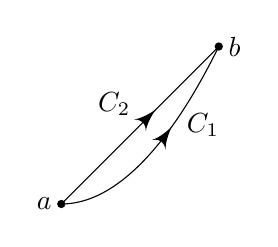
\begin{tikzpicture}
      \node [circ] {};
      \node [left] {$a$};
      \node at (2, 2) [circ] {};
      \node at (2, 2) [right] {$b$};
      \draw [->-=0.6] (0, 0) parabola (2, 2);
      \node at (1.8, 1) {$C_1$};
      \draw [->-=0.6] (0, 0) -- (2, 2) node [pos = 0.5, anchor = south east] {$C_2$};
    \end{tikzpicture}
  \end{center}
  We first integrate along the curve $C_1: \mathbf{r}(u) = (u, u^2, u^3)$. Then $\mathbf{r}'(u) = (1, 2u, 3u^2)$, and $\mathbf{F}(\mathbf{r}(u)) = (ue^{u^2}, u^6, u^3)$. So
  \begin{align*}
    \int_{C_1} \mathbf{F}\cdot \d\mathbf{r} &= \int_0^1 \mathbf{F}\cdot\mathbf{r}'(u)\; \d u\\
    &= \int_0^1 ue^{u^2} + 2u^7 + 3u^5\;\d u\\
    &= \frac{e}{2} -\frac{1}{2} + \frac{1}{4} + \frac{1}{2}\\
    &= \frac{e}{2} + \frac{1}{4}
  \end{align*}
  Now we try to integrate along another curve $C_2: \mathbf{r}(t) = (t, t, t)$. So $\mathbf{r}'(t) = (1,1, 1)$.
  \begin{align*}
    \int_{C_2} \mathbf{F}\cdot \d \mathbf{r} &= \int \mathbf{F}\cdot \mathbf{r}'(t)\d t\\
    &= \int_0^1 te^t + 2t^2\; \d t\\
    &= \frac{5}{3}.
  \end{align*}
  We see that the line integral depends on the curve $C$ in general, not just $\mathbf{a}, \mathbf{b}$.
\end{eg}

We can also use the arclength $s$ as parameter. Since $\d \mathbf{r} = \mathbf{t}\;\d s$, with $\mathbf{t}$ being the unit tangent vector, we have
\[
  \int_C \mathbf{F}\cdot \d \mathbf{r} = \int_C \mathbf{F}\cdot \mathbf{t}\;\d s.
\]
Note that we do not necessarily have to integrate $\mathbf{F}\cdot \mathbf{t}$ with respect to $s$. We can also integrate a scalar function as a function of $s$, $\int_C f(s)\;\d s$. By convention, this is calculated in the direction of increasing $s$. In particular, we have
\[
  \int_C 1\;\d s = \text{length of C}.
\]
\begin{defi}[Closed curve]
  A \emph{closed curve} is a curve with the same start and end point. The line integral along a closed curve is (sometimes) written as $\oint$ and is (sometimes) called the \emph{circulation} of $\mathbf{F}$ around $C$.
\end{defi}

Sometimes we are not that lucky and our curve is not smooth. For example, the graph of an absolute value function is not smooth. However, often we can break it apart into many smaller segments, each of which is smooth. Alternatively, we can write the curve as a sum of smooth curves. We call these \emph{piecewise smooth} curves.

\begin{defi}[Piecewise smooth curve]
  A \emph{piecewise smooth curve} is a curve $C = C_1 + C_2 + \cdots + C_n$ with all $C_i$ smooth with regular parametrisations. The line integral over a piecewise smooth $C$ is
  \[
    \int_C \mathbf{F}\cdot \d \mathbf{r} = \int_{C_1} \mathbf{F}\cdot \d \mathbf{r} + \int_{C_2} \mathbf{F}\cdot \d \mathbf{r} + \cdots + \int_{C_n} \mathbf{F}\cdot \d \mathbf{r}.
  \]
\end{defi}

\begin{eg}
  Take the example above, and let $C_3 = -C_2$. Then $C = C_1 + C_3$ is piecewise smooth but not smooth. Then
  \begin{align*}
    \oint _C \mathbf{F}\cdot \d \mathbf{r} &= \int_{C_1} \mathbf{F}\cdot \d \mathbf{r} + \int_{C_3} \mathbf{F}\cdot \d \mathbf{r}\\
    &= \left(\frac{e}{2} + \frac{1}{4}\right) - \frac{5}{3}\\
    &= -\frac{17}{12} + \frac{e}{2}.
  \end{align*}
  \begin{center}
    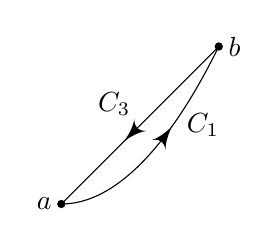
\begin{tikzpicture}
      \node [circ] {};
      \node [left] {$a$};
      \node at (2, 2) [circ] {};
      \node at (2, 2) [right] {$b$};
      \draw [->-=0.6] (0, 0) parabola (2, 2);
      \node at (1.8, 1) {$C_1$};
      \draw [->-=0.6] (2, 2) -- (0, 0) node [pos = 0.5, anchor = south east] {$C_3$};;
    \end{tikzpicture}
  \end{center}
\end{eg}
\subsection{Gradients and Differentials}
Recall that the line integral depends on the actual curve taken, and not just the end points. However, for some nice functions, the integral \emph{does} depend on the end points only.
\begin{thm}
  If $\mathbf{F} = \nabla f(\mathbf{r})$, then
  \[
    \int _C \mathbf{F}\cdot \mathbf{r} = f(\mathbf{b}) - f(\mathbf{a}),
  \]
  where $\mathbf{b}$ and $\mathbf{a}$ are the end points of the curve.

  In particular, the line integral does \emph{not} depend on the curve, but the end points only. This is the vector counterpart of the fundamental theorem of calculus. A special case is when $C$ is a closed curve, then $\oint_C \mathbf{F}\cdot \d \mathbf{r} = 0$.
\end{thm}

\begin{proof}
  Let $\mathbf{r}(u)$ be any parametrization of the curve, and suppose $\mathbf{a} = \mathbf{r}(\alpha)$, $\mathbf{b} = \mathbf{r}(\beta)$. Then
  \[
    \int_C \mathbf{F}\cdot \d \mathbf{r} = \int_C\nabla f\cdot \d \mathbf{r} = \int \nabla f\cdot \frac{\d \mathbf{r}}{\d u}\; \d u.
  \]
  So by the chain rule, this is equal to
  \[
    \int_\alpha^\beta \frac{\d }{\d u} (f(\mathbf{r}(u))) \;\d u = [f(\mathbf{r}(u))]_\alpha^\beta = f(\mathbf{b}) - f(\mathbf{a}).
  \]
\end{proof}

\begin{defi}[Conservative vector field]
  If $\mathbf{F} = \nabla f$ for some $f$, the $\mathbf{F}$ is called a \emph{conservative vector field}.
\end{defi}

The name \emph{conservative} comes from mechanics, where conservative vector fields represent conservative forces that conserve energy. This is since if the force is conservative, then the integral (ie. work done) about a closed curve is $0$, which means that we cannot gain energy after travelling around the loop.

It is convenient to treat differentials $\mathbf{F}\cdot \d \mathbf{r} = F_i \d x_i$ as if they were objects by themselves, which we can integrate along curves if we feel like doing so.

Then we can define
\begin{defi}[Exact differential]
  A differential $\mathbf{F}\cdot\d \mathbf{r}$ is \emph{exact} if there is an $f$ such that $\mathbf{F} = \nabla f$. Then
  \[
    \d f = \nabla f\cdot \d \mathbf{r} = \frac{\partial f}{\partial x_i} \d x_i.
  \]
\end{defi}

To test if this holds, we can use the necessary condition
\begin{prop}
  If $\mathbf{F} = \nabla f$ for some $f$, then
  \[
    \frac{\partial F_i}{\partial x_j} = \frac{\partial F_j}{\partial x_i}.
  \]
  This is because both are equal to $\partial^2 f/\partial x_i\partial x_j$.
\end{prop}

For an exact differential, the result from the previous section reads
\[
  \int_C \mathbf{F}\cdot \d \mathbf{r} = \int_C \d f = f(\mathbf{b}) - f(\mathbf{a}).
\]
Differentials can be manipulated using (for constant $\lambda, \mu$):
\begin{prop}
  \begin{align*}
    \d (\lambda f + \mu g) &= \lambda \d f + \mu \d g\\
    \d (fg) &= (\d f)g + f(\d g)
  \end{align*}
\end{prop}

Using these, it may be possible to find $f$ by inspection.

\begin{eg}
  Consider
  \[
    \int_C 3x^2 y\sin z\;\d x + x^3 \sin z \;\d y + x^3 y\cos z\;\d z.
  \]
  We see that if we integrate the first term with respect to $x$, we obtain $x^3 y\sin z$. We obtain the same thing if we integrate the second and third term. So this is equal to
  \[
    \int_C \d (x^3 y \sin z) = [x^3 y\sin z]^{\mathbf{b}}_{\mathbf{a}}.
  \]
\end{eg}

\subsection{Work and potential energy}
\begin{defi}[Work and potential energy]
  If $\mathbf{F}(\mathbf{r})$ is a force, then $\int_C \mathbf{F}\cdot \d \mathbf{r}$ is the \emph{work done} by the force along the curve $C$. It is the limit of a sum of terms $\mathbf{F}(\mathbf{r})\cdot \delta \mathbf{r}$, ie. the force along the direction of $\delta \mathbf{r}$.
\end{defi}

Consider a point particle moving under $\mathbf{F}(\mathbf{r})$ according to Newton's second law: $\mathbf{F}(\mathbf{r}) = m\ddot{\mathbf{r}}$.

Since the kinetic energy is defined as
\[
  T(t) = \frac{1}{2}m\dot{\mathbf{r}}^2,
\]
the rate of change of energy is
\[
  \frac{\d}{\d t}T(t) = m\dot{\mathbf{r}}\cdot \ddot{\mathbf{r}} = \mathbf{F}\cdot \mathbf{r}.
\]
Suppose the path of particle is a curve $C$ from $\mathbf{a} = \mathbf{r}(\alpha)$ to $\mathbf{b} = \mathbf{r}(\beta)$, Then
\[
  T(\beta) - T(\alpha) = \int_\alpha^\beta \frac{\d T}{\d t} \;\d t = \int_\alpha^\beta \mathbf{F}\cdot \dot{\mathbf{r}}\;\d t = \int_C \mathbf{F}\cdot \d \mathbf{r}.
\]
So the work done on the particle is the change in kinetic energy.

\begin{defi}[Potential energy]
  Given a conservative force $\mathbf{F} = -\nabla V$, $V(\mathbf{x})$ is the \emph{potential energy}. Then
  \[
    \int_C \mathbf{F}\cdot \d \mathbf{r} = V(\mathbf{a}) - V(\mathbf{b}).
  \]
\end{defi}
Therefore, for a conservative force, we have $\mathbf{F} = \nabla V$, where $V(\mathbf{r})$ is the potential energy.

So the work done (gain in kinetic energy) is the loss in potential energy. So the total energy $T + V$ is conserved, ie. constant during motion.

We see that energy is conserved for conservative forces. In fact, the converse is true --- the energy is conserved only for conservative forces.

\section{Integration in \texorpdfstring{$\R^2$ and $\R^3$}{R2 and R3}}
\subsection{Integrals over subsets of \texorpdfstring{$\R^2$}{R2}}
\begin{defi}[Surface integral]
  Let $D\subseteq \R^2$. Let $\mathbf{r} = (x, y)$ be in Cartesian coordinates. We can approximate $D$ by $N$ disjoint subsets of simple shapes, eg. triangles, parallelograms. These shapes are labelled by $I$ and have areas $\delta A_i$. \begin{center}
    \begin{tikzpicture}
      \draw [->] (0, 0) -- (6, 0) node [right] {$x$};
      \draw [->] (0, 0) -- (0, 4) node [above] {$y$};
      \draw (2, 1.6) -- (3.6, 1.6);
      \draw (2, 2) -- (3.6, 2);
      \draw (2, 2.4) -- (3.6, 2.4);
      \draw (2, 2.8) -- (3.6, 2.8);
      \draw (2.2, 1.4) -- (2.2, 3);
      \draw (2.6, 1.4) -- (2.6, 3);
      \draw (3, 1.4) -- (3, 3);
      \draw (3.4, 1.4) -- (3.4, 3);
      \draw plot [smooth cycle] coordinates {(1, 1) (2.5, 1.2) (4, 0.9) (4.2, 3.2) (1.5, 3)};
      \node at (4.2, 3.2) [anchor = south west] {$D$};
    \end{tikzpicture}
  \end{center}
  To integrate a function $f$ over $D$, we would like to take the sum $\sum f(\mathbf{r}_i) \delta A_i$, and take the limit as $\delta A_i \to 0$. But we need a condition stronger than simply $\delta A_i \to 0$. We won't want the areas to grow into arbitrarily long yet thin strips whose area decreases to 0. So we say that we find an $\ell$ such that each area can be contained in a disc of diameter $\ell$.

  Then we take the limit as $\ell \to 0$, $N\to \infty$, and the union of the pieces tends to $D$. For a function $f(\mathbf{r})$, we define the \emph{surface integral} as
  \[
    \int_D f(\mathbf{r}) \;\d A = \lim_{\ell\to 0}\sum _I f(\mathbf{r}_i)\delta A_i.
  \]
  where $\mathbf{r}_i$ is some point within each subset $A_i$. The integral \emph{exists} if the limit is well-defined (ie. the same regardless of what $A_i$ and $\mathbf{r}_i$ we choose before we take the limit) and exists.
\end{defi}
If we take $f = 1$, then the surface integral is the area of $D$.

On the other hand, if we put $z = f(x, y)$ and plot out the surface $z = f(x, y)$, then the area integral is the volume under the surface.

The definition allows us to take the $\delta A_i$ to be any weird shape we want. However, the sensible thing is clearly to take $A_i$ to be rectangles.

We choose the small sets in the definition to be rectangles, each of size $\delta A_I = \delta x\delta y$. We sum over subsets in a narrow horizontal strip of height $\delta y$ with $y$ and $\delta y$ held constant. Take the limit as $\delta x\to 0$. We get a contribution $\delta y\int_{x_y} f(y, x)\;\d x$ with range $x_y\in \{x: (x, y)\in D\}$.
\begin{center}
  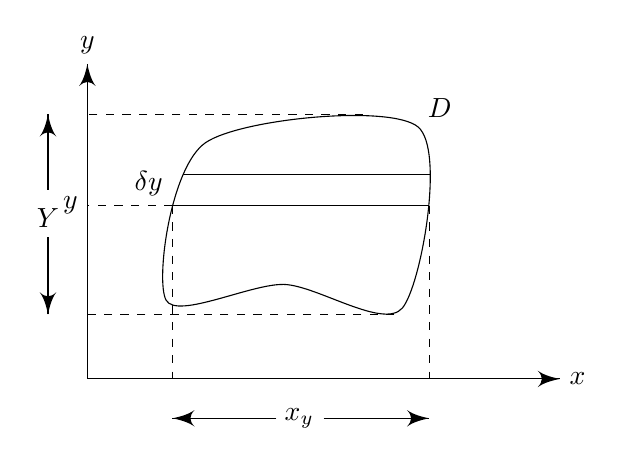
\begin{tikzpicture}
    \draw [->] (0, 0) -- (6, 0) node [right] {$x$};
    \draw [->] (0, 0) -- (0, 4) node [above] {$y$};
    \draw (1.08, 2.2) node [anchor = south east] {$\delta y$} -- (4.34, 2.2);
    \draw (1.22, 2.6) -- (4.36, 2.6);
    \draw [dashed] (1.08, 2.2) -- (1.08, 0);
    \draw [dashed] (4.34, 2.2) -- (4.34, 0);
    \draw [dashed] (1.08, 2.2) -- (0, 2.2) node [left] {$y$};
    \draw [->] (2.4, -0.5) -- (1.08, -0.5);
    \draw [->] (3, -0.5) node [left] {$x_y$} -- (4.34, -0.5);
    \draw plot [smooth cycle] coordinates {(1, 1) (2.5, 1.2) (4, 0.9) (4.2, 3.2) (1.5, 3)};
    \draw [dashed] (3.5, 3.36) -- (0, 3.36);
    \draw [dashed] (3.9, 0.82) -- (0, 0.82);
    \draw [->] (-0.5, 2.4) -- (-0.5, 3.36);
    \draw [->] (-0.5, 1.8) node [above] {$Y$} -- (-0.5, 0.82);
    \node at (4.2, 3.2) [anchor = south west] {$D$};
  \end{tikzpicture}
\end{center}
We sum over all such strips and take $\delta y\to 0$, giving

\begin{prop}
  \[
    \int_D f(x, y)\;\d A = \int_Y\left(\int_{x_y}f(x, y)\;\d x\right) \d y.
  \]
  with $x_y$ ranging over $\{x: (x, y) \in D\}$.
\end{prop}

Note that the range of the inner integral is given by a set $x_y$. This can be an interval, or many disconnected intervals, $x_y = [a_1, b_1]\cup [a_2, b_2]$. In this case,
\[
  \int_{x_y} f(x)\; \d x = \int_{a_1}^{b_1} f(x) \;\d x + \int_{a_2}^{b_2}f(x)\;\d x.
\]
This is useful if we want to integrate over a concave area and we have disconnected vertical strips.
\begin{center}
  \begin{tikzpicture}
    \draw [->] (0, 0) -- (6, 0) node [right] {$x$};
    \draw [->] (0, 0) -- (0, 4) node [above] {$y$};
    \draw plot [smooth cycle] coordinates {(1, 1) (4, 0.8) (4.2, 1.1) (3, 2) (4.1, 3) (1.2, 2.7)};
    \draw (3.2, 0.8) -- (3.2, 1.76);
    \draw (3.4, 0.8) -- (3.4, 1.61);
    \draw (3.2, 2.24) -- (3.2, 3.02);
    \draw (3.4, 2.4) -- (3.4, 3.04);
  \end{tikzpicture}
\end{center}
We could also do it the other way round, integrating over $y$ first, and come up with the result
\[
  \int_D f(x, y)\; \d A = \int_X\left(\int_{y_x}f(x, y)\; \d y\right) \d x.
\]
\begin{thm}[Fubini's theorem]
  If $f$ is a continuous function and $D$ is a compact (ie. closed and bounded) subset of $\R^2$, then
  \[
    \int\int f\;\d x\;\d y = \int\int f\;\d y\;\d x.
  \]
  While we have rather strict conditions for this theorem, it actually holds in many more cases, but those situations have to be checked manually.
\end{thm}
\begin{defi}[Area element]
  The \emph{area element} is $\d A$.
\end{defi}

\begin{prop}
  $\d A = \d x\;\d y$ in Cartesian coordinates.
\end{prop}

\begin{eg}
  We integrate over the triangle bounded by $(0, 0), (2, 0)$ and $(0, 1)$. We want to integrate the function $f(x, y) = x^2y$ over the area. So
  \begin{align*}
    \int _D f(x y)\;\d A &= \int_0^1 \left(\int_0^{2 - 2y}x^2y \;\d x\right)\; \d y\\
    &= \int_0^1 y\left[\frac{x^3}{3}\right]^{2 - 2y}_0 \;\d y\\
    &= \frac{8}{3}\int_0^1 y(1 - y)^3\;\d y\\
    &= \frac{2}{15}
  \end{align*}
  We can integrate it the other way round:
  \begin{align*}
    \int_D x^2 y\;\d A &= \int_0^2 \int_0^{1 - x/2}x^2y \;\d y\;\d x\\
    &= \int_0^2 x^2\left[\frac{1}{2}y^2\right]_0^{1 - x/2}\;\d x\\
    &= \int_0^2 \frac{x^2}{2} \left(1 - \frac{x}{2}\right)^2 \;\d x\\
    &= \frac{2}{15}
  \end{align*}
\end{eg}

Since it doesn't matter whether we integrate $x$ first or $y$ first, if we find it difficult to integrate one way, we can try doing it the other way and see if it is easier.

While this integral is tedious in general, there is a special case where it is substantially easier.
\begin{defi}[Separable function]
  A function $f(x, y)$ is separable if it can be written as $f(x, y) = h(y)g(x)$.
\end{defi}

\begin{prop}
  Take separable $f(x, y) = h(y)g(x)$ and $D$ be a rectangle $\{(x, y): a\leq x\leq b, c\leq y \leq d\}$. Then
  \[
    \int_Df(x, y)\;\d x\;\d y = \left(\int_a^b g(x)\;\d x\right)\left(\int_c^d h(y)\;\d y\right)
  \]
\end{prop}

\subsection{Change of variables for an integral in \texorpdfstring{$\R^2$}{R2}}
\begin{prop}
  Suppose we have a change of variables $(x, y)\leftrightarrow (u, v)$ that is smooth and invertible, with regions $D, D'$ in one-to-one correspondence. Then
  \[
    \int_D f(x, y)\;\d x\;\d y = \int_D f(x(u, v), y(u, v))|J|\;\d u\;\d v,
  \]
  where
  \[
    J = \frac{\partial (x, y)}{\partial (u, v)} =
    \begin{vmatrix}
      \dfrac{\partial x}{\partial u} & \dfrac{\partial x}{\partial v}\vspace{5pt}\\
      \dfrac{\partial y}{\partial u} & \dfrac{\partial y}{\partial v}\\
    \end{vmatrix}
  \]
  is the Jacobian. In other words,
  \[
    \;\d x\;\d y = |J|\;\d u\;\d v.
  \]
\end{prop}

\begin{proof}
  Since we are writing $(x(u, v), y(u, v))$, we are actually transforming from $(u, v)$ to $(x, y)$ and not the other way round.

  Suppose we start with an area $\delta A' = \delta u\delta v$ in the $(u, v)$ plane. Then by Taylors' theorem, we have
  \[
    \delta x = x(u + \delta u, v + \delta v) - x(u, v) \approx \frac{\partial x}{\partial u}\delta u + \frac{\partial x}{\partial v}\delta v.
  \]
  We have a similar expression for $\delta y$ and we obtain
  \[
    \begin{pmatrix}
      \delta x\\
      \delta y
    \end{pmatrix}
    \approx
    \begin{pmatrix}
      \frac{\partial x}{\partial u} & \frac{\partial x}{\partial v}\\
      \frac{\partial y}{\partial u} & \frac{\partial y}{\partial v}\\
    \end{pmatrix}
    \begin{pmatrix}
      \delta u\\
      \delta v
    \end{pmatrix}
  \]
  Recall from Vectors and Matrices that the determinant of the matrix is how much it scales up an area. So the area formed by $\delta x$ and $\delta y$ is $|J|$ times the area formed by $\delta u$ and $\delta v$. Hence
  \[
    \d x\;\d y = |J| \;\d u\;\d v.
  \]
\end{proof}

\begin{eg}
  We transform from $(x, y)$ to $(\rho, \varphi)$ with
  \begin{align*}
    x &= \rho\cos \varphi\\
    y &= \rho\sin \varphi
  \end{align*}
  We have previously calculated that $|J| = \rho$. So
  \[
    \d A = \rho \;\d \rho \;\d \varphi.
  \]
  Suppose we want to integrate a function over a quarter area $D$ of radius $R$.
  \begin{center}
    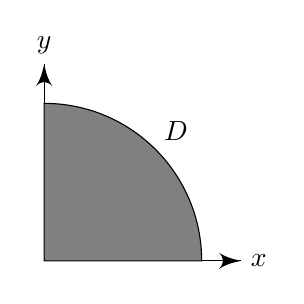
\begin{tikzpicture}
      \draw [->] (0, 0) -- (2.5, 0) node [right] {$x$};
      \draw [->] (0, 0) -- (0, 2.5) node [above] {$y$};
      \draw [fill=gray] (0, 0) -- (2, 0) arc (0:90:2) -- cycle;
      \node at (1.4, 1.4) [anchor=south west] {$D$};
    \end{tikzpicture}
  \end{center}
  Let the function to be integrated be $f = \exp(-(x^2 + y^2)/2) = \exp(-\rho^2/2)$. Then
  \begin{align*}
    \int f\;\d A &= \int f\rho\;\d\rho\;\d\varphi\\
    &=\int_{\rho=0}^R\left(\int_{\varphi=0}^{\pi/2}e^{-\rho^2/2}\rho \;\d \varphi\right)\delta \rho\\
    \intertext{Note that in polar coordinates, we are integrating over a rectangle and the function is separable. So this is equal to}
    &= \left[-e^{-\rho^2/2}\right]^R_0\left[\varphi\right]_0^{\pi/2}\\
    &= \frac{\pi}{2}\left( 1 - e^{-R^2/2}\right).\tag{$*$}
  \end{align*}
  Note that the integral exists as $R\to \infty$.

  Now we take the case of $x, y\to \infty$ and consider the original integral.
  \begin{align*}
    \int _D f\;\d A &= \int_{x = 0}^{\infty} \int_{y=0}^\infty e^{-(x^2 + y^2)/2}\;\d x\;\d y\\
    &= \left(\int_0^\infty e^{-x^2/2}\;\d x\right)\left(\int_0^\infty e^{-y^2/2}\;\d y\right)\\
    &= \frac{\pi}{2}
  \end{align*}
  where the last line is from (*). So each of the two integrals must be $\sqrt{\pi/2}$, ie.
  \[
    \int_0^\infty e^{-x^2/2}\;\d x = \sqrt{\frac{\pi}{2}}.
  \]

\end{eg}
\subsection{Generalization to \texorpdfstring{$\R^3$}{R3}}
We will do exactly the same thing as we just did, but with one more dimension:
\begin{defi}[Volume integral]
  Consider a volume $V\subseteq \R^3$ with position vector $\mathbf{r} = (x, y, z)$. We approximate $V$ by $N$ small disjoint subsets of some simple shape (eg. cuboids) labelled by $I$, volume $\delta V_I$, contained within a solid sphere of diameter $\ell$.

  Assume that as $\ell \to 0$ and $N\to \infty$, the union of the small subsets tend to $V$. Then
  \[
    \int_V f(\mathbf{r})\;\d V = \lim_{\ell \to 0} \sum_{I}f(\mathbf{r}_I^*) \delta V_I,
  \]
  where $\mathbf{r}_I^*$ is any chosen point in each small subset.
\end{defi}
To evaluate this, we can take $\delta V_I = \delta x \delta y \delta z$, and take $\delta x\to 0$, $\delta y\to 0$ and $\delta z$ in some order. For example,
\[
  \int_V f(\mathbf{r})\;\d v = \int_D \left(\int_{Z_{xy}}f(x, y, z)\;\d z\right)\;\d x\;\d y.
\]
So we integrate $f(x, y, z)$ over $z$ at each point $(x, y)$, then take the integral of that over the area containing all required $(x, y)$.

Alternatively, we can take the area integral first, and have
\[
  \int_V f(\mathbf{r})\;\d V = \int_z\left(\int_{D_Z} f(x, y, z)\;\d x\;\d y\right)\;\d z.
\]
Again, if we take $f = 1$, then we obtain the volume of $V$.

Often, $f(\mathbf{r})$ is the density of some quantity, and is usually denoted by $\rho$. For example, we might have mass density, charge density, or probability density. $\rho(\mathbf{r})\delta V$ is then the amount of quantity in a small volume $\delta V$ at $\mathbf{r}$. Then $\int_V \rho(\mathbf{r}) \;\d V$ is the total amount of quantity in $V$.

\begin{defi}[Volume element]
  The \emph{volume element} is $\d V$.
\end{defi}

\begin{prop}
  $\d V = \d x\; \d y\; \d z$.
\end{prop}

We can change variables by some smooth, invertible transformation $(x, y, z)\mapsto (u, v, w)$. Then
\begin{prop}
  \[
    \int_V f\;\d x\;\d y\;\d z = \int_V f|J|\;\d u\;\d v\;\d w,
  \]
  with
  \[
    J = \frac{\partial(x, y, z)}{\partial(u, v, w)} =
    \begin{vmatrix}
      \dfrac{\partial x}{\partial u} & \dfrac{\partial x}{\partial v} & \dfrac{\partial x}{\partial w}\vspace{5pt} \\
      \dfrac{\partial y}{\partial u} & \dfrac{\partial y}{\partial v} & \dfrac{\partial y}{\partial w}\vspace{5pt} \\
      \dfrac{\partial z}{\partial u} & \dfrac{\partial z}{\partial v} & \dfrac{\partial z}{\partial w}
    \end{vmatrix}
  \]
\end{prop}

\begin{prop}
  In cylindrical coordinates,
  \[
    \d V = \rho\;\d \rho\;\d \varphi\;\d z.
  \]
  In spherical coordinates
  \[
    \d V = r^2\sin\theta \;\d r\;\d \theta\;\d \varphi.
  \]
\end{prop}

\begin{proof}
  Loads of algebra.
\end{proof}

\begin{eg}
  Suppose $f(\mathbf{r})$ is spherically symmetric and $V$ is a sphere of radius $a$ centered on the origin. Then
  \begin{align*}
    \int_V f\;\d V &= \int_{r = 0}^a \int_{\theta = 0}^\pi \int_{\varphi = 0}^{2\pi} f(r)r^2 \sin\theta\;\d r\;\d \theta\;\d\varphi\\
    &= \int_0^a \d r\int_0^\pi \d \theta\int_0^{2\pi} \d \varphi \;r^2 f(r) \sin \theta\\
    &= \int_0^a \; r^2 f(r) \d r\Big[-\cos \theta\Big]_0^\pi \Big[\varphi\Big]_0^{2\pi}\\
    &= 4\pi\int_0^a f(r)r^2 \;\d r.
  \end{align*}
  where we separated the integral into three parts as in the area integrals.

  Note that in the second line, we rewrote the integrals to write the differentials next to the integral sign. This is simply a different notation that saves us from writing $r = 0$ etc. in the limits of the integrals.

  This is a useful general result. We understand it as the sum of spherical shells of thickness $\delta r$ and volume $4\pi r^2 \delta r$.

  If we take $f = 1$, then we have the familiar result that the volume of a sphere is $\frac{4}{3}\pi a^3$.
\end{eg}

\begin{eg}
  Consider a volume within a sphere of radius $a$ with a cylinder of radius $b$ ($b < a$) removed. The region is defined as
  \begin{align*}
    x^2 + y^2 + z^2 &\leq a^2\\
    x^2 + y^2 &\geq b^2.
  \end{align*}
  \begin{center}
    \begin{tikzpicture}
      \begin{scope}
        \clip (-.99, 2) rectangle (-3, -2.1) (.99, 2) rectangle (3, -2.1);
        \draw circle [radius=2];
      \end{scope}
      \draw (0, 1.72) circle [x radius=1, y radius = 0.15];
      \draw [dash pattern= on 4pt off 4pt] (1, -1.72) arc (0: 180:1 and 0.15);
      \draw (-1, -1.72) arc (180: 360:1 and 0.15);
      \draw [dash pattern= on 4pt off 4pt] (1, 1.72) -- (1, -1.72);
      \draw [dash pattern= on 4pt off 4pt] (-1, 1.72) -- (-1, -1.72);
      \draw [dash pattern= on 2pt off 2pt] (0, 0) -- (1, 1.72) node [pos = 0.5, anchor = north west] {$a$};
      \draw [dash pattern= on 2pt off 2pt] (0, 0) -- (-1, 0) node [pos = 0.5, above] {$b$};
    \end{tikzpicture}
  \end{center}
  We use cylindrical coordinates. The second criteria gives
  \[
    b \leq \rho \leq a.
  \]
  For the $x^2 + y^2 + z^2 \leq a^2$ criterion, we have
  \[
    -\sqrt{a^2 - \rho^2} \leq z \leq \sqrt{a^2 - \rho^2}.
  \]
  So the volume is
  \begin{align*}
    \int_V \;\d V &= \int_b^a\d \rho\int_0^{2\pi}\d \varphi \int_{-\sqrt{a^2 - \rho^2}}^{\sqrt{a^2 - \rho^2}}\d z\; \rho\\
    &= 2\pi\int_b^a 2\rho\sqrt{a^2 - \rho^2}\;\d \rho\\
    &= 2\pi \left[\frac{2}{3}(a^2 - \rho^2)^{3/2}\right]^a_b\\
    &= \frac{4}{3}\pi (a^2 - b^2)^{3/2}.
  \end{align*}
\end{eg}
\begin{eg}
  Suppose the density of electric charge $\rho(\mathbf{r}) = \rho_0 \frac{z}{a}$ in a hemisphere $H$ of radius $a$, with $z \geq 0$. What is the total charge of $H$?

  We use spherical polars. So
  \[
    V \leq a,\quad 0 \leq \varphi \leq 2\pi,\quad 0 \leq \theta \leq \frac{\pi}{2}.
  \]
  We have
  \[
    \rho(\mathbf{r}) = \frac{\rho_0}{a}r\cos \theta.
  \]
  The total charge $Q$ in $H$ is
  \begin{align*}
    \int_H \rho \;\d V &= \int_0^a\d r\int_0^{\pi/2}\d \theta\int_0^{2\pi}\d\varphi\; \frac{\rho_0}{a}r\cos\theta r^2\sin\theta\\
    &= \frac{\rho_0}{a}\int_0^a r^3 \;\d r \int_0^{\pi/2}\sin\theta \cos\theta\;\d \theta \int_0^{2\pi}\;\d \varphi\\
    &= \frac{\rho_0}{a}\left[\frac{r^4}{4}\right]^a_0\left[\frac{1}{2}\sin^2\theta\right]^{\pi/2}_0 [\varphi]^{2\pi}_0\\
    &= \frac{\rho_0 \pi a^3}{4}.
  \end{align*}
\end{eg}
\subsection{Further generalizations}
\subsubsection*{Integration in \texorpdfstring{$R^n$}{Rn}}
$\int_D f(x_1, x_2, \cdots x_n)\;\d x_1 \;\d x_2\cdots\;\d x_n$ is simply the integration over an $n$-dimensional volume. The change of variable formula is
\begin{prop}
  \[
    \int_D f(x_1, x_2, \cdots x_n)\;\d x_1 \;\d x_2\cdots\;\d x_n = \int_{D'} f(\{x_i(\mathbf{u})\}) |J| \;\d u_1\;\d u_2\cdots\;\d u_n.
  \]
\end{prop}

\subsubsection*{Change of variables for \texorpdfstring{$n = 1$}{n = 1}}
In the $n = 1$ case, the Jacobian is $\frac{\d x}{\d u}$. However, we use the following formula for change of variables:
\[
  \int_D f(x) \;\d x = \int_{D'} f(x(u))\left|\frac{\d x}{\d u}\right| \;\d u.
\]
We introduce the modulus because of our natural convention about integrating over $D$ and $D'$. If $D = [a, b]$ with $a < b$, we write $\int_a^b$. But if $a\mapsto \alpha$ and $b \mapsto \beta$, but $\alpha > \beta$, we would like to write $\int_\beta ^\alpha$ instead, so we introduce the modulus in the 1D case.

To show that the modulus is the right thing to do, we check case by case: If $a < b$ and $\alpha < \beta$, then $\frac{\d x}{\d u}$ is positive, and we have, as expected
\[
  \int_a^b f(x)\;\d x = \int_\alpha^\beta f(u)\frac{\d x}{\d u}\;\d u.
\]
If $\alpha > \beta$, then $\frac{\d x}{\d u}$ is negative. So
\[
  \int_a^b f(x)\;\d x = \int_\alpha^\beta f(u)\frac{\d x}{\d u}\;\d u = -\int_\beta^\alpha f(u)\frac{\d x}{\d u}\;\d u.
\]
By taking the absolute value of $\frac{\d x}{\d u}$, we ensure that we always have the numerically smaller bound as the lower bound.

This is not easily generalized to higher dimensions, so we don't employ the same trick in other cases.

\subsubsection*{Vector-valued integrals}
We can define $\int_V \mathbf{F}(\mathbf{r})\;\d V$ in a similar way to $\int_V f(\mathbf{r})\;\d V$as the limit of a sum over small contributions of volume. In practice, we integrate them componentwise. If
\[
  \mathbf{F}(\mathbf{r}) = F_{i}(\mathbf{r})\mathbf{e}_i,
\]
then
\[
  \int_V \mathbf{F}(\mathbf{r})\;\d V = \int_V (F_i(\mathbf{r})\;\d V)\mathbf{e}_i.
\]
For example, if a mass has density $\rho (\mathbf{r})$, then its mass is
\[
  M = \int_V \rho(\mathbf{r})\;\d V
\]
and its center of mass is
\[
  \mathbf{R} = \frac{1}{M}\int_V \mathbf{r}\rho (\mathbf{r})\;\d V.
\]
\begin{eg}
  Consider a solid hemisphere $H$ with $r \leq a$, $z \geq 0$ with uniform density $\rho$. The mass is
  \[
    M = \int_H \rho \;\d V = \frac{2}{3}\pi a^3\rho.
  \]
  Now suppose that $\mathbf{R} = (X, Y, Z)$. By symmetry, we expect $X = Y = 0$. We can find this formally by
  \begin{align*}
    X &= \frac{1}{M}\int_H x\rho \;\d V\\
    &= \frac{\rho}{M}\int_0^a \int_0^{\pi/2}\int_0^{2\pi}xr^2 \sin \theta\;\d \varphi\;\d \theta\;\d r\\
    &= \frac{\rho}{M}\int_0^{a}r^3\;\d r\times \int_0^{\pi/2}\sin^2\theta\;\d \theta\times \int_0^{2\pi}\cos\varphi\;\d \varphi\\
    &= 0
  \end{align*}
  as expected. Note that it evaluates to 0 because the integral of $\cos$ from $0$ to $2\pi$ is 0. Similarly, we obtain $Y = 0$.

  Finally, we find $Z$.
  \begin{align*}
    Z &= \frac{\rho}{M}\int_0^a r^3\;\d r \int_0^{\pi/2}\sin\theta\cos\theta\;\d \theta \int_0^{2\pi}\;\d \varphi\\
    &= \frac{r}{M}\left[\frac{a^4}{4}\right]\left[\frac{1}{2}\sin^2\theta\right]_0^{\pi/2}2\pi\\
    &= \frac{3a}{8}.
  \end{align*}
  So $\mathbf{R} = (0, 0, 3a/8)$.
\end{eg}

\section{Surfaces and surface integrals}
\subsection{Surfaces and Normal}
Let $f$ be a smooth function on $\R^3$ and a constant $c$. Then $f(\mathbf{r}) = c$ defines a smooth surface (eg. $x^2 + y^2 + z^2 = 1$ denotes the unit sphere). Consider any curve $\mathbf{r}(u)$ on $S$. Then by the chain rule, if we differentiate $f(\mathbf{r}) = c$ with respect to $u$, we obtain
\[
  \frac{\d }{\d u}[f(\mathbf{r}(u))] = \nabla f\cdot \frac{\d \mathbf{r}}{\d u} = 0.
\]
This means that $\nabla f$ is always perpendicular to $\frac{\d \mathbf{r}}{\d u}$. Since $\frac{\d \mathbf{r}}{\d u}$ is the tangent to the curve, $\nabla f$ is perpendicular to the tangent. Since this is true for \emph{any} curve $\mathbf{r}(u)$, $\nabla f$ is perpendicular to any tangent of the surface. Therefore
\begin{prop}
  $\nabla f$ is the normal to the surface $f(\mathbf{r}) = c$.
\end{prop}

\begin{eg}\leavevmode
  \begin{enumerate}
    \item Take the sphere $f(\mathbf{r}) = x^2 + y^2 + z^2 = c$ for $c > 0$. Then $\nabla f = 2(x, y, z) = 2\mathbf{r}$, which is clearly normal to the sphere.
    \item Take $f(\mathbf{r}) = x^2 + y^2 - z^2 = c$, which is a hyperboloid. Then $\nabla f = 2(x, y, -z)$.

      In the special case where $c = 0$, we have a double cone, with a singular apex $\mathbf{0}$. Here $\nabla f = \mathbf{0}$, and we cannot find a meaningful direction of normal.
  \end{enumerate}
\end{eg}

\begin{defi}[Boundary]
  A surface $S$ can be defined to have a \emph{boundary} $\partial S$ consisting of a piecewise smooth curve. If we define $S$ as in the above examples but with the additional restriction $z \geq 0$, then $\partial S$ is the circle $x^2 + y^2 = c$, $z = 0$.

  A surface is \emph{bounded} if it can be contained in a solid sphere, \emph{unbounded} otherwise. A bounded surface with no boundary is called \emph{closed} (eg. sphere).
\end{defi}
\begin{eg}\leavevmode
  \begin{center}
    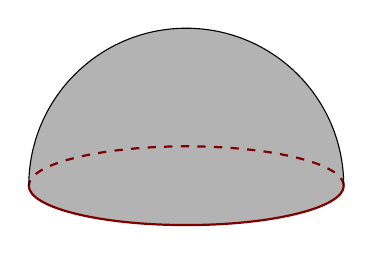
\begin{tikzpicture}
      \draw [draw=none, fill=gray, opacity=0.6] (-2, 0) arc (180:360:2 and 0.5) arc (0:180:2);
      \draw [mred, thick, dashed] (2, 0) arc (0:180:2 and 0.5);
      \draw [mred, thick] (-2, 0) arc (180:360:2 and 0.5);
      \draw (2, 0) arc (0:180:2);
    \end{tikzpicture}
  \end{center}
  The boundary of a hemisphere is a circle (drawn in red).
\end{eg}

\begin{defi}[Orientable surface]
  At each point, there is a unit normal $\mathbf{n}$ that's unique up to a sign.

  If we can find a consistent choice of $\mathbf{n}$ that varies smoothly across $S$, then we say $S$ is \emph{orientable}, and the choice of sign of $\mathbf{n}$ is called the \emph{orientation} of the surface.
\end{defi}
Most surfaces we encounter are orientable. For example, for a sphere, we can declare that the normal should always point outwards. A notable example of a non-orientable surface is the M\"obius strip (or Klein bottle).

For simple cases, we can describe the orientation as ``inward'' and ``outward''.

\subsection{Parametrized surfaces and area}
A surface $S$ can also be parametrised by $\mathbf{r}(u, v)$ with parameters $u, v$. $S$ is swept out as $u$ and $v$ vary in some region $D$. By the chain rule,
\[
  \delta \mathbf{r} = \frac{\partial \mathbf{r}}{\partial u}\delta u + \frac{\partial \mathbf{r}}{\partial v}\delta v + o(\delta u, \delta v).
\]
$\frac{\partial \mathbf{r}}{\delta u}$ and $\frac{\partial \mathbf{r}}{\partial v}$ are tangent vectors to curves on $S$ with $v$ and $u$ constant respectively.

\begin{defi}[Regular parametrization]
  A parametrization is \emph{regular} if for all $u, v$,
  \[
    \frac{\partial \mathbf{r}}{\partial u}\times \frac{\partial \mathbf{r}}{\partial v} \not = 0,
  \]
  ie. there are always two independent tangent directions.
\end{defi}
The parametrizations we use will all be regular.

The small changes $\delta u, \delta v$ make a small parallelogram on $S$. Up to $o$-terms, it has a vector area of
\[
  \delta \mathbf{S} = \frac{\partial \mathbf{r}}{\delta u}\times \frac{\partial \mathbf{r}}{\partial v} = \mathbf{n}\;\delta S.
\]
The order of $u, v$ gives the choice of the sign of the unit normal. By summing and taking limits, the area of $S$ is
\[
  \int_S \d S = \int_D \left|\frac{\partial \mathbf{r}}{\partial u}\times \frac{\partial \mathbf{r}}{\partial v}\right| \d u\;\d v
\]
\begin{prop}
  \[
    \d S = \left|\frac{\partial \mathbf{r}}{\partial u}\times \frac{\partial \mathbf{r}}{\partial v}\right|\;\d u\;\d v
  \]
  is the \emph{scalar area element}.
\end{prop}

\begin{eg}
  Let $S$ be part of a sphere of radius $a$ with $0 \leq \theta \leq \alpha$.
  \begin{center}
    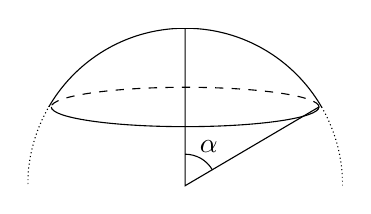
\begin{tikzpicture}
      \begin{scope}
        \clip (-2, 1) rectangle (2, 0);
        \draw [densely dotted] circle [radius=2];
      \end{scope}
      \begin{scope}
        \clip (-2, 2) rectangle (2, 1);
        \draw circle [radius=2];
      \end{scope}
      \draw [dashed] (1.7, 1) arc (0:180:1.7 and 0.25);
      \draw (-1.7, 1) arc (180:360:1.7 and 0.25);
      \draw (1.7, 1) -- (0, 0) -- (0, 2);
      \draw (0, 0.4) arc (90:30:.4);
      \node at (0.3, 0.5) {$\alpha$};
    \end{tikzpicture}
  \end{center}
  then
  \[
    \mathbf{r}(\theta, \varphi) = (a\cos\varphi\sin \theta, a\sin \theta\sin \varphi, a\cos \theta) = a\mathbf{e}_r.
  \]
  Then
  \[
    \frac{\partial \mathbf{r}}{\partial \theta} = a\mathbf{e}_\theta.
  \]
  Similarly, we have
  \[
    \frac{\partial \mathbf{r}}{\partial \varphi} = a\sin \theta \mathbf{e}_\varphi.
  \]
  Then
  \[
    \frac{\partial \mathbf{r}}{\partial \theta}\times \frac{\partial \mathbf{r}}{\partial \varphi} = a^2\sin \theta\, \mathbf{e}_r.
  \]
  So
  \[
    \d S = a^2\sin \theta\;\d \theta\;\d \varphi.
  \]
  Our bounds are $0 \leq \theta \leq \alpha$, $0 \leq \varphi \leq 2\pi$.

  Then the area is
  \[
    \int_0^{2\pi}\int_0^{\alpha} a^2\sin \theta\;\d \theta \;\d \varphi = 2\pi a^2(1 - \cos\alpha).
  \]
\end{eg}
\subsection{Surface integral of vector fields}
Let $S$ be a smooth surface parametrized by $\mathbf{r}(u, v)$, where $(u, v)$ takes values in $D$.
\begin{defi}[Surface integral]
  The \emph{surface integral} or $\emph{flux}$ of a vector field $\mathbf{F}(\mathbf{r})$ over $S$ is defined by
  \[
    \int_S \mathbf{F}(\mathbf{r})\cdot \d \mathbf{S} = \int_S \mathbf{F}(\mathbf{r})\cdot \mathbf{n}\;\d S = \int_D \mathbf{F}(\mathbf{r}(u, v))\cdot \left(\frac{\partial \mathbf{r}}{\partial u}\times \frac{\partial \mathbf{r}}{\partial v}\right)\;\d u\;\d v.
  \]
  Intuitively, this is the total amount of $\mathbf{F}$ passing through $S$. For example, if $\mathbf{F}$ is the electric field, the flux is the amount of electric field passing through a surface.
\end{defi}

For a given orientation, the integral $\int \mathbf{F}\cdot \d \mathbf{S}$ is independent of the parametrization. Changing orientation is equivalent to changing the sign of $\mathbf{n}$, which is in turn equivalent to changing the order of $u$ and $v$ in the definition of $S$, which is also equivalent to changing the sign of the flux integral.

\begin{eg}
  Consider a sphere of radius $a$, $\mathbf{r}(\theta, \varphi)$. Then
  \[
    \frac{\partial \mathbf{r}}{\partial \theta} = a\mathbf{e}_\theta,\quad \frac{\partial \mathbf{r}}{\partial \varphi} = a\sin \theta \mathbf{e}_\varphi.
  \]
  The vector area element is
  \[
    \d \mathbf{S} = a^2\sin \theta \mathbf{e}_r \;\d \theta\; \d\varphi,
  \]
  taking the outward normal $\mathbf{n} = \mathbf{e}_r = \mathbf{r}/a$.

  Suppose we want to calculate the fluid flux through the surface. The \emph{velocity field} $\mathbf{u}(\mathbf{r})$ of a fluid gives the motion of a small volume of fluid $\mathbf{r}$. Assume that $\mathbf{u}$ depends smoothly on $\mathbf{r}$ (and $t$). For any small area $\delta S$, on a surface $S$, the volume of fluid crossing it in time $\delta t$ is $\mathbf{u}\cdot \delta \mathbf{S}\; \delta t$.
  \begin{center}
    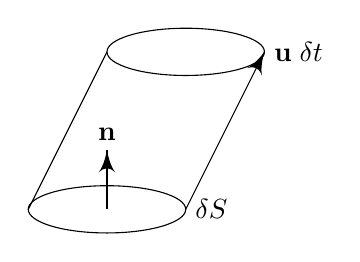
\begin{tikzpicture}
      \draw circle [x radius = 1, y radius = 0.3];
      \node at (1, 0) [right] {$\delta S$};
      \draw (1, 2) circle [x radius = 1, y radius = 0.3];
      \draw (-1, 0) -- (0, 2);
      \draw [->] (1, 0) -- (2, 2) node [right] {$\mathbf{u}\;\delta t$};
      \draw [->] (0, 0) -- (0, .75) node [above] {$\mathbf{n}$};
    \end{tikzpicture}
  \end{center}
  So the flux of $\mathbf{u}$ over at time $\delta t$ is
  \[
    \delta t\int_S \mathbf{u}\cdot \d \mathbf{S}.
  \]
  So $\int_S \mathbf{u}\cdot \d \mathbf{S}$ is the \emph{rate} of volume crossing $S$.

  For example, let $\mathbf{u} = (-x, 0, z)$ and $S$ be the section of a sphere of radius $a$ with $0 \leq \varphi \leq$ and $0 \leq \theta \leq \alpha$. Then
  \[
    \d \mathbf{S} = a^2 \sin \theta \mathbf{n}\;\d \varphi \;\d \theta,
  \]
  with
  \[
    \mathbf{n} = \frac{\mathbf{r}}{a} = \frac{1}{a}(x, y, z).
  \]
  So
  \[
    \mathbf{n}\cdot \mathbf{u} = \frac{1}{a}(-x^2 + z^2) = a(-\sin^2\theta\cos^2\varphi + \cos^2 \theta).
  \]
  Therefore
  \begin{align*}
    \int_S \mathbf{u}\cdot \d \mathbf{S} &= \int_0^\alpha \int_0^{2\pi} a^3 \sin \theta[(\cos^2\theta - 1) \cos^2 \varphi + \cos^2 \theta]\;\d \varphi\;\d \theta\\
    &= \int_0^\alpha a^3\sin \theta[\pi(cos^2\theta - 1) + 2\pi \cos^2\theta]\; \d \theta\\
    &=\int_0^\alpha a^3\pi(3\cos^3 \theta - 1)\sin \theta\;\d \theta\\
    &= \pi a^3[cos\theta - \cos^3 \theta]_0^\alpha\\
    &= \pi a^3 \cos \alpha\sin^2 \alpha.
  \end{align*}
\end{eg}

What happens when we change parametrization? Let $\mathbf{r}(u, v)$ and $\mathbf{r}(\tilde{u}, \tilde{v})$ be two regular parametrizations for the surface. By the chain rule,
\begin{align*}
  \frac{\partial \mathbf{r}}{\partial u} &= \frac{\partial \mathbf{r}}{\partial \tilde{u}}\frac{\partial\tilde{u}}{\partial u} + \frac{\partial \mathbf{r}}{\partial \tilde{v}}\frac{\partial\tilde{v}}{\partial u}\\
  \frac{\partial \mathbf{r}}{\partial v} &= \frac{\partial \mathbf{r}}{\partial \tilde{u}}\frac{\partial\tilde{u}}{\partial v} + \frac{\partial \mathbf{r}}{\partial \tilde{v}}\frac{\partial\tilde{v}}{\partial v}
\end{align*}
So
\[
  \frac{\partial \mathbf{r}}{\partial u}\times\frac{\partial\mathbf{r}}{\partial v} = \frac{\partial (\tilde{u}, \tilde{v})}{\partial (u, v)} \frac{\partial \mathbf{r}}{\partial \tilde {u}}\times\frac{\partial\mathbf{r}}{\partial \tilde{v}}
\]
where $\frac{\partial (\tilde{u}, \tilde{v})}{\partial(u, v)}$ is the Jacobian.

Since
\[
  \d \tilde{u}\;\d \tilde{v} = \frac{\partial (\tilde{u}, \tilde{v})}{\partial (u, v)}\;\d u\;\d v,
\]
We recover the formula
\[
  \d S = \left|\frac{\partial \mathbf{r}}{\partial u}\times\frac{\partial\mathbf{r}}{\partial v}\right|\;\d u\;\d v = \left|\frac{\partial \mathbf{r}}{\partial \tilde {u}}\times\frac{\partial\mathbf{r}}{\partial \tilde{v}}\right| \;\d \tilde{u}\;\d \tilde{v}.
\]
Similarly, we have
\[
  \d \mathbf{S} = \frac{\partial \mathbf{r}}{\partial u}\times\frac{\partial\mathbf{r}}{\partial v}\;\d u\;\d v = \frac{\partial \mathbf{r}}{\partial \tilde {u}}\times\frac{\partial\mathbf{r}}{\partial \tilde{v}} \;\d \tilde{u}\;\d \tilde{v}.
\]
provided $(u, v)$ and $(\tilde{u}, \tilde{v})$ have the same orientation.
\subsection{Change of variables in \texorpdfstring{$\R^2$ and $\R^3$}{R2 and R3} revisited}
In this section, we derive our change of variable formulae in a slightly different way.

\subsubsection*{Change of variable formula in \texorpdfstring{$\R^2$}{R2}}
We first derive the 2D change of variable formula from the 3D surface integral formula.

Consider a subset $S$ of the plane $\R^2$ parametrized by $\mathbf{r}(x(u, v), y(u, v))$. We can embed it to $\R^3$ as $\mathbf{r}(x(u, v), y(u, v), 0)$. Then
\[
  \frac{\partial \mathbf{r}}{\partial u}\times \frac{\partial\mathbf{r}}{\partial v} = (0, 0, J),
\]
with $J$ being the Jacobian.
Therefore
\[
  \int_S f(\mathbf{r})\;\d S = \int_D f(\mathbf{r}(u, v)) \left|\frac{\partial \mathbf{r}}{\partial u}\times \frac{\partial \mathbf{r}}{\partial v}\right| \;\d u\;\d v= \int_D f(\mathbf{r}(u, v))|J|\;\d u\;\d v,
\]
and we recover the formula for changing variables in $\R^2$.

\subsubsection*{Change of variable formula in \texorpdfstring{$R^3$}{R3}}
In $\R^3$, suppose we have a volume parametrised by $\mathbf{r}(u, v, w)$. Then
\[
  \delta \mathbf{r} = \frac{\partial \mathbf{r}}{\partial u}\delta u + \frac{\partial \mathbf{r}}{\partial v}\delta v + \frac{\partial \mathbf{r}}{\partial w}\delta w + o(\delta u, \delta v, \delta w).
\]
Then the cuboid $\delta u, \delta v, \delta w$ in $u, v, w$ space is mapped to a parallelopiped of volume
\[
  \delta V = \left|\frac{\partial \mathbf{r}}{\partial u}\delta u\cdot \left( \frac{\partial \mathbf{r}}{\partial v}\delta v \times \frac{\partial \mathbf{r}}{\partial w}\delta w\right)\right| = |J|\;\delta u\; \delta v\;\delta w.
\]
So $\d V = |J|\; \d u\; \d v\; \d w$.

\section{Geometry of curves and surfaces}
Let $\mathbf{r}(s)$ be a curve parametrized by arclength $s$. Since $\mathbf{t}(s) = \frac{\d \mathbf{r}}{\d s}$ is a unit vector, $\mathbf{t}\cdot \mathbf{t} = 1$. Differentiating yields $\mathbf{t}\cdot \mathbf{t}' = 0$. So $\mathbf{t}'$ is a normal to the curve if $\mathbf{t}' \not= 0$.

We define the following:
\begin{defi}[Principal normal and curvature]
  Write $\mathbf{t}' = \kappa \mathbf{n}$, where $\mathbf{n}$ is a unit vector and $\kappa > 0$. Then $\mathbf{n}(s)$ is called the \emph{principal normal} and $\kappa(s)$ is called the \emph{curvature}.
\end{defi}
Note that we \emph{must} be differentiating against $s$, not any other parametrization! If the curve is given in another parametrization, we can either change the parametrization or use the chain rule.

We take a curve that can Taylor expanded around $s = 0$. Then
\[
  \mathbf{r}(s) = \mathbf{r}(0) + s\mathbf{r}'(0) + \frac{1}{2}s^2 \mathbf{r}''(0) + O(s^3).
\]
We know that $\mathbf{r}' = \mathbf{t}$ and $\mathbf{r}'' = \mathbf{t}'$. So we have
\[
  \mathbf{r}(s) = \mathbf{r}(0) + s\mathbf{t}(0) + \frac{1}{2}\kappa(0) s^2 \mathbf{n} + O(s^3).
\]
How can we interpret $\kappa$ as the curvature? Suppose we want to approximate the curve near $\mathbf{r}(0)$ by a circle. We would expect a more ``curved'' curve would be approximated by a circle of smaller radius. So $\kappa$ should be inversely proportional to the radius of the circle. In fact, we will show that $\kappa = 1/a$, where $a$ is the radius of the best-fit circle.

Consider the vector equation for a circle passing through $\mathbf{r}(0)$ with radius $a$ in the plane defined by $\mathbf{t}$ and $\mathbf{n}$.
\begin{center}
  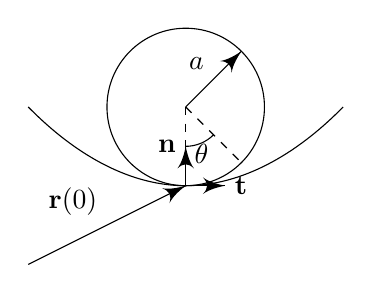
\begin{tikzpicture}
    \draw circle [radius = 1];
    \draw [->] (0, 0) -- (0.707, 0.707) node [anchor = south east, pos = 0.5] {$a$};
    \draw [->] (-2, -2) -- (0, -1) node [anchor = south east, pos = 0.5] {$\mathbf{r}(0)$};
    \draw [->] (0, -1) -- (0.5, -1) node [right] {$\mathbf{t}$};
    \draw [->] (0, -1) -- (0, -0.5) node [left] {$\mathbf{n}$};
    \draw [dashed] (0, 0) -- (0, -1);
    \draw [dashed] (0, 0) -- (0.707, -0.707);
    \draw (0, -0.5) arc (270:315:0.5);
    \node at (0.2, -0.6) {$\theta$};
    \draw (-2, 0) parabola bend (0, -1) (2, 0);
  \end{tikzpicture}
\end{center}
Then the equation of the circle is
\[
  \mathbf{r} = \mathbf{r}(0) + a(1 - \cos \theta) \mathbf{n} + a\sin \theta \mathbf{t}.
\]
We can expand this to obtain
\[
  \mathbf{r} = \mathbf{r}(0) + a\theta \mathbf{t} + \frac{1}{2}\theta^2 a\mathbf{n} + o(\theta^3).
\]
Since the arclength $s = a\theta$, we obtain
\[
  \mathbf{r} = \mathbf{r}(0) + s\mathbf{t} + \frac{1}{2}\frac{1}{a}s^2\mathbf{n} + O(s^3).
\]
As promised, $\kappa = 1/a$, for $a$ the radius of the circle of best fit.

\begin{defi}[Radius of curvature]
  The \emph{radius of curvature} of a curve at a point $\mathbf{r}(s)$ is $1/\kappa(s)$.
\end{defi}
Since we are in 3D, given $\mathbf{t}(s)$ and $\mathbf{n}(s)$, there is another normal to the curve. We can add a third normal to generate an orthonormal basis.
\begin{defi}[Binormal]
  The \emph{binormal} of a curve is $\mathbf{b} = \mathbf{t}\times \mathbf{n}$.
\end{defi}

We can define the torsion similar to the curvature, but with the binormal instead of the tangent.\footnote{This was not taught in lectures, but there is a question on the example sheet about the torsion, so I might as well include it here.}

\begin{defi}[Torsion] Let $\mathbf{b}' = -\tau \mathbf{n}$. Then $\tau$ is the \emph{torsion}.
\end{defi}
Note that this makes sense, since $\mathbf{b}'$ is both perpendicular to $\mathbf{t}$ and $\mathbf{b}$, and hence must be in the same direction as $\mathbf{n}$. ($\mathbf{b}' = \mathbf{t}'\times \mathbf{n} + \mathbf{t}\times \mathbf{n}' = \mathbf{t}\times \mathbf{n}'$, so $\mathbf{b}'$ is perpendicular to $\mathbf{t}$; and $\mathbf{b} \cdot \mathbf{b} = 1\Rightarrow \mathbf{b}\cdot \mathbf{b}' = 0$. So $\mathbf{b}'$ is perpendicular to $\mathbf{b}$).

The geometry of the curve is encoded in how this basis ($\mathbf{t}, \mathbf{n}, \mathbf{b}$) changes along it. This can be specified by two scalar functions of arc length --- the curvature $\kappa(s)$ and the \emph{torsion} $\tau(s)$ (which determines what the curve looks like to third order in its Taylor expansions and how the curve lifts out of the $\mathbf{t}, \mathbf{r}$ plane).

\subsubsection*{Surfaces and intrinsic geometry*}
We can study the geometry of surfaces through curves which lie on them. At a given point $P$ at a surface $S$ with normal $\mathbf{n}$, consider a plane containing $\mathbf{n}$. The intersection of the plane with the surface yields a curve on the surface through $P$. This curve has a curvature $\kappa$ at $P$.

If we choose different planes containing $\mathbf{n}$, we end up with different curves of different curvature. Then we define the following:
\begin{defi}[Principal curvature]
  The \emph{principal curvatures} of a surface at $P$ are the minimum and maximum possible curvature of a curve through $P$, denoted $\kappa_{\min}$ and $\kappa_{\max}$ respectively.
\end{defi}

\begin{defi}[Gaussian curvature]
  The \emph{Gaussian curvature} of a surface at a point $P$ is $K = \kappa_{\min}\kappa_{\max}$.
\end{defi}

\begin{thm}[Theorema Egregium]
  $K$ is \emph{intrinsic} to the surface $S$. It can be expressed in terms of lengths, angles etc. which are measured entirely on the surface. So $K$ can be defined on an arbitrary surface without embedding it on a higher dimension surface.
\end{thm}
The is the start of \emph{intrinsic geometry}: if we embed a surface in Euclidean space, we can determine lengths, angles etc on it. But we don't have to do so --- we can ``live in '' the surface and do geometry in it without an embedding.

For example, we can consider a geodesic triangle $D$ on a surface $S$. It consists of three geodesics: shortest curves between two points.

Let $\theta_i$ be the interior angles of the triangle (defined by using scalar products of tangent vectors). Then
\begin{thm}[Gauss-Bonnet theorem]
  \[
    \theta_1 +\theta_2 + \theta_3 = \pi + \int_D K\; \d A,
  \]
  integrating over the area of the triangle.
\end{thm}

\section{Div, Grad, Curl and \texorpdfstring{$\nabla$}{del}}
\subsection{Div, Grad, Curl and \texorpdfstring{$\nabla$}{del}}
Recalled that $\nabla f$ is given by $(\nabla f)_i = \frac{\partial f}{\partial x_i}$. We can regard this as obtained from the scalar field $f$ by applying
\[
  \nabla = \mathbf{e}_i \frac{\partial}{\partial x_i}
\]
for cartesian coordinates $x_i$ and orthonormal basis $\mathbf{e}_i$, where $\mathbf{e}_i$ are orthonormal and right-handed, ie. $\mathbf{e}_i\times \mathbf{e}_j = \varepsilon_{ijk} \mathbf{e}_k$ (it is left handed if $\mathbf{e}_i\times \mathbf{e}_j = -\varepsilon_{ijk} \mathbf{e}_k$).

We can alternatively write this as
\[
  \nabla = \left(\frac{\partial}{\partial x}, \frac{\partial }{\partial y}, \frac{\partial}{\partial z}\right).
\]
$\nabla$ (\emph{nabla} or \emph{del}) is both an operator and a vector. We can apply it to a vector field $\mathbf{F}(\mathbf{r}) = \mathbf{F}_i(\mathbf{r})\mathbf{e}_i$ using the scalar or vector product.

\begin{defi}[Divergence]
  The \emph{divergence} or \emph{div} of $\mathbf{F}$ is
  \[
    \nabla\cdot \mathbf{F} = \frac{\partial F_i}{\partial x_i} = \frac{\partial F_1}{\partial x_1} + \frac{\partial F_2}{\partial x_2} + \frac{\partial F_3}{\partial x_3}.
  \]
\end{defi}

\begin{defi}[Curl]
  The \emph{curl} of $\mathbf{F}$ is
  \[
    \nabla\times \mathbf{F} = \varepsilon_{ijk}\frac{\partial F_k}{\partial x_j}\mathbf{e}_i = \begin{vmatrix}
      \mathbf{e}_1 & \mathbf{e}_2 & \mathbf{e}_3\\
      \frac{\partial}{\partial x} & \frac{\partial}{\partial y} & \frac{\partial}{\partial z}\\
      F_x & F_y & F_z
    \end{vmatrix}
  \]
\end{defi}

\begin{eg}
  Let $\mathbf{F} = (xe^z, y^2\sin x, xyz)$. Then
  \[
    \nabla \cdot \mathbf{F} = \frac{\partial }{\partial x}xe^z + \frac{\partial}{\partial y}y^2 \sin x + \frac{\partial}{\partial z}xyz = e^z + 2y\sin x + xy.
  \]
  and
  \begin{align*}
    \nabla \times F &= \hat{\mathbf{i}} \left[\frac{\partial}{\partial y}(xyz) - \frac{\partial}{\partial z}(y^2\sin x)\right]\\
    &+ \hat{\mathbf{j}} \left[\frac{\partial}{\partial z}(xe^z) + \frac{\partial}{\partial x}(xyz)\right]\\
    &+ \hat{\mathbf{k}}\left[\frac{\partial}{\partial x}(y^2\sin x) - \frac{\partial}{\partial y} (xe^z)\right]\\
    &= (xz, xe^z - yz, y^2\cos x).
  \end{align*}
\end{eg}
Note that $\nabla$ is an operator, so ordering is important. For example,
\[
  \mathbf{F}\cdot \nabla = F_i\frac{\partial }{\partial x_i}
\]
is a scalar differential operator, and
\[
  \mathbf{F}\times \nabla = \mathbf{e}_k\varepsilon_{ijk}F_i\frac{\partial}{\partial x_j}
\]
is a vector differential operator.

\begin{prop}
  Let $f, g$ be scalar functions, $\mathbf{F}, \mathbf{G}$ be vector functions, and $\mu, \lambda$ be constants. Then
  \begin{align*}
    \nabla(\lambda f + \mu g) &= \lambda\nabla f + \mu\nabla g\\
    \nabla\cdot (\lambda \mathbf{F} + \mu \mathbf{G}) &= \lambda\nabla \cdot \mathbf{F} + \mu\nabla\cdot \mathbf{G}\\
    \nabla\times (\lambda \mathbf{F} + \mu \mathbf{G}) &= \lambda\nabla\times \mathbf{F} + \mu\nabla\times \mathbf{G}.
  \end{align*}
\end{prop}

Note that Grad and Div can be analogously defined in any dimension $n$, but curl is specific to $n = 3$ because it uses the vector product.

\begin{eg}
  Consider $r^\alpha$ with $r = |\mathbf{r}|$. We know that $\mathbf{r}= x_i\mathbf{e}_i$. So $r^2 = x_ix_i$. Therefore
  \[
    2r\frac{\partial r}{\partial x_j} = 2x_j,
  \]
  or
  \[
    \frac{\partial r}{\partial x_i} = \frac{x_i}{r}.
  \]
  So
  \[
    \nabla r^\alpha = \mathbf{e}_i \frac{\partial}{\partial x_i}(r^\alpha) = \mathbf{e}_i\alpha r^{\alpha - 1}\frac{\partial r}{\partial x_i} = \alpha r^{\alpha - 2}\mathbf{r}.
  \]
  Also,
  \[
    \nabla\cdot \mathbf{r} = \frac{\partial x_i}{\partial x_i} = 3.
  \]
  and
  \[
    \nabla \times \mathbf{r} = \mathbf{e}_k \varepsilon_{ijk}\frac{\partial x_j}{\partial x_i} = 0.
  \]
\end{eg}

\begin{prop}
  We have the following Leibnitz properties:
  \begin{align*}
    \nabla(fg) &= (\nabla f)g + f(\nabla g)\\\
    \nabla\cdot (f\mathbf{F}) &= (\nabla f)\cdot \mathbf{F} + f(\nabla\cdot \mathbf{F})\\
    \nabla\times (f\mathbf{F}) &= (\nabla f)\times \mathbf{F} + f(\nabla\times \mathbf{F})\\
    \nabla(\mathbf{F}\cdot \mathbf{G}) &= \mathbf{F}\times (\nabla \times \mathbf{G}) + \mathbf{G}\times (\nabla \times \mathbf{F}) + (\mathbf{F}\cdot \nabla)\mathbf{G} + (\mathbf{G}\cdot \nabla) \mathbf{F}\\
    \nabla \times (\mathbf{F}\times \mathbf{G}) &= \mathbf{F}(\nabla\cdot \mathbf{G}) - \mathbf{G}(\nabla\cdot \mathbf{F}) + (\mathbf{G}\cdot \nabla)\mathbf{F} - (\mathbf{F}\cdot \nabla)\mathbf{G}\\
    \nabla\cdot (\mathbf{F}\times \mathbf{G}) &= (\nabla\times \mathbf{F})\cdot \mathbf{G} - \mathbf{F}\cdot (\nabla\times \mathbf{G})
  \end{align*}
  which can be proven by brute-forcing with suffix notation and summation convention.
\end{prop}

There is absolutely no point in memorizing these (at least the last three). They can be derived when needed via suffix notation.
\begin{eg}
  \begin{align*}
    \nabla\cdot (r^\alpha \mathbf{r}) &= (\nabla r^\alpha)\mathbf{r} + r^\alpha \nabla\cdot \mathbf{r}\\
    &= (\alpha r^{\alpha - 2}\mathbf{r})\cdot \mathbf{r} + r^\alpha (3)\\
    &= (\alpha + 3)r^\alpha\\
    \nabla\times (r^\alpha \mathbf{r}) &= (\nabla(r^\alpha))\times \mathbf{r} + r^\alpha(\nabla\times \mathbf{r})\\
    &= \alpha r^{\alpha - 2} \mathbf{r}\times \mathbf{r}\\
    &= \mathbf{0}
  \end{align*}
\end{eg}
\subsection{Second-order derivatives}
We have
\begin{prop}
  \begin{align*}
    \nabla\times (\nabla f) &= 0\\
    \nabla\cdot (\nabla\times \mathbf{F}) &=0
  \end{align*}
\end{prop}

\begin{proof}
  Expand out using suffix notation, noting that
  \[
    \varepsilon_{ijk}\frac{\partial^2 f}{\partial x_i \partial x_j} = 0.
  \]
  since if, say, $i = 3$, then
  \[
    \varepsilon_{ijk}\frac{\partial^2 f}{\partial x_i \partial x_j} = \frac{\partial^2 f}{\partial x_1 \partial x_2} - \frac{\partial^2 f}{\partial x_2 \partial x_1} = 0.
  \]

\end{proof}

The converse of each result holds for fields defined in all of $\R^3$:
\begin{prop}
  If $\mathbf{F}$ is defined in all of $\R^3$, then
  \[
    \nabla\times \mathbf{F} = 0 \Rightarrow \mathbf{F} = \nabla f
  \]
  for some $f$.
\end{prop}

\begin{defi}[Conservative/irrotational field and scalar potential]
  If $\mathbf{F} = \nabla f$, then $f$ is the \emph{scalar potential}. We say $\mathbf{F}$ is \emph{conservative} or \emph{irrotational}.
\end{defi}
Similarly,
\begin{prop}
  If $\mathbf{H}$ is defined over all of $\R^3$ and $\nabla\cdot \mathbf{H} = 0$, then $\mathbf{H} = \nabla \times \mathbf{A}$ for some $\mathbf{A}$.
\end{prop}

\begin{defi}[Solenoidal field and vector potential]
  If $\mathbf{H} = \nabla \times \mathbf{A}$, $\mathbf{A}$ is the \emph{vector potential} and $\mathbf{H}$ is said to be \emph{solenoidal}.
\end{defi}

Not that is is true only if $\mathbf{F}$ or $\mathbf{H}$ is defined on all of $\R^3$.

\begin{defi}[Laplacian operator]
  The \emph{Laplacian operator} is defined by
  \[
    \nabla^2 = \nabla\cdot \nabla = \frac{\partial^2}{\partial x_i \partial x_i} = \left(\frac{\partial^2}{\partial x_1^2} + \frac{\partial^2}{\partial x_2^2} + \frac{\partial^2}{\partial x_3^3}\right).
  \]
  This operation is defined on both scalar and vector fields --- on a scalar field,
  \[
    \nabla^2 f = \nabla\cdot (\nabla f),
  \]
  whereas on a vector field,
  \[
    \nabla^2 \mathbf{A} = \nabla(\nabla\cdot \mathbf{A}) - \nabla\times (\nabla\times \mathbf{A}).
  \]
\end{defi}

\section{Integral theorems}
\subsection{Statement and examples}
There are three big integral theorems, known as Green's theorem, Stoke's theorem and Gauss' theorem. There are all generalizations of the fundamental theorem of calculus in some sense. In particular, they all say that an $n$ dimensional integral of a derivative is equivalent to an $n - 1$ dimensional integral of the original function.

We will first state all three theorems with some simple applications. In the next section, we will show that the three integral theorems are in fact equivalent. This means that to prove all of them, we just have to prove one, which is what we will do at the end.

\subsubsection{Green's theorem (in the plane)}
\begin{thm}[Green's theorem]
  For smooth functions $P(x, y)$, $Q(x, y)$ and $A$ a bounded region in the $(x, y)$ plane with boundary $\partial A$,
  \[
    \int_A \left(\frac{\partial Q}{\partial x} - \frac{\partial P}{\partial y}\right)\;\d A = \int_{\partial A}(P\;\d x + Q\;\d y).
  \]
  Given that $C$ is a piecewise smooth, non-intersecting closed curve, traversed anti-clockwise.
\end{thm}

\begin{eg}
  Let $Q = xy^2$ and $P = x^2y$. If $C$ is the parabola $y^2 = 4ax$ and the line $x = a$, both with $-2a \leq y \leq 2a$, then Green's theorem says
  \[
    \int_A (y^2 - x^2)\;\d A = \int_C x^2 \;\d x + xy^2\;\d y.
  \]
  From example sheet 1, each side gives $\frac{104}{105} a^4$.
\end{eg}

\begin{eg}
  Let $A$ be a rectangle confined by $0 \leq x \leq a$ and $0 \leq y \leq b$.
  \begin{center}
    \begin{tikzpicture}
      \draw [->] (0, 0) -- (4, 0) node [right] {$x$};
      \draw [->] (0, 0) -- (0, 3) node [above] {$y$};
      \draw [->-=0.5] (0, 0) -- (3, 0) node [below] {$a$};
      \draw [->-=0.5] (3, 0) -- (3, 2);
      \draw [->-=0.5] (3, 2) -- (0, 2) node [left] {$b$};
      \draw [->-=0.5] (0, 2) -- (0, 0);
      \node at (1.5, 1) {$A$};
    \end{tikzpicture}
  \end{center}
  Then Green's theorem follows directly form the fundamental theorem of calculus in 1D. We first consider the first term of Green's theorem:
  \begin{align*}
    \int -\frac{\partial P}{\partial y} \;\d A &= \int_0^a \int_0^b -\frac{\partial P}{\partial y}\;\d y\;\d x\\
    &= \int_0^a [-P(x, b) + P(x, 0)]\;\d x\\
    &= \int_C P\;\d x
  \end{align*}
  Note that we can convert the 1D integral in the second-to-last line to a line integral around the curve $C$, since the $P(x, 0)$ and $P(x, b)$ terms give the horizontal part of $C$, and the lack of $\d y$ term means that the integral is nil when integrating the vertical parts.

  Similarly,
  \[
    \int_A \frac{\partial Q}{\partial x}\;\d A = \int_C Q\;\d y.
  \]
  Combining them gives Green's theorem.
\end{eg}

Green's theorem also holds for a bounded region $A$, where the boundary $\partial A$ consists of \emph{disconnected} components (each piecewise smooth, non-intersecting and closed) with anti-clockwise orientation on the exterior, and clockwise on the interior boundary, eg.
\begin{center}
  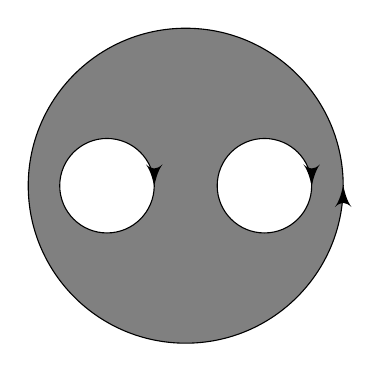
\begin{tikzpicture}
    \draw [fill = gray] circle [radius = 2];
    \draw [fill = white] (1, 0) circle [radius = 0.6];
    \draw [fill = white] (-1, 0) circle [radius = 0.6];
    \draw [->] (2, 0) -- (2, 0.01);
    \draw [->] (1.6, 0) -- (1.6, -0.01);
    \draw [->] (-0.4, 0) -- (-0.4, -0.01);
  \end{tikzpicture}
\end{center}
The orientation of the curve comes from imagining the surface as:
\begin{center}
  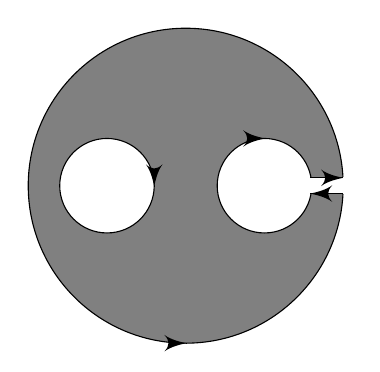
\begin{tikzpicture}
    \draw [fill = gray] circle [radius = 2];
    \draw [fill = white] (1, 0) circle [radius = 0.6];
    \draw [fill = white] (-1, 0) circle [radius = 0.6];
    \draw [->] (0, -2) -- (0.01, -2);
    \draw [->] (1, 0.6) -- (1.01, 0.6);
    \draw [->] (-0.4, 0) -- (-0.4, -0.01);
    \draw [fill = white, white] (1.5, 0.1) rectangle (2.1, -0.1);
    \draw [->] (2, -0.1) -- (1.58, -0.1);
    \draw [->] (1.58, 0.1) -- (2, 0.1);
  \end{tikzpicture}
\end{center}
and take the limit as the gap shrinks to 0.

\subsubsection{Stokes' theorem}
\begin{thm}[Stokes' theorem]
  For a smooth vector field $\mathbf{F}(\mathbf{r})$,
  \[
    \int_S \nabla\times \mathbf{F}\cdot \d \mathbf{S} = \int_{\partial S} \mathbf{F}\cdot \d \mathbf{r},
  \]
  where $S$ is a smooth, bounded surface and $\partial S$ is a piecewise smooth boundary of $S$.

  The direction of the line integral is as follows: If we walk along $C$ with $\mathbf{n}$ facing up, then the surface is on your left.
\end{thm}
It also holds if $\partial S$ is a collection of disconnected piecewise smooth closed curves, with the orientation determined in the same way as Green's theorem.

\begin{eg}
  Let $S$ be the section of a sphere of radius $a$ with $0 \leq \theta \leq \alpha$. In spherical coordinates,
  \[
    \d \mathbf{S} = a^2 \sin \theta \mathbf{e}_r \;\d \theta\;\d \varphi.
  \]
  Let $\mathbf{F} = (0, xz, 0)$. Then $\nabla \times \mathbf{F} = (-x, 0, z)$. We have previously shown that
  \[
    \int_S \nabla\times \mathbf{F}\cdot \d \mathbf{S} = \pi a^3 \cos\alpha\sin^2 \alpha.
  \]
  Our boundary $\partial C$ is
  \[
    \mathbf{r}(\varphi) = a(\sin \alpha\cos \alpha, \sin \alpha\sin \varphi, \cos \alpha).
  \]
  The right hand side of Stokes' is
  \begin{align*}
    \int_C \mathbf{F}\cdot \d \mathbf{r} &= \int_0^{2\pi}\underbrace{a\sin \alpha\cos \varphi}_{x}\underbrace{\vphantom{\varphi}a\cos\alpha}_z \underbrace{a\sin \alpha\cos\varphi\;\d \varphi}_{\d y}\\
    &= a^3\sin^2\alpha\cos\alpha\int_0^{2\pi}\cos^2\varphi\;\d \varphi\\
    &= \pi a^3\sin^2\alpha\cos\alpha.
  \end{align*}
  So they agree.
\end{eg}

\subsubsection{Divergence/Gauss theorem}
\begin{thm}[Divergence/Gauss theorem]
  For a smooth vector field $\mathbf{F}(\mathbf{r})$,
  \[
    \int _V \nabla\cdot \mathbf{F}\;\d V = \int_{\partial V}\mathbf{F}\cdot \d \mathbf{S},
  \]
  where $V$ is a bounded volume with boundary $\partial V$, a piecewise smooth, closed surface, with outward normal $\mathbf{n}$.
\end{thm}

\begin{eg}
  Consider a hemisphere.
  \begin{center}
    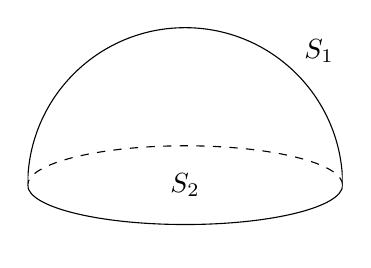
\begin{tikzpicture}
      \begin{scope}
        \clip (-2, 2) rectangle (2, 0);
        \draw circle [radius=2];
        \draw [dashed] circle [x radius = 2, y radius = 0.5];
      \end{scope}
      \begin{scope}
        \clip (-2, 0) rectangle (2, -0.7);
        \draw circle [x radius = 2, y radius = 0.5];
      \end{scope}
      \node {$S_2$};
      \node at (1.7, 1.7) {$S_1$};
    \end{tikzpicture}
  \end{center}

  $V$ is a solid hemisphere
  \[
    x^2 + y^2 + z^2 \leq a^2, \quad z \geq 0,
  \]
  and $\partial V = S_1 + S_2$, the hemisphere and the disc at the bottom.

  Take $\mathbf{F} = (0, 0, z + a)$ and $\nabla \cdot \mathbf{F} = 1$. Then
  \[
    \int_V\nabla \cdot \mathbf{F}\;\d V = \frac{2}{3}\pi a^3,
  \]
  the volume of the hemisphere.

  On $S_1$,
  \[
    \d \mathbf{S} = \mathbf{n}\;\d S = \frac{1}{a}(x, y, z)\;\d S.
  \]
  Then
  \[
    \mathbf{F}\cdot \d \mathbf{S} = \frac{1}{a}z(z + a)\;\d S = \cos \theta a(\cos \theta + 1)\underbrace{a^2\sin \theta\;\d \theta\;\d \varphi}_{\d S}.
  \]
  Then
  \begin{align*}
    \int_{S_1}\mathbf{F}\cdot \d \mathbf{S} &= a^3\int_0^{2\pi}\d \varphi \int_0^{\pi/2}\sin \theta(\cos^2\theta + \cos \theta)\;\d \theta\\
    &= 2\pi a^3 \left[\frac{-1}{3}\cos^3 \theta - \frac{1}{2}\cos^2 \theta\right]_0^{\pi/2}\\
    &= \frac{5}{3}\pi a^3.
  \end{align*}
  On $S_2$, $\d \mathbf{S} = \mathbf{n}\;\d S = -(0, 0, 1)\;\d S$. Then $\mathbf{F}\cdot \d \mathbf{S} = -a\;\d S$. So
  \[
    \int_{S_2} \mathbf{F}\cdot \d \mathbf{S} = -\pi a^3.
  \]
  So
  \[
    \int_{S_1}\mathbf{F}\cdot \d \mathbf{S} +\int_{S_2}\mathbf{F}\cdot \d \mathbf{S} = \left(\frac{5}{3} - 1\right)\pi a^3 = \frac{2}{3}\pi a^3,
  \]
  in accordance with Gauss' theorem.
\end{eg}

\subsection{Relating and proving integral theorems}
We will first show the following two equivalences:
\begin{itemize}
  \item Stokes' theorem $\Leftrightarrow $ Green's theorem
  \item 2D divergence theorem $\Leftrightarrow$ Greens' theorem
\end{itemize}
Then we prove the 2D version of divergence theorem directly to show that all of the above hold. A sketch of the proof of the 3D version of divergence theorem will be provided, because it is simply a generalization of the 2D version, except that the extra dimension makes the notation tedious and difficult to follow.

\begin{prop}
  Stokes' theorem $\Rightarrow $ Green's theorem
\end{prop}

\begin{proof}
  Stokes' theorem talks about 3D surfaces and Green's theorem is about 2D regions. So given a region $A$ on the $(x, y)$ plane, we pretend that there is a third dimension and apply Stokes' theorem to derive Green's theorem.

  Let $A$ be a region in the $(x, y)$ plane with boundary $C = \partial A$, parametrised by arc length, $(x(s), y(s), 0)$. Then the tangent to $C$ is
  \[
    \mathbf{t} = \left(\frac{\d x}{\d s}, \frac{\d y}{\d s}, 0\right).
  \]
  Given any $P(x, y)$ and $Q(x, y)$, we can consider the vector field
  \[
    \mathbf{F} = (P, Q, 0),
  \]
  So
  \[
    \nabla \times \mathbf{F} = \left(0, 0, \frac{\partial Q}{\partial x} - \frac{\partial P}{\partial y}\right).
  \]
  Then the left hand side of Stokes is
  \[
    \int_C \mathbf{F} \cdot \d \mathbf{r} = \int_C \mathbf{F}\cdot \mathbf{t}\;\d s = \int_C P\;\d x + Q\;\d y,
  \]
  and the right hand side is
  \[
    \int_A (\nabla\times \mathbf{F})\cdot \hat{\mathbf{k}}\;\d A = \int_A \left(\frac{\partial Q}{\partial x} - \frac{\partial P}{\partial y}\right)\;\d A.
  \]
\end{proof}

\begin{prop}
  Green's theorem $\Rightarrow $ Stokes' theorem.
\end{prop}

\begin{proof}
  Green's theorem describes a 2D region, while Stokes' theorem describes a 3D surface $\mathbf{r}(u, v)$. Hence to use Green's to derive Stokes' we need find some 2D thing to act on. The natural choice is the parameter space, $u, v$.

  Consider a parametrised surface $S = \mathbf{r}(u, v)$ corresponding to the region $A$ in the $u, v$ plane. Write the boundary as $\partial A = (u(t), v(t))$. Then $\partial S = \mathbf{r}(u(t), v(t))$.

  We want to prove
  \[
    \int_{\partial S}\mathbf{F}\cdot \d \mathbf{r} = \int_S (\nabla \times \mathbf{F})\cdot \d \mathbf{S}
  \]
  given
  \[
    \int_{\partial A} F_u\;\d u + F_v\;\d v = \int_A\left(\frac{\partial F_v}{\partial u} - \frac{\partial F_u}{\partial v}\right)\;\d A.
  \]
  Doing some pattern-matching, we want
  \[
    \mathbf{F}\cdot \d \mathbf{r} = F_u \;\d u + F_v \;\d v
  \]
  for some $F_u$ and $F_v$.

  By the chain rule, we know that
  \[
    \d \mathbf{r} = \frac{\partial \mathbf{r}}{\partial u} \d u + \frac{\partial \mathbf{r}}{\partial v}\d v.
  \]
  So we choose
  \[
    F_u = \mathbf{F}\cdot \frac{\partial \mathbf{r}}{\partial u}, \quad F_v = \mathbf{F}\cdot\frac{\partial \mathbf{r}}{\partial v}.
  \]
  This choice matches the left hand sides of the two equations.

  To match the right, recall that
  \[
    (\nabla\times \mathbf{F}) \cdot \d \mathbf{S} = (\nabla\times \mathbf{F})\cdot \left(\frac{\partial \mathbf{r}}{\partial u}\times \frac{\partial \mathbf{r}}{\partial v}\right).
  \]
  Therefore, for the right hand sides to match, we want
  \[
    \frac{\partial F_v}{\partial u} - \frac{\partial F_u}{\partial v} = (\nabla\times \mathbf{F})\cdot \left(\frac{\partial \mathbf{r}}{\partial u}\times \frac{\partial \mathbf{r}}{\partial v}\right).\tag{$*$}
  \]
  Fortunately, this is true. Unfortunately, the proof involves complicated suffix notation and summation convention:
  \[
    \frac{\partial F_v}{\partial u} = \frac{\partial}{\partial u}\left(\mathbf{F}\cdot \frac{\partial \mathbf{r}}{\partial v}\right) = \frac{\partial}{\partial u}\left(F_i\frac{\partial x_i}{\partial v}\right) = \left(\frac{\partial F_i}{\partial x_j}\frac{\partial x_j}{\partial u}\right)\frac{\partial x_i}{\partial v} + F_i\frac{\partial x_i}{\partial u\partial v}.
  \]
  Similarly,
  \[
    \frac{\partial F_u}{\partial u} = \frac{\partial}{\partial u}\left(\mathbf{F}\cdot \frac{\partial \mathbf{r}}{\partial u}\right) = \frac{\partial}{\partial u}\left(F_j\frac{\partial x_j}{\partial u}\right) = \left(\frac{\partial F_j}{\partial x_i}\frac{\partial x_i}{\partial v}\right)\frac{\partial x_j}{\partial u} + F_i\frac{\partial x_i}{\partial u\partial v}.
  \]
  So
  \[
    \frac{\partial F_v}{\partial u} - \frac{\partial F_u}{\partial v} = \frac{\partial x_j}{\partial u}\frac{\partial x_i}{\partial v}\left(\frac{\partial F_i}{\partial x_j} - \frac{\partial F_j}{\partial x_i}\right).
  \]
  This is the left hand side of $(*)$.

  The right hand side of $(*)$ is
  \begin{align*}
    (\nabla \times \mathbf{F})\cdot \left(\frac{\partial \mathbf{r}}{\partial u}\times \frac{\partial \mathbf{r}}{\partial v}\right) &= \varepsilon_{ijk}\frac{\partial F_j}{\partial x_i}\varepsilon_{kpq}\frac{\partial x_p}{\partial u}\frac{\partial x_q}{\partial v}\\
    &= (\delta_{ip}\delta_{jq} - \delta_{iq}\delta_{jp}) \frac{\partial F_j}{\partial x_i}\frac{\partial x_p}{\partial u}\frac{\partial x_q}{\partial v}\\
    &= \left(\frac{\partial F_j}{\partial x_i} - \frac{\partial F_i}{\partial x_j}\right)\frac{\partial x_i}{\partial u}\frac{\partial x_j}{\partial v}.
  \end{align*}
  So they match. Therefore, given our choice of $F_u$ and $F_v$, Green's theorem translates to Stokes' theorem.
\end{proof}


\begin{prop}
  Greens theorem $\Leftrightarrow$ 2D divergence theorem.
\end{prop}

\begin{proof}
  The 2D divergence theorem states that
  \[
    \int_A (\nabla\cdot \mathbf{G})\;\d A = \int_{\partial A} \mathbf{G}\cdot \mathbf{n}\;\d s.
  \]
  with an outward normal $\mathbf{n}$.

  Write $\mathbf{G}$ as $(Q, -P)$. Then
  \[
    \nabla\cdot \mathbf{G} = \frac{\partial Q}{\partial x} - \frac{\partial P}{\partial y}.
  \]
  Around the curve $\mathbf{r}(s) = (x(s), y(s))$, $\mathbf{t}(s) = (x'(s), y'(s))$. Then the normal, being tangent to $\mathbf{t}$, is $\mathbf{n}(s) = (y'(s), -x'(s))$ (check that it points outwards!). So
  \[
    \mathbf{G}\cdot \mathbf{n} = P\frac{\d x}{\d s} + Q\frac{\d y}{\d s}.
  \]
  Then we can expand out the integrals to obtain
  \[
    \int_C \mathbf{G}\cdot \mathbf{n}\;\d s = \int_C P\;\d x + Q\;\d y,
  \]
  and
  \[
    \int_A(\nabla\cdot \mathbf{G})\;\d A = \int_A\left(\frac{\partial Q}{\partial x} - \frac{\partial P}{\partial y}\right)\;\d A.
  \]
  Now 2D version of Gauss' theorem says the two LHS are the equal, and Green's theorem says the two RHS are equal. So the result follows.
\end{proof}

\begin{prop}
  2D divergence theorem.
  \[
    \int_A (\nabla\cdot \mathbf{G})\;\d A = \int_{C = \partial A} \mathbf{G}\cdot \mathbf{n}\;\d s.
  \]
\end{prop}

\begin{proof}
  For the sake of simplicity, we assume that $\mathbf{G}$ only has a vertical component, noting that the same proof works for purely horizontal $\mathbf{G}$, and an arbitrary $\mathbf{G}$ is just a linear combination of the two.

  Furthermore, we assume that $A$ is a simple, convex shape. A more complicated shape can be cut into smaller simple regions, and we can apply the simple case to each of the small regions.

  Suppose $\mathbf{G} = G(x, y)\hat{\mathbf{j}}$. Then
  \[
    \nabla \cdot \mathbf{G} = \frac{\partial G}{\partial y}.
  \]
  Then
  \[
    \int_A \nabla\cdot \mathbf{G}\;\d A = \int_X \left(\int_{Y_x}\frac{\partial G}{\partial y}\;\d y\right)\;\d x.
  \]
  Now we divide $A$ into an upper and lower part, with boundaries $C_+ = y_+(x)$ and $C_- = y_-(x)$ respectively. Since I cannot draw, $A$ will be pictured as a circle, but the proof is valid for any simple convex shape.
  \begin{center}
    \begin{tikzpicture}
      \draw [red] (3, 1.5) arc (0:180:1);
      \node [red, anchor = south east] at (1.2, 1.75) {$C_+$};
      \draw [blue] (1, 1.5) arc (180:360:1);
      \node [blue, anchor = north west] at (3, 1.5) {$C_-$};

      \draw (1.8, 0.52) -- (1.8, 2.48);
      \draw (2.2, 0.52) -- (2.2, 2.48);
      \draw [dashed] (1.8, 0.52) -- (1.8, 0);
      \draw [dashed] (2.2, 0.52) -- (2.2, 0);
      \node [below] at (2, 0) {$\d y$};

      \draw [dashed] (1.8, 0.52) -- (0, 0.52);
      \draw [dashed] (1.8, 2.48) -- (0, 2.48);
      \draw [->] (-0.3, 2.48) -- (-0.3, 0.52);
      \draw [->] (-0.3, 0.52) -- (-0.3, 2.48) node [pos = 0.5, fill=white] {$Y_x$};

      \draw [->] (0, 0) -- (5, 0) node [right] {$x$};
      \draw [->] (0, 0) -- (0, 3) node [above] {$y$};
    \end{tikzpicture}
  \end{center}
  We see that the boundary of $Y_x$ at any specific $x$ is given by $y_-(x)$ and $y_+(x)$. Hence by the Fundamental theorem of Calculus,
  \[
    \int_{Y_x}\frac{\partial G}{\partial y}\;\d y = \int_{y_-(x)}^{y_+(x)} \frac{\partial G}{\partial y}\;\d y = G(x, y_+(x)) - G(x, y_-(x)).
  \]
  To compute the full area integral, we want to integrate over all $x$. However, the divergence theorem talks in terms of $\d s$, not $\d x$. So we need to find some way to relate $\d s$ and $\d x$. If we move a distance $\delta s$, the change in $x$ is $\delta s\cos \theta$, where $\theta$ is the angle between the tangent and the horizontal. But $\theta$ is also the angle between the normal and the vertical. So $\cos \theta = \mathbf{n}\cdot \hat{\mathbf{j}}$. Therefore $\d x = \hat{\mathbf{j}}\cdot \mathbf{n}\;\d s$.

  In particular, $G\;\d x = G\,\hat{\mathbf{j}}\cdot \mathbf{n}\;\d s = \mathbf{G}\cdot \mathbf{n}\;\d s$, since $\mathbf{G} = G\,\hat{\mathbf{j}}$.

  However, at $C_-$, $\mathbf{n}$ points downwards, so $\mathbf{n}\cdot \hat{\mathbf{j}}$ happens to be negative. So, actually, at $C_-$, $\d x = -\mathbf{G}\cdot \mathbf{n}\;\d s$.

  Therefore, our full integral is
  \begin{align*}
    \int_A \nabla\cdot \mathbf{G}\;\d A &= \int_X \left(\int_{y_x}\frac{\partial G}{\partial y}\;\d Y\right)\;\d x\\
    &= \int_X G(x, y_+(x)) - G(x, y_{-}(x))\;\d x\\
    &= \int_{C_+}\mathbf{G}\cdot \mathbf{n}\;\d s + \int_{C_-}\mathbf{G}\cdot \mathbf{n}\;\d s\\
    &= \int_C \mathbf{G}\cdot \mathbf{n}\;\d s.
  \end{align*}
\end{proof}

To prove the 3D version, we again consider $\mathbf{F} = F(x, y, z)\hat{\mathbf{k}}$, a purely vertical vector field. Then
\[
  \int_V \nabla\cdot \mathbf{F}\;\d V = \int_D \left(\int_{Z_{xy}} \frac{\partial F}{\partial z}\;\d z\right)\;\d A.
\]
Again, split $S = \partial V$ into the top and bottom parts $S_+$ and $S_-$ (ie the parts with $\hat{\mathbf{k}}\cdot \mathbf{n} \geq 0$ and $\hat{\mathbf{k}}\cdot \mathbf{n} < 0$), and parametrize by $z_+(x, y)$ and $z_-(x, y)$. Then the integral becomes
\[
  \int_V \nabla\cdot \mathbf{F}\;\d V = \int_D (F(x, y, z_+) - F(x, y, z_-))\;\d A = \int_S \mathbf{F}\cdot \mathbf{n}\;\d S.
\]
\section{Some applications of integral theorems}
\subsection{Integral expressions for div and curl}
We can use these theorems to come up with alternative definitions of the div and curl. The advantage of these alternative definitions is that they do not require a choice of coordinate axes. They also better describe how we should interpret div and curl.

Gauss' theorem for $\mathbf{F}$ in a small volume $V$ containing $\mathbf{r}_0$ gives
\[
  \int_{\partial V}\mathbf{F}\cdot \d \mathbf{S} = \int_V\nabla\cdot \mathbf{F}\;\d V\approx (\nabla\cdot \mathbf{F})V.
\]
We take the limit as $V\to 0$ to obtain
\begin{prop}
  \[
    \nabla \cdot \mathbf{F} = \lim_{V \to 0} \frac{1}{V}\int_{\partial V}\mathbf{F}\cdot \d \mathbf{S}.
  \]
\end{prop}
Similarly, Stokes' gives
\[
  \int _{\partial A}\mathbf{F}\cdot \d \mathbf{r} = \int_A(\nabla\times \mathbf{F})\cdot \mathbf{n}\;\d A \approx \mathbf{n}\cdot (\nabla\times \mathbf{F})A.
\]
So
\begin{prop}
  \[
    \mathbf{n}\cdot \nabla \times \mathbf{F} = \lim_{A \to 0}\frac{1}{A}\int_{\partial A}\mathbf{F}\cdot \d \mathbf{r}.
  \]
\end{prop}
These are coordinate-independent definitions of div and curl.

\begin{eg}
  Suppose $\mathbf{u}$ is a velocity field of fluid flow. Then
  \[
    \int_S \mathbf{u}\cdot \d \mathbf{S}
  \]
  is the rate of which fluid crosses $S$. Taking $V$ to be the volume occupied by a fixed quantity of fluid material, we have
  \[
    \dot{V} = \int_{\partial V}\mathbf{u}\cdot \d \mathbf{S}
  \]
  Then, at $\mathbf{r}_0$,
  \[
    \nabla\cdot \mathbf{u} = \lim_{V\to 0}\frac{\dot{V}}{V},
  \]
  the relative rate of change of volume. For example, if $\mathbf{u}(\mathbf{r}) = \alpha\mathbf{r}$ (ie fluid flowing out of origin), then $\nabla\cdot \mathbf{u} = 3\alpha$, which increases at a constant rate everywhere.

  Alternatively, take a planar area $A$ to be a disc of radius $a$. Then
  \[
    \int_{\partial A}\mathbf{u}\cdot \d \mathbf{r} = \int_{\partial A}\mathbf{u}\cdot \mathbf{t} \;\d s = 2\pi a \times \text{average of $\mathbf{u}\cdot \mathbf{t}$ around the circumference}.
  \]
  ($\mathbf{u}\cdot \mathbf{t}$ is the component of $\mathbf{u}$ which is tangential to the boundary) We define the quantity
  \[
    \omega = \frac{1}{a} \times (\text{average of }\mathbf{u}\cdot \mathbf{t}).
  \]
  This is the local angular velocity of the current. As $a \to 0$, $\frac{1}{a} \to \infty$, but the average of $\mathbf{u}\cdot \mathbf{t}$ will also decrease since a smooth field is less ``twirly'' if you look closer. So $\omega$ tends to some finite value as $a\to 0$. We have
  \[
    \int_{\partial A} \mathbf{u}\cdot \d \mathbf{r} = 2\pi a^2 \omega.
  \]
  Recall that
  \[
    \mathbf{n}\cdot \nabla \times \mathbf{u} = \lim_{A \to 0}\frac{1}{\pi a^2}\int_{\partial A}\mathbf{u}\cdot \d \mathbf{r} = 2\omega,
  \]
  ie twice the local angular velocity. For example, if you have a washing machine rotating at a rate of $\boldsymbol\omega$, Then the velocity $\mathbf{u} = \boldsymbol\omega\times \mathbf{r}$. Then the curl is
  \[
    \nabla\times (\boldsymbol\omega\times \mathbf{r}) = 2\boldsymbol\omega,
  \]
  which is twice the angular velocity.
\end{eg}

\subsection{Conservative fields and scalar products}
\begin{defi}[Conservative field]
  A vector field $\mathbf{F}$ is \emph{conservative} if
  \begin{enumerate}
    \item $\mathbf{F} = \nabla f$ for some scalar field $f$; or
    \item $\int_C \mathbf{F}\cdot \d \mathbf{r}$ is independent of $C$, for fixed end points and orientation; or
    \item $\nabla \times \mathbf{F} = 0$.
  \end{enumerate}
  In $\R^3$, all three formulations are equivalent.
\end{defi}

We have previously shown (i) $\Rightarrow$ (ii) since
\[
  \int_C \mathbf{F}\cdot \d \mathbf{r} = f(\mathbf{b}) - f(\mathbf{a}).
\]
We have also shown that (i) $\Rightarrow$ (iii) since
\[
  \nabla \times (\nabla f) = 0.
\]
So we want to show that (iii) $\Rightarrow $ (ii) and (ii) $\Rightarrow $ (i)
\begin{prop}
  If (iii) $\nabla\times \mathbf{F}= 0 $, then (ii) $\int_C \mathbf{F}\cdot \d \mathbf{r}$ is independent of $C$.
\end{prop}

\begin{proof}
  Given $\mathbf{F}(\mathbf{r})$ satisfying $\nabla\times \mathbf{F} = 0$, let $C$ and $\tilde C$ be any two curves from $\mathbf{a}$ to $\mathbf{b}$.
  \begin{center}
    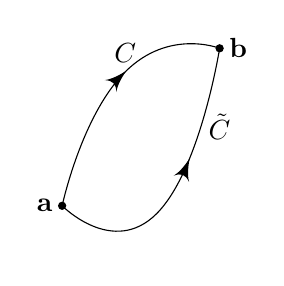
\begin{tikzpicture}
      \node [circ] {};
      \node [left] {$\mathbf{a}$};
      \node at (2, 2) [circ] {};
      \node at (2, 2) [right] {$\mathbf{b}$};
      \node at (2, 1) {$\tilde C$};
      \draw [->-=0.6] plot [smooth, tension=1] coordinates {(0, 0) (0.8, 1.7) (2, 2)};
      \node [above] at (0.8, 1.7) {$C$};
      \draw [->-=0.6] plot [smooth, tension=1] coordinates {(0, 0) (1.2, -0.1) (2, 2)};
    \end{tikzpicture}
  \end{center}
  If $S$ is any surface with boundary $\partial S = C - \tilde C$, By Stokes' theorem,
  \[
    \int_{S}\nabla \times \mathbf{F}\cdot \d \mathbf{S} = \int_{\partial S}\mathbf{F}\cdot \d \mathbf{r} = \int_C \mathbf{F}\cdot \d \mathbf{r} - \int_{\tilde{C}}\mathbf{F}\cdot \d \mathbf{r}.
  \]
  But $\nabla\times \mathbf{F} = 0$. So
  \[
    \int_C \mathbf{F}\cdot \d \mathbf{r} - \int_{\tilde{C}} \mathbf{F}\cdot \d \mathbf{r} = 0,
  \]
  or
  \[
    \int_C \mathbf{F}\cdot \d \mathbf{r} = \int_{\tilde{C}}\mathbf{F}\cdot \d \mathbf{r}.
  \]
\end{proof}

\begin{prop}
  If (ii) $\int_C \mathbf{F}\cdot \d \mathbf{r}$ is independent of $C$ for fixed end points and orientation, then (i) $\mathbf{F} = \nabla f$ for some scalar field $f$.
\end{prop}

\begin{proof}
  We fix $\mathbf{a}$ and define $f(\mathbf{r}) = \int_C \mathbf{F}(\mathbf{r}')\cdot\d \mathbf{r}'$ for any curve from $\mathbf{a}$ to $\mathbf{r}$. Assuming (ii), $f$ is well-defined. For small changes $\mathbf{r}$ to $\mathbf{r} + \delta \mathbf{r}$, there is a small extension of $C$ by $\delta C$. Then
  \begin{align*}
    f(\mathbf{r} + \delta \mathbf{r}) &= \int_{C + \delta C}\mathbf{F} (\mathbf{r}')\cdot \d \mathbf{r}'\\
    &= \int_C \mathbf{F}\cdot \d \mathbf{r}' + \int_{\delta C}\mathbf{F}\cdot \d \mathbf{r}'\\
    &= f(\mathbf{r}) + \mathbf{F}(\mathbf{r})\cdot \delta \mathbf{r} + o(\delta \mathbf{r}).
  \end{align*}
  So
  \[
    \delta f = f(\mathbf{r} + \delta \mathbf{r}) - f(\mathbf{r}) = \mathbf{F}(\mathbf{r})\cdot \delta \mathbf{r} + o(\delta \mathbf{r}).
  \]
  But the definition of grad is exactly
  \[
    \delta f = \nabla f\cdot \delta \mathbf{r} + o(\delta \mathbf{r}).
  \]
  So we have $\mathbf{F} = \nabla f$.
\end{proof}
Note that these results assume $\mathbf{F}$ is defined on the whole of $\R^3$. It also works of $\mathbf{F}$ is defined on a \emph{simply connected} domain $D$, ie a subspace of $\R^3$ without holes. By definition, this means that any two curves $C, \tilde{C}$ with fixed end points can be smoothly deformed into one another (alternatively, any loop can be shrunk into a point).

If we have a smooth transformation from $C$ to $\tilde{C}$, the process sweeps out a surface bounded by $C$ and $\tilde{C}$. This is required by the proof that (iii) $\Rightarrow$ (ii).

If $D$ is not simply connected, then we obtain a multi-valued $f(\mathbf{r})$ on $D$ in general (for the proof (ii) $\Rightarrow$ (i)). However, we can choose to restrict to a subset $D_0\subseteq D$ such that $f(\mathbf{r})$ is single-valued on $D_0$.

\begin{eg}
  Take
  \[
    \mathbf{F} = \left(\frac{- y}{x^2 + y^2}, \frac{x}{x^2 + y^2}, 0\right).
  \]
  This obeys $\nabla\times \mathbf{F} = 0$, and is defined on $D = \R^3 \setminus \{z\text{-axis}\}$, which is not simply-connected. We can also write
  \[
    \mathbf{F} = \nabla f,
  \]
  where
  \[
    f = \tan^{-1}\frac{y}{x}.
  \]
  which is multi-valued. If we integrate it about the closed loop $x^2 + y^2 = 1, z = 0$, ie. a circle about the $z$ axis, the integral gives $2\pi$, as opposed to the expected $0$ for a conservative force. This shows that the simply-connected-domain criterion is important!

  However $f$ can be single-valued if we restrict it to
  \[
    D_0 = \R^3 - \{\text{half-plane }x \geq 0,\, y = 0\},
  \]
  which is simply-connected. (Draw and check!) Any closed curve we can draw in this area will have an integral of $0$ (the circle mentioned above will no longer be closed!).
\end{eg}

\subsection{Conservation laws}
\begin{defi}[Conservation equation]
  Suppose we are interested in a quantity $Q$. Let $\rho(\mathbf{r}, t)$ be the amount of stuff per unit volume and $\mathbf{j}(\mathbf{r}, t)$ be the flow rate of the quantity (eg if $Q$ is charge, $j$ is the current density).

  The conservation equation is
  \[
    \frac{\partial \rho}{\partial t} + \nabla\cdot \mathbf{j} = 0.
  \]
\end{defi}
This is stronger than the claim that the total amount of $Q$ in the universe is fixed. It says that $Q$ cannot just disappear here and appear elsewhere. It must continuously flow out.

In particular, let $V$ be a fixed time-independent volume with boundary $S = \partial V$. Then
\[
  Q(t) = \int_V \rho (\mathbf{r}, t)\; \d V
\]
Then the rate of change of amount of $Q$ in $V$ is
\[
  \frac{\d Q}{\d t} = \int_V \frac{\partial \rho }{\partial t}\;\d V = -\int_V \nabla \cdot \mathbf{j}\;\d V = -\int_S \mathbf{j}\cdot \d \mathbf{s}.
\]
by divergence theorem. So this states that the rate of change of the quantity $Q$ in $V$ is the flux of the stuff flowing out of the surface. ie $Q$ cannot just disappear but must smoothly flow out.

In particular, if $V$ is the whole universe (ie $\R^3$), and $\mathbf{j}\to 0$ sufficiently rapidly as $|\mathbf{r}| \to \infty$, then we calculate the total amount of $Q$ in the universe by taking $V$ to be a solid sphere of radius $R$, and take the limit as $R\to \infty$. Then the surface integral $\to 0$, and the equation states that
\[
  \frac{\d Q}{\d t} = 0,
\]
\begin{eg}
  If $\rho(\mathbf{r}, t)$ is the charge density (ie. $\rho\delta V$ is the amount of charge in a small volume $\delta V$), then $Q(t)$ is the total charge in $V$. $\mathbf{j}(\mathbf{r}, t)$ is the electric current density. So $\mathbf{j}\cdot \d \mathbf{S}$ is the charge flowing through $\delta S$ per unit time.
\end{eg}

\begin{eg}
  Let $\mathbf{j} = \rho \mathbf{u}$ with $\mathbf{u}$ being the velocity field. Then $(\rho\mathbf{u}\; \delta t)\cdot \delta \mathbf{S}$ is equal to the mass of fluid crossing $\delta S$ in time $\delta t$. So
  \[
    \frac{\d Q}{\d t} = -\int_S \mathbf{j}\cdot \d \mathbf{S}
  \]
  does indeed imply the conservation of mass. The conservation equation in this case is
  \[
    \frac{\partial \rho}{\partial t} + \nabla\cdot (\rho \mathbf{u}) = 0
  \]
  For the case where $\rho$ is constant and uniform (ie. independent of $\mathbf{r}$ and $t$), we get that $\nabla\cdot \mathbf{u} = 0$. We say that the fluid is \emph{incompressible}.
\end{eg}

\section{Orthogonal curvilinear coordinates}
\subsection{Line, area and volume elements}
In this chapter, we study funny coordinate systems. A coordinate system is, roughly speaking, a way to specify a point in space by a set of (usually 3) numbers. We can think of this as a function $\mathbf{r}(u, v, w)$.

By the chain rule, we have
\[
  \d \mathbf{r} = \frac{\partial \mathbf{r}}{\partial u}\d u + \frac{\partial \mathbf{r}}{\partial v}\d v + \frac{\partial \mathbf{r}}{\partial w}\d w
\]
For a good parametrization,
\[
  \frac{\partial \mathbf{r}}{\partial u}\cdot \left(\frac{\partial \mathbf{r}}{\partial v}\times \frac{\partial \mathbf{r}}{\partial w}\right) \not = 0,
\]
ie. $\frac{\partial \mathbf{r}}{\partial u}, \frac{\partial \mathbf{r}}{\partial v}$ and $\frac{\partial \mathbf{r}}{\partial w}$ are linearly independent. These vectors are tangent to the curves parametrized by $u, v, w$ respectively when the other two are being fixed.

Even better, they should be orthogonal:
\begin{defi}[Orthogonal curvilinear coordinates]
  $u, v, w$ are \emph{orthogonal curvilinear} if the tangent vectors are orthogonal.
\end{defi}
We can then set
\[
  \frac{\partial \mathbf{r}}{\partial u} = h_u \mathbf{e}_u, \quad \frac{\partial \mathbf{r}}{\partial v} = h_v \mathbf{e}_v,\quad \frac{\partial \mathbf{r}}{\partial w} = h_w \mathbf{e}_w,
\]
with $h_u, h_v, h_w > 0$ and $\mathbf{e}_u, \mathbf{e}_v, \mathbf{e}_w$ form an \emph{orthonormal} right-handed basis (ie. $\mathbf{e}_u \times \mathbf{e}_v = \mathbf{e}_w$). Then
\[
  \d \mathbf{r} = h_u \mathbf{e}_u \;\d u + h_v \mathbf{e}_v\;\d v + h_w\mathbf{e}_w \;\d w,
\]
and $h_u, h_v, h_w$ determine the changes in length along each orthogonal direction resulting from changes in $u, v, w$. Note that clearly by definition, we have
\[
  h_u = \left|\frac{\partial \mathbf{r}}{\partial u}\right|.
\]
\begin{eg}\leavevmode
  \begin{enumerate}
    \item In cartesian coordinates, $\mathbf{r}(x, y, z) = x\hat{\mathbf{i}} + y\hat{\mathbf{j}} + z\hat{\mathbf{k}}$. Then $h_x = h_y = h_z = 1$, and $\mathbf{e}_x = \hat{\mathbf{i}}, \mathbf{e}_y = \hat{\mathbf{j}}$ and $\mathbf{e}_z = \hat{\mathbf{k}}$.
    \item In cylindrical polars, $\mathbf{r}(\rho, \varphi, z) = \rho[\cos \varphi\hat{\mathbf{i}} + \sin \varphi \hat{\mathbf{j}}] + z \hat{\mathbf{k}}$. Then $h_\rho = h_z = 1$, and
      \[
        h_\varphi = \left|\frac{\partial \mathbf{r}}{\partial \varphi}\right| = |(-\rho \sin\varphi, \rho \sin \varphi, 0)| = \rho.
      \]
      The basis vectors $\mathbf{e}_\rho, \mathbf{e}_\varphi, \mathbf{e}_z$ are as in section 1.
    \item In spherical polars,
      \[
        \mathbf{r}(r, \theta, \varphi) = r(\cos \varphi\sin \theta\hat{\mathbf{i}} + \sin \theta\sin \varphi\hat{\mathbf{j}} + \cos \theta \hat{\mathbf{k}}).
      \]
      Then $h_r = 1, h_\theta = r$ and $h_\varphi = r\sin \theta$.
  \end{enumerate}
\end{eg}

Consider a surface with $w$ constant and parametrised by $u$ and $v$. The vector area element is
\[
  \d \mathbf{S} = \frac{\d \mathbf{r}}{\partial u}\times \frac{\partial \mathbf{r}}{\partial v}\;\d u\;\d v = h_u \mathbf{e}_u \times h_v \mathbf{e}_v \;\d u\;\d v = h_uh_v \mathbf{e}_w \;\d u\;\d v.
\]
We interpret this as $\delta S$ having a small rectangle with sides approximately $h_u \delta u$ and $h_v \delta v$. The volume element is
\[
  \d V = \frac{\partial \mathbf{r}}{\partial u}\cdot \left(\frac{\partial \mathbf{r}}{\partial v}\times \frac{\partial \mathbf{r}}{\partial w}\right)\;\d u\;\d v\;\d w = h_uh_vh_w \;\d u\;\d v\;\d w,
\]
ie. a small cuboid with sides $h_u \delta _u$, $h_v\delta _v$ and $h_w \delta_w$ respectively.

\subsection{Grad, Div and Curl}
Consider $f(\mathbf{r}(u, v, w))$ and compare
\[
  \d f = \frac{\partial f}{\partial u}\;\d u + \frac{\partial f}{\partial v}\;\d v + \frac{\partial f}{\partial w}\;\d w,
\]
with $\d f = (\nabla f)\cdot \d \mathbf{r}$. Since we know that
\[
  \d \mathbf{r} = \frac{\partial \mathbf{r}}{\partial u}\;\d u + \frac{\partial \mathbf{r}}{\partial v}\;\d v + \frac{\partial \mathbf{r}}{\partial w}\;\d w = h_u \mathbf{e}_u \;\d u + h_v \mathbf{e}_v \;\d v + h_w \mathbf{e}_w \;\d v,
\]
we can compare the terms to know that
\begin{prop}
  \[
    \nabla f = \frac{1}{h_u} \frac{\partial f}{\partial u} \mathbf{e}_u + \frac{1}{h_v} \frac{\partial f}{\partial v}\mathbf{e}_v + \frac{1}{h_w} \frac{\partial f}{\partial w}\mathbf{e}_w.
  \]
\end{prop}
\begin{eg}
  Take $f = r\sin \theta\cos \varphi$ in spherical polars. Then
  \begin{align*}
    \nabla f &= \sin \theta\cos \varphi\,\mathbf{e}_r + \frac{1}{r}(r\cos \theta\cos \varphi)\,\mathbf{e}_\theta + \frac{1}{r\sin \theta}(-r\sin \theta\sin \varphi)\,\mathbf{e}_\varphi\\
    &= \cos\varphi(\sin \theta \,\mathbf{e}_r + \cos \theta \,\mathbf{e}_\theta) - \sin \varphi \,\mathbf{e}_\varphi.
  \end{align*}
\end{eg}

Then we know that the differential operator is
\begin{prop}
  \[
    \nabla = \frac{1}{h_u}\mathbf{e}_u \frac{\partial }{\partial u} + \frac{1}{h_v}\mathbf{e}_v\frac{\partial }{\partial v} + \frac{1}{h_w}\mathbf{e}_w \frac{\partial}{\partial w}.
  \]
\end{prop}
We can apply this to a vector field
\[
  \mathbf{F} = F_u \mathbf{e}_u + F_v \mathbf{e}_v + F_w \mathbf{e}_w
\]
using scalar or vector products to obtain
\begin{prop}
  \begin{align*}
    \nabla \times \mathbf{F} &= \frac{1}{h_vh_w}\left[\frac{\partial}{\partial v}(h_wF_w) - \frac{\partial }{\partial w}(h_vF_v)\right]\mathbf{e}_u + \text{ two similar terms}\\
    &= \frac{1}{h_uh_vh_w}
    \begin{vmatrix} h_u\mathbf{e}_u & h_v\mathbf{e}_v & h_w \mathbf{e}_w\\
      \frac{\partial}{\partial u} & \frac{\partial}{\partial v} & \frac{\partial}{\partial w}\\
      h_u f_u & h_v F_v & h_wF_w
    \end{vmatrix}
  \end{align*}
  and
  \[
    \nabla\cdot \mathbf{F} = \frac{1}{h_uh_vh_w}\left[\frac{\partial}{\partial u}(h_vh_wF_u) + \text{ two similar terms}\right].
  \]
\end{prop}
There are several ways to obtain these formulae. We can

\begin{proof}(non-examinable)
  \begin{enumerate}
    \item Apply $\nabla\cdot$ or $\nabla\times$ and differentiate the basis vectors explicitly.
    \item First, apply $\nabla\cdot$ or $\nabla\times$, but calculate the result by writing $\mathbf{F}$ in terms of $\nabla \mathbf{u}, \nabla \mathbf{v}$ and $\nabla \mathbf{w}$ in a suitable way. Then use $\nabla\times \nabla f = 0$ and $\nabla\cdot (\nabla\times f) = 0$.
    \item Use the integral expressions for div and curl.

      Recall that
      \[
        \mathbf{n}\cdot \nabla \times \mathbf{F} = \lim_{A \to 0}\frac{1}{A}\int_{\partial A}\mathbf{F}\cdot \d \mathbf{r}.
      \]
      So to calculate the curl, we first find the $\mathbf{e}_w$ component.

      Consider an area with $W$ fixed and change $u$ by $\delta u$ and $v$ by $\delta v$. Then this has an area of $h_u h_v \delta u\delta v$ with normal $\mathbf{e}_w$. Let $C$ be its boundary.
      \begin{center}
        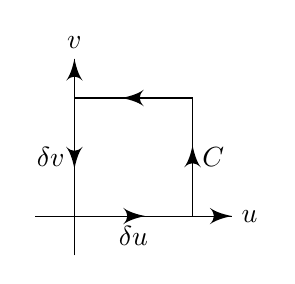
\begin{tikzpicture}
          \draw [->] (-0.5, 0) -- (2, 0) node [right] {$u$} node [pos = 0.5, below] {$\delta u$};
          \draw [->] (0, -0.5) -- (0, 2) node [above] {$v$} node [pos = 0.5, left] {$\delta v$};
          \draw [->-=0.6] (1.5, 0) -- (1.5, 1.5) node [pos = 0.5, right] {$C$};
          \draw [->-=0.6] (1.5, 1.5) -- (0, 1.5);
          \draw [->-=0.6] (0, 1.5) -- (0, 0);
          \draw [->-=0.6] (0, 0) -- (1.5, 0);
        \end{tikzpicture}
      \end{center}
      We then integrate around the curve $C$. We split the curve $C$ up into 4 parts (corresponding to the four sides), and take linear approximations by assuming $F$ and $h$ are constant when moving through each horizontal/vertical segment.
      \begin{align*}
        \int_C \mathbf{F}\cdot \d \mathbf{r} &\approx F_u(u, v) h_u(u, v)\;\delta u + F_v(u + \delta u, v) h_v(u + \delta u, v)\;\delta u \\
        &- F_u(u, v + \delta v)h_u (u, v + \delta v)\; \delta u - F_v(u, v)h_v(u, v)\;\delta v\\
        &\approx \left[\frac{\partial}{\partial u}h_vF_v - \frac{\partial}{\partial v}(h_uF_u)\right]\delta u\delta v.
      \end{align*}
      Divide by the area and take the limit as area $\to 0$, we obtain
      \[
        \lim_{A \to 0} \frac{1}{A}\int_C \mathbf{F}\cdot \d \mathbf{r} = \frac{1}{h_uh_v}\left[\frac{\partial}{\partial u}h_vF_v - \frac{\partial}{\partial v}(h_u F_u)\right].
      \]
      So, by the integral definition of divergence,
      \[
        \mathbf{e}_w\cdot \nabla\times \mathbf{F} = \frac{1}{h_uh_v}\left[\frac{\partial }{\partial u}(h_vF_v) - \frac{\partial }{\partial v}(h_uF_u)\right],
      \]
      and similarly for other components.

      We can find the divergence similarly.
  \end{enumerate}
\end{proof}

\begin{eg}
  Let $\mathbf{A} = \frac{1}{r}\tan \frac{\theta}{2} \mathbf{e}_\varphi$ in spherical polars. Then
  \[
    \nabla\times \mathbf{A} = \frac{1}{r^2\sin \theta}
    \begin{vmatrix}
      \mathbf{e}_r & r\mathbf{e}_\theta & r\sin \theta \mathbf{e}_\varphi\\
      \frac{\partial}{\partial r} & \frac{\partial}{\partial \theta} & \frac{\partial}{\partial \varphi}\\
      0 & 0 & r\sin \theta \cdot \frac{1}{r}\tan \frac{\theta}{2}
    \end{vmatrix} = \frac{\mathbf{e}_r}{r^2\sin \theta}\frac{\partial}{\partial \theta}\left[\sin \theta\tan \frac{\theta}{2}\right] = \frac{1}{r^2}\mathbf{e}_r.
  \]
\end{eg}

\section{Gauss' Law and Poisson's equation}
\subsection{Laws of gravitation}
Consider a distribution of mass producing a gravitational force $\mathbf{F}$ on a point mass $m$ at $\mathbf{r}$. The total force is a sum of contributions from each part of the mass distribution, and is proportional to $m$. Write
\[
  \mathbf{F} = m\mathbf{g}(\mathbf{r}),
\]
\begin{defi}[Gravitational field]
  $\mathbf{g}(\mathbf{r})$ is the \emph{gravitational field}, \emph{acceleration due to gravity}, or \emph{force per unit mass}.
\end{defi}
The gravitational field is conservative, ie
\[
  \oint_C \mathbf{g}\cdot \d \mathbf{r} = 0.
\]
This means that if you walk around the place and return to the same position, the total work done is $0$ and you did not gain energy, ie. gravitational potential energy is conserved.

Gauss' law tells us what this gravitational field looks like:
\begin{law}[Gauss' law for gravitation]
  Given any volume $V$ bounded by closed surface $S$,
  \[
    \int_S \mathbf{g}\cdot \d \mathbf{S} = -4\pi GM,
  \]
  where $G$ is Newton's gravitational constant, and $M$ is the total mass contained in $V$.
\end{law}
These equations determine $\mathbf{g}(\mathbf{r})$ from a mass distribution.

\begin{eg}
  We can obtain Newton's law of gravitation from Gauss' law together with an assumption about symmetry.

  Consider a total mass $M$ distributed with a spherical symmetry about the origin $\mathbf{O}$, with all the mass contained within some radius $r = a$. By spherical symmetry, we have $\mathbf{g}(\mathbf{r}) = g(\mathbf{r})\hat{\mathbf{r}}$.

  Consider Gauss' law with $S$ being a sphere of radius $r = R > a$. Then $\hat{\mathbf{n}} = \hat{\mathbf{r}}$. So
  \[
    \int_S \mathbf{g}\cdot \d \mathbf{S} = \int_S g(R)\hat{\mathbf{r}}\cdot \hat{\mathbf{r}}\;\d S = \int g(R)\d S = 4\pi R^2 g(R).
  \]
  By Gauss' law, we obtain
  \[
    4\pi R^2 g(R) = -4\pi GM.
  \]
  So
  \[
    g(R) = -\frac{GM}{R^2}
  \]
  for $R > a$.

  Therefore the gravitational force on a mass $m$ at $\mathbf{r}$ is
  \[
    \mathbf{F}(\mathbf{r}) = -\frac{GMm}{r^2}\hat{\mathbf{r}}.
  \]
  If we take the limit as $a\to 0$, we get a point mass $M$ at the origin. Then we recover Newton's law of gravitation for point masses.
\end{eg}

The condition $\int_C \mathbf{g}\cdot \d \mathbf{r} = 0$ for any closed $C$ can be re-written by Stoke's theorem as
\[
  \int_S \nabla\times \mathbf{g}\cdot \d \mathbf{S} = 0,
\]
where $S$ is bounded by the closed curve $C$. This is true for arbitrary $S$. So
\[
  \nabla\times \mathbf{g} = 0.
\]
In our example above, $\nabla\times \mathbf{g} = 0$ due to spherical symmetry. But here we showed that it is true for all cases.

Note that we exploited symmetry to solve Gauss' law. However, if the mass distribution is not sufficiently symmetrical, Gauss' law in integral form can be difficult to use. But we can rewrite it in differential form. Suppose
\[
  M = \int_V \rho(\mathbf{r})\;\d V,
\]
where $\rho$ is the mass density. Then by Gauss' theorem
\[
  \int_S \mathbf{g} \cdot \d \mathbf{S} = -4\pi GM \Rightarrow \int_V \nabla\cdot \mathbf{g}\;\d V = \int_V -4\pi G\rho \;\d V.
\]
Since this is true for all $V$, we must have
\begin{law}[Gauss' Law for gravitation in differential form]
  \[
    \nabla\cdot \mathbf{g} = -4\pi G\rho.
  \]
\end{law}
Since $\nabla\times \mathbf{g} = 0$, we can introduce a gravitational potential $\varphi(\mathbf{r})$ with $\mathbf{g} = -\nabla \varphi$. Then Gauss' Law becomes
\[
  \nabla^2 \varphi = 4\pi G\rho.
\]
In the example with spherical symmetry, we can solve that
\[
  \varphi(r) = -\frac{GM}{r}
\]
for $r > a$.
\subsection{Laws of electrostatics}
Consider a distribution of electric charge at rest. They produce a force on a charge $q$, at rest at $\mathbf{r}$, which is proportional to $q$.
\begin{defi}[Electric field]
  The force produced by electric charges on another charge $q$ is $\mathbf{F} = q\mathbf{E}(\mathbf{r})$, where $\mathbf{E}(\mathbf{r})$ is the \emph{electric field}, or force per unit charge.
\end{defi}
Again, this is conservative. So
\[
  \oint_C \mathbf{E}\cdot \d \mathbf{r} = 0
\]
for any closed curve $C$. It also obeys
\begin{law}[Gauss' law for electrostatic forces]
  \[
    \int_S \mathbf{E}\cdot \d \mathbf{S} = \frac{Q}{\varepsilon_0},
  \]
  where $\varepsilon_0$ is the \emph{permittivity of free space}, or \emph{electric constant}.
\end{law}

Then we can write it in differential form, as in the gravitational case.
\begin{law}[Gauss' law for electrostatic forces in differential form]
  \[
    \nabla \cdot \mathbf{E} = \frac{\rho}{\varepsilon_0}.
  \]
\end{law}
Assuming constant (or no) magnetic field, we have
\[
  \nabla\times \mathbf{E} = 0.
\]
So we can write $\mathbf{E} =- \nabla \varphi$.
\begin{defi}[Electrostatic potential]
  If we write $\mathbf{E} = -\nabla \varphi$, then $\varphi$ is the \emph{electrostatic potential}, and
  \[
    \nabla^2 \varphi = \frac{\rho}{\varepsilon_0}.
  \]
\end{defi}

\begin{eg}
  Take a spherically symmetric charge distribution about $O$ with total charge $Q$. Suppose all charge is contained within a radius $r = a$. Then similar to the gravitational case, we have
  \[
    \mathbf{E}(\mathbf{r}) = \frac{Q\hat{\mathbf{r}}}{4\pi \varepsilon_0 r^2},
  \]
  and
  \[
    \varphi(\mathbf{r}) = \frac{-Q}{4\pi\varepsilon_0 r}.
  \]
  As $a \to 0$, we get \emph{point charges}. From $\mathbf{E}$, we can recover Coulomb's law for the force on another charge $q$ at $\mathbf{r}$:
  \[
    \mathbf{F} = q\mathbf{E} =\frac{qQ\hat{\mathbf{r}}}{4\pi \varepsilon_0 r^2}.
  \]
\end{eg}

\begin{eg}[Line charge]
  Consider an infinite line with uniform charge density \emph{per unit length} $\sigma$.

  We use cylindrical polar coordinates:
  \begin{center}
    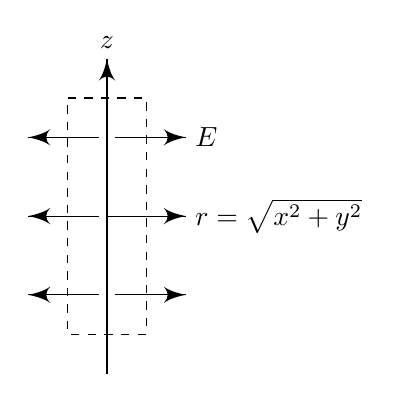
\begin{tikzpicture}
      \draw [->] (0, -2) -- (0, 2) node [above] {$z$};
      \draw [->] (0, 0) -- (1, 0) node [right] {$r = \sqrt{x^2 + y^2}$};

      \draw [->] (0.1, 1) -- (1, 1) node [right] {$E$};
      \draw [->] (-0.1, 1) -- (-1, 1);
      \draw [->] (-0.1, 0) -- (-1, 0);
      \draw [->] (0.1, -1) -- (1, -1);
      \draw [->] (-0.1, -1) -- (-1, -1);

      \draw [dashed] (-0.5, 1.5) -- (0.5, 1.5) -- (0.5, -1.5) -- (-0.5, -1.5) -- cycle;
    \end{tikzpicture}
  \end{center}
  By symmetry, the field is radial, ie.
  \[
    \mathbf{E}(r) = E(r) \hat{\mathbf{r}}.
  \]
  Pick $S$ to be a cylinder of length $L$ and radius $r$. We know that the end caps do not contribute to the flux since the field lines are perpendicular to the normal. Also, the curved surface has area $2\pi r L$. Then by Gauss' law in integral form,
  \[
    \int_S\mathbf{E}\cdot \d \mathbf{S} = E(r)2\pi rL = \frac{\sigma L}{\varepsilon_0}.
  \]
  So
  \[
    \mathbf{E}(r) = \frac{\sigma}{2\pi \varepsilon_0 r} \hat{\mathbf{r}}.
  \]
  Note that the field varies as $1/r$, not $1/r^2$. Intuitively, this is because we have one more dimension of ``stuff'' compared to the point charge, so the field does not drop as fast.
\end{eg}

\subsection{Poisson's Equation and Laplace's equation}
\begin{defi}[Poisson's equation]
  The \emph{Poisson's equation} is
  \[
    \nabla^2 \varphi = -\rho,
  \]
  where $\rho$ is given and $\varphi(\mathbf{r})$ is to be solved.
\end{defi}
This is the form of the equations for gravity and electrostatics, with $-4\pi G \rho$ and $\rho/\varepsilon_0$ in place of $\rho$ respectively.

When $\rho = 0$, we get
\begin{defi}[Laplace's equation]
  Laplace's equation is
  \[
    \nabla^2 \varphi = 0.
  \]
\end{defi}
One example is irrotational and incompressible fluid flow: if the velocity is $\mathbf{u}(\mathbf{r})$, then irrotationality gives $\mathbf{u} = \nabla \varphi$ for some \emph{velocity potential} $\varphi$. Since it is incompressible, $\nabla\cdot \mathbf{u} = 0$ (cf. previous chapters). So $\nabla^2 \varphi = 0$.

The expressions for $\nabla^2$ can be found in non-Cartesian coordinates, but are a bit complicated.

We're concerned here mainly with cases exhibiting spherical or cylindrical symmetry (use $r$ for radial coordinate here). ie. when $\varphi(\mathbf{r})$ has spherical or cylindrical symmetry. Write $\varphi = \varphi(r) \hat{\mathbf{r}}$. Then
\[
  \nabla \varphi = \varphi'(r)\hat{\mathbf{r}}.
\]
Then Laplace's equation $\nabla^2 \varphi = 0$ becomes an ordinary differential equation.
\begin{itemize}
  \item For spherical symmetry, using the chain rule, we have
    \[
      \nabla^2 \varphi = \varphi'' + \frac{2}{r}\varphi' = \frac{1}{r^2}(r^2\varphi')' = 0.
    \]
    Then the general solution is
    \[
      \varphi = \frac{A}{r} + B.
    \]
  \item For cylindrical symmetry, with $r^2 = x_1^2 + x_2^2$, we have
    \[
      \nabla^2 \varphi = \varphi'' + \frac{1}{r}\varphi' = \frac{1}{r}(r\varphi')' = 0.
    \]
    Then
    \[
      \varphi = A\ln r + B.
    \]
\end{itemize}
Then solutions to Poisson's equations can be obtained in a similar way, ie. by integrating the differential equations directly, or by adding particular integrals to the solutions above.

For example, for a spherically symmetric solution of $\nabla^2 \varphi = -\rho_0$, with $\rho_0$ constant, recall that $\nabla^2 r^\alpha = \alpha(\alpha + 1)r^{\alpha - 2}$. Taking $\alpha = 2$, we find the particular integral
\[
  \varphi = -\frac{\rho_0}{6}r^2,
\]
So the general solution with spherical symmetry and constant $\rho_0$ is
\[
  \varphi(r) = \frac{A}{r} + B - \frac{1}{6}\rho_0 r^2.
\]
To determine $A, B$, we must specify boundary conditions. If $\varphi$ is defined on all of $\R^3$, we often require $\varphi \to 0$ as $|\mathbf{r}| \to \infty$. If $\varphi$ is defined on a bounded volume $V$, then there are two kinds of common boundary conditions on $\partial V$:
\begin{itemize}
  \item Specify $\varphi$ on $\partial V$ --- a \emph{Dirichlet} condition
  \item Specify $\mathbf{n}\cdot \nabla \varphi$ (sometimes written as $\frac{\partial \varphi}{\partial \mathbf{n}}$): a \emph{Neumann} condition. ($\mathbf{n}$ is the outward normal on $\partial V$).
\end{itemize}
The type of boundary conditions we get depends on the physical content of the problem. For example, specifying $\frac{\partial \varphi}{\partial \mathbf{n}}$ corresponds to specifying the normal component of $\mathbf{g}$ or $\mathbf{E}$.

We can also specify different boundary conditions on different boundary components.

\begin{eg}
  We might have a spherically symmetric distribution with constant $\rho_0$, defined in $a \leq r \leq b$, with $\varphi(a) = 0$ and $\frac{\partial \varphi}{\partial \mathbf{n}}(b) = 0$.

  Then the general solution is
  \[
    \varphi(r) = \frac{A}{r} + B - \frac{1}{6}\rho_0 r^2.
  \]
  We apply the first boundary condition to obtain
  \[
    \frac{A}{a} + B - \frac{1}{6}\rho_0 a^2 = 0.
  \]
  The second boundary condition gives
  \[
    \mathbf{n}\cdot \nabla \varphi = -\frac{A}{b^2} - \frac{1}{3}\rho_0 b = 0.
  \]
  These conditions give
  \[
    A = -\frac{1}{3}\rho_0 b^3, \quad B = \frac{1}{5}\rho_0 a^2 + \frac{1}{3}\rho_0 \frac{b^3}{a}.
  \]
\end{eg}

\begin{eg}
  We might also be interested with spherically symmetric solution with
  \[
    \nabla^2 \varphi =
    \begin{cases}
      -\rho_0 & r \leq a\\
      0 & r > a
    \end{cases}
  \]
  with $\varphi$ non-singular at $r = 0$ and $\varphi(r) \to 0$ as $r\to \infty$, and $\varphi, \varphi'$ continuous at $r = a$. This models the gravitational potential on a uniform planet.

  Then the general solution from above is
  \[
    \varphi =
    \begin{cases}
      \frac{A}{r} + B - \frac{1}{6}\rho_0 r^2 & r \leq a\\
      \frac{C}{r} + D & r > a.
    \end{cases}
  \]
  Since $\varphi$ is non-singular at $r = 0$, we have $A = 0$. Since $\varphi \to 0$ as $r\to \infty$, $D = 0$. So
  \[
    \varphi =
    \begin{cases}
      B - \frac{1}{6}\rho_0 r^2 & r \leq a\\
      \frac{C}{r} & r > a.
    \end{cases}
  \]
  This is the gravitational potential inside and outside a planet of constant density $\rho_0$ and radius $a$.
  We want $\varphi$ and $\varphi'$ to be continuous at $r = a$. So we have
  \begin{align*}
    B + \frac{1}{6}4\pi \rho_0 Ga^2 &= \frac{C}{a}\\
    \frac{4}{3}\pi G\rho_0 a = -\frac{C}{a^2}.
  \end{align*}
  The second equation gives $C = -GM$. Substituting that into the first equation to find $B$, we get
  \[
    \varphi (r) =
    \begin{cases}
      \frac{GM}{2a}\left[\left(\frac{r}{a}^2 - 3\right)\right] & r \leq a\\
      -\frac{GM}{r} & r > a
    \end{cases}
  \]
  Since $g = -\varphi'$, we have
  \[
    g(r) =
    \begin{cases}
      -\frac{GMr}{a^3}& r \leq a\\
      -\frac{GM}{r} & r > a
    \end{cases}
  \]
  We can plot the potential energy:
  \begin{center}
    \begin{tikzpicture}[xscale=1.5]
      \draw [->] (-0.5, 0) -- (3, 0) node [right] {$r$};
      \draw [->] (0, -2) -- (0, 0.5) node [above] {$\varphi(r)$};
      \draw (0, -1.8) .. controls (2, -1.8) and (1, 0) .. (2.8, 0);
      \draw [dashed] (1.45, -2) -- +(0, 2) node [above] {$r = a$};
    \end{tikzpicture}
  \end{center}
  We can also plot $-g(r)$, the inward acceleration:
  \begin{center}
    \begin{tikzpicture}[xscale=1.5]
      \draw [->] (-0.5, 0) -- (3, 0) node [right] {$r$};
      \draw [->] (0, -0.5) -- (0, 2) node [above] {$-g(r)$};
      \draw (0, 0) -- (1.45, 1.45);
      \draw (2.8, 0) parabola (1.45, 1.45);
      \draw [dashed] (1.45, 1.45) -- +(0, -1.45) node [below] {$r = a$};
    \end{tikzpicture}
  \end{center}
  Alternatively, we can apply Gauss' Law for a flux of $\mathbf{g} = g(r) \mathbf{e}_r$ out of $S$, a sphere of radius $R$. For $R \leq a$,
  \[
    \int_S \mathbf{g}\cdot \d \mathbf{S} = 4\pi R^2 g(R) = -4\pi GM\left(\frac{R}{a}\right)^3
  \]
  So
  \[
    g(R) = -\frac{GMR}{a^3}.
  \]
  For $R \geq a$, we can simply apply Newton's law of gravitation.

  In general, even if the problem has nothing to do with gravitation or electrostatics, if we want to solve $\nabla^2 \varphi = -\rho$ with $\rho$ and $\varphi$ sufficiently symmetric, we can consider the flux of $\nabla \varphi$ out of a surface $S = \partial V$:
  \[
    \int_S \nabla \varphi \cdot \d \mathbf{S} = -\int_V \rho \;\d V,
  \]
  by divergence theorem. This is called the Gauss Flux method.
\end{eg}

\section{Laplace's and Poisson's equations}
\subsection{Uniqueness theorems}
\begin{thm}
  Consider $\nabla^2 \varphi = - \rho$ for some $\rho (\mathbf{r})$ on a bounded volume $V$ with $S = \partial V$ being a closed surface, with an outward normal $\mathbf{n}$.

  Suppose $\varphi$ satisfies either
  \begin{enumerate}
    \item Dirichlet condition, $\varphi(\mathbf{r}) = f(\mathbf{r})$ on $S$
    \item Neumann condition $\frac{\partial \varphi(\mathbf{r})}{\partial \mathbf{n}} = n\cdot \nabla \varphi = g(\mathbf{r})$.
  \end{enumerate}
  where $f, g$ are given. Then
  \begin{enumerate}
    \item $\varphi(\mathbf{r})$ is unique
    \item $\varphi(\mathbf{r})$ is unique up to a constant.
  \end{enumerate}
\end{thm}
This theorem is practically important - if you find a solution by any magical means, you know it is the \emph{only} solution (up to a constant).

Since the proof of the cases of the two different boundary conditions are very similar, they will be proved together. When the proof is broken down into (i) and (ii), it refers to the specific cases of each boundary condition.
\begin{proof}
  Let $\varphi_1(\mathbf{r})$ and $\varphi_2(\mathbf{r})$ satisfy Poisson's equation, each obeying the boundary conditions (N) or (D). Then $\Psi(\mathbf{r}) = \varphi_2(\mathbf{r}) - \varphi_1(\mathbf{r})$ satisfies $\nabla^2\Phi = 0$ on $V$ by linearity, and
  \begin{enumerate}
    \item $\Psi = 0$ on $S$; or
    \item $\frac{\partial \Psi}{\partial \mathbf{n}} = 0$ on $S$.
  \end{enumerate}
  Combining these two together, we know that $\Psi\frac{\partial \Psi}{\partial \mathbf{n}} = 0$ on the surface. So using the divergence theorem,
  \[
    \int_V \nabla\cdot (\Psi\nabla \Psi) = \int_S (\Psi\nabla\Psi)\cdot \d \mathbf{S} = 0.
  \]
  But
  \[
    \nabla\cdot(\Psi\nabla \Psi) = (\nabla\Psi)\cdot (\nabla\Psi) + \Psi\underbrace{\nabla^2\Psi}_{=0} = |(\nabla\Psi)|^2.
  \]
  So
  \[
    \int_V |\nabla \Psi|^2\;\d V = 0.
  \]
  Since $|\nabla\Psi|^2 \geq 0$, the integral can only vanish if $|\nabla \Psi| = 0$. So $\nabla\Psi = 0$. So $\Psi = c$, a constant on $V$. So
  \begin{enumerate}
    \item $\Psi = 0$ on $S$ $\Rightarrow c = 0$. So $\varphi_1 = \varphi_2$ on $V$.
    \item $\varphi_2(\mathbf{r}) = \varphi_1(\mathbf{r}) + C$, as claimed.
  \end{enumerate}
\end{proof}
We've proven uniqueness. How about existence? It turns out it isn't difficult to craft a boundary condition in which there are no solutions.

For example, if we have $\nabla^2 \varphi = -\rho$ on $V$ with the condition $\frac{\partial \varphi}{\partial \mathbf{n}} = g$, then by the divergence theorem,
\[
  \int_V \nabla^2\varphi \;\d V = \int_{\partial S} \frac{\partial \varphi}{\partial \mathbf{n}}\;\d S.
\]
Using Poisson's equation and the boundary conditions, we have
\[
  \int_V \rho \;\d V + \int_{\partial V} g\;\d S = 0
\]
So if $\rho$ and $g$ don't satisfy this equation, then we can't have any solutions.

The theorem can be similarly proved and stated for regions in $\R^2, \R^3, \cdots$, by using the definitions of grad, div and the divergence theorem. The result also extends to unbounded domains. To prove it, we can take a sphere of radius $R$ and impose the boundary conditions $|\Psi(\mathbf{r})| = O(1/R)$ or $|\Psi(\frac{\partial \Psi}{\partial \mathbf{n}})| = O(1/R^2)$ as $R\to \infty$. Then we just take the relevant limits to complete the proof.

Similar results also apply to related equations and different kinds of boundary conditions, eg $D$ or $N$ on different parts of the boundary. But we have to analyse these case by case and see if the proof still applies.

The proof uses a special case of the result
\begin{prop}[Green's first identity]
  \[
    \int_S (u\nabla v)\cdot \d S = \int_V (\nabla u)\cdot (\nabla v)\;\d V + \int_V u\nabla^2 v\;\d V,
  \]
\end{prop}
By swapping $u$ and $v$ around and subtracting the equations, we have
\begin{prop}[Green's second identity]
  \[
    \int_S (u\nabla v - v\nabla u)\cdot\d \mathbf{S} = \int_V (u\nabla^2 v - v\nabla^2 u)\;\d V.
  \]
\end{prop}
These are sometimes useful, but can be easily deduced from the divergence theorem when needed.
\subsection{Laplace's equation and harmonic functions}
\begin{defi}[Harmonic function]
  A \emph{harmonic function} is a solution to Laplace's equation $\nabla^2\varphi = 0$.
\end{defi}
These have some very special properties.
\subsubsection{The mean value property}
\begin{prop}[Mean value property]
  Suppose $\varphi(\mathbf{r})$ is harmonic on region $V$ containing a solid sphere defined by $|\mathbf{r} - \mathbf{a}| \leq R$, with boundary $S_R = |\mathbf{r} - \mathbf{a}| = R$, for some $R$. Define
  \[
    \bar\varphi (R) = \frac{1}{4\pi R^2}\int_{S_R}\varphi(\mathbf{r})\;\d S.
  \]
  Then $\varphi(\mathbf{a}) = \bar\varphi (R)$.
\end{prop}
In words, this says that the value at the center of a sphere is the average of the values on the surface on the sphere.

\begin{proof}
  Note that $\bar\varphi (R) \to \varphi(\mathbf{a})$ as $R \to 0$. We take spherical coordinates $(u, \theta, \chi)$ centered on $\mathbf{r} = \mathbf{a}$. The scalar element (when $u = R$) on $S_R$ is
  \[
    \d S = R^2 \sin \theta\;\d \theta\;\d \chi.
  \]
  So $\frac{\d S}{R^2}$ is independent of $R$. Write
  \[
    \bar\varphi(R) = \frac{1}{4\pi}\int \varphi(u)\;\frac{\d S}{R^2}.
  \]
  Differentiate this with respect to $R$, noting that $\d S/R^2$ is independent of $R$. Then we obtain
  \[
    \frac{\d}{\d R}\bar\varphi(R) = \frac{1}{4\pi R^2}\int \left.\frac{\partial \varphi}{\partial u}\right|_{u = R}\;\d S
  \]
  But
  \[
    \frac{\partial\varphi}{\partial u} = \mathbf{e}_u \cdot \nabla \varphi = \mathbf{n}\cdot \nabla \varphi = \frac{\partial\varphi}{\partial \mathbf{n}}
  \]
  on $S_R$. So
  \[
    \frac{\d}{\d R}\bar\varphi(R) = \frac{1}{4\pi R^2}\int_{S_R} \nabla \varphi \cdot \d \mathbf{S} = \frac{1}{4\pi R^2}\int_{V_R}\nabla^2 \varphi \;\d V = 0
  \]
  by divergence theorem. So $\bar \varphi(R)$ does not depend on $R$, and the result follows.
\end{proof}
\subsubsection{The maximum (or minimum) principle}
In this section, we will talk about maxima of functions. It should be clear that the results also hold for minima.

\begin{defi}[Local maximum]
  We say that $\varphi(\mathbf{r})$ has a \emph{local maximum} at $\mathbf{a}$ if for some $\varepsilon > 0$, $\varphi(\mathbf{r}) < \varphi(\mathbf{a})$ when $0 < |\mathbf{r} - \mathbf{a}| < \varepsilon$.
\end{defi}

\begin{prop}[Maximum principle]
  If a function $\varphi$ is harmonic on a region $V$, then $\varphi$ cannot have a maximum at an interior point of $\mathbf{a}$ of $V$.
\end{prop}

\begin{proof}
  Suppose that $\varphi$ had a local maximum at $\mathbf{a}$ in the interior. Then there is an $\varepsilon$ such that for any $\mathbf{r}$ such that $0 < |\mathbf{r} - \mathbf{a}| < \varepsilon$, we have $\varphi(\mathbf{r}) < \varphi (\mathbf{a})$.

  Note that if there is an $\varepsilon$ that works, then any smaller $\varepsilon$ will work. Pick an $\varepsilon$ sufficiently small such that the region $|\mathbf{r} - \mathbf{a}| < \varepsilon$ lies within $V$ (possible since $\mathbf{a}$ lies in the interior of $V$).

  Then for any $\mathbf{r}$ such that $|\mathbf{r} - \mathbf{a}| = \varepsilon$, we have $\varphi(\mathbf{r}) < \varphi(\mathbf{a})$.
  \[
    \bar\varphi (\varepsilon) = \frac{1}{4\pi R^2}\int_{S_R}\varphi(\mathbf{r})\;\d S < \varphi(\mathbf{a}),
  \]
  which contradicts the mean value property.
\end{proof}

We can understand this by performing a local analysis of stationary points by differentiation. Suppose at $\mathbf{r} = \mathbf{a}$, we have $\nabla\varphi = 0$. Let the eigenvalues of the Hessian matrix $H_{ij} = \frac{\partial^2}{\partial x_i \partial x_j}$ be $\lambda_i$. But since $\varphi$ is harmonic, we have $\nabla^2 \varphi = 0$, ie. $\frac{\partial^2\varphi}{\partial x_i\partial x_i} = H_{ii} = 0$. But $H_{ii}$ is the trace of the Hessian matrix, which is the sum of eigenvalues. So $\sum \lambda_i = 0$.

Recall that a maximum or minimum occurs when all eigenvalues have the same sign. This clearly cannot happen if the sum is 0. Therefore we can only have saddle points.

(note we ignored the case where all $\lambda_i = 0$, where this analysis is inconclusive)
\subsection{Integral solutions of Poisson's equations}
\subsubsection{Statement and informal derivation}
We want to find a solution to Poisson's equations. We start with a discrete case, and try to generalize it to a continuous case.

If there is a single point source of strength $\lambda_\alpha$, the potential $\varphi$ is
\[
  \varphi = \frac{\lambda}{4\pi} \frac{1}{|\mathbf{r} - \mathbf{a}|}.
\]
(we have $\lambda = -4\pi GM$ for gravitation and $Q/\varepsilon_0$ for electrostatics)

If we have many sources $\lambda_\alpha$ at positions $\mathbf{r}_\alpha$, the potential is a sum of terms
\[
  \varphi(\mathbf{r}) = \sum_{\alpha} \frac{1}{4\pi}\frac{\lambda_\alpha}{|\mathbf{r} - \mathbf{r}_\alpha|}.
\]
If we have infinitely many of them, having a distribution of $\rho(\mathbf{r})$ with $\rho(\mathbf{r}')\;\d V'$ being the contribution from a small volume at position $\mathbf{r}'$. It would be reasonable to guess that the solution is what we obtain by replacing the sum with an integral:

\begin{prop}
  The solution to Poisson's equation $\nabla^2 \varphi = -\rho$, with boundary conditions $|\varphi (\mathbf{r})| = O(1/|\mathbf{r}|)$ and $|\nabla\varphi(\mathbf{r})| = O(1/|\mathbf{r}|^2)$, is
  \[
    \varphi(\mathbf{r}) = \frac{1}{4\pi}\int_{V'} \frac{\rho(\mathbf{r}')}{|\mathbf{r} - \mathbf{r}'|}\;\d V'
  \]
  For $\rho(\mathbf{r}')$ non-zero everywhere, but suitably well-behaved as $|\mathbf{r}'| \to \infty$, we can also take $V' = \R^3$.
\end{prop}

\begin{eg}
  Suppose
  \[
    \nabla^2 \varphi =
    \begin{cases}
      -\rho_0 & |\mathbf{r}| \leq a\\
      0 & |\mathbf{r}| > a.
    \end{cases}
  \]
  Fix $\mathbf{r}$ and introduce polar coordinates $r', \theta, \chi$ for $\mathbf{r}'$. We take the $\theta = 0$ direction to be the direction along the line from $\mathbf{r}'$ to $\mathbf{r}$.

  Then
  \[
    \varphi(\mathbf{r}) = \frac{1}{4\pi}\int_{V'}\frac{\rho_0}{|\mathbf{r} - \mathbf{r}'|}\;\d V'.
  \]
  We have
  \[
    \d V' = r'^2 \sin \theta\;\d r'\;\d \theta\;\d \chi.
  \]
  We also have
  \[
    |\mathbf{r} - \mathbf{r}'| = \sqrt{r^2 + r'^2 - 2rr'\cos \theta}
  \]
  by the cosine rule ($c^2 = a^2 + b^2 - 2ab\cos C$). So
  \begin{align*}
    \varphi(\mathbf{r}) &= \frac{1}{4\pi}\int_0^a \;\d r'\int_0^\pi \;\d \theta \int_0^{2\pi}\;\d \chi \frac{\rho_0 r'^2 \sin \theta}{\sqrt{r^2 + r'^2 - 2rr'\cos \theta}}\\
    &= \frac{\rho_0}{2}\int_0^a \;\d r' \frac{r'^2}{rr'}\left[\sqrt{r^2 + r'^2 - rr'\cos \theta}\right]^{\theta = \pi}_{\theta = 0}\\
    &= \frac{\rho_0}{2}\int_0^a \;\d r' \frac{r'}{r}(|\mathbf{r} + \mathbf{r}'| + |\mathbf{r} - \mathbf{r}'|)\\
    &= \frac{\rho_0}{2}\int_0^a\left[ \;\d r' \frac{r'}{r}\left(
      \begin{cases}
        2r' & r > r'\\
        2r & r < r'
    \end{cases}\right)\right]
  \end{align*}
  If $r > a$, then $r > r'$ always. So
  \[
    \varphi(\mathbf{r}) = \rho_0 \int_0^a \frac{r'^2}{r} = \frac{r_0 a^3}{3r}.
  \]
  If $r < a$, then the integral splits into two parts:
  \[
    \varphi(\mathbf{r}) = \rho_0\left(\int_0^r \;\d r' \frac{r'^2}{r} + \int_r^a \;\d r' r'\right) = \rho_0\left[-\frac{1}{6}r^2 + \frac{a^2}{2}\right].
  \]
\end{eg}

\subsubsection{Point sources and \texorpdfstring{$\delta$}{delta}-functions*}
Recall that
\[
  \Psi = \frac{\lambda}{4\pi |\mathbf{r} - \mathbf{a}|}
\]
is our potential for a point source. When $\mathbf{r}\not = \mathbf{a}$, we have
\[
  \nabla \Psi = -\frac{\lambda}{4\pi}\frac{\mathbf{r} - \mathbf{a}}{|\mathbf{r} - \mathbf{a}|^3},\quad\nabla^2\Psi = 0.
\]
What about when $\mathbf{r} = \mathbf{a}$? $\Psi$ is singular at this point, but can we say anything about $\nabla^2 \Psi$?

For any sphere with center $\mathbf{a}$, we have
\[
  \int_S \nabla \Psi\cdot \d \mathbf{S} = -\lambda.
\]
By the divergence theorem, we have
\[
  \int \nabla^2\Psi \;\d V = -\lambda.
\]
for $V$ being a solid sphere with $\partial V = S$. Since $\nabla^2\Psi$ is zero at any point $\mathbf{r} \not = \mathbf{a}$, we must have
\[
  \nabla^2\Psi = -\lambda \delta(\mathbf{r} - \mathbf{a}),
\]
where $\delta$ is the 3d delta function, which satisfies
\[
  \int_V f(\mathbf{r}) \delta (\mathbf{r} - \mathbf{a})\;\d V = f(\mathbf{a})
\]
for any volume containing $\mathbf{a}$.

In short, we have
\[
  \nabla^2\left(\frac{1}{|\mathbf{r} - \mathbf{r}'|}\right) = -4\pi\delta(\mathbf{r} - \mathbf{r}').
\]
Using these, we can verify that the integral solution of Poisson's equation we obtained previously is correct:
\begin{align*}
  \nabla^2 \Psi(\mathbf{r}) &= \nabla^2\left(\frac{1}{4\pi}\int_{V'}\frac{\rho(\mathbf{r}')}{|\mathbf{r} - \mathbf{r}'|}\;\d V'\right)\\
  &= \frac{1}{4\pi}\int_{V'} \rho(\mathbf{r}')\nabla^2\left(\frac{1}{|\mathbf{r} - \mathbf{r}'|}\right)\;\d V'\\
  &= -\int_{V'} \rho(\mathbf{r}') \delta(\mathbf{r} - \mathbf{r}')\;\d V'\\
  &= -\rho (\mathbf{r}),
\end{align*}
as required.
\section{Maxwell's equations}
\subsection{Laws of electromagnetism}
Maxwell's equations is a set of four equations that describes the behaviours of electromagnetism. Together with the Lorentz force law, these describe \emph{all} we know about (classical) electromagnetism. All other results we know are simply mathematical consequences of these equations. It is thus important to understand the mathematical properties of these equations.

To begin with, there are two fields that govern electromagnetism, known as the \emph{electric} and \emph{magnetic} field. These are denoted by $\mathbf{E}(r, t)$ and $\mathbf{B}(r, t)$ respectively.

To understand electromagnetism, we need to understand how these fields are formed, and how these fields affect charged particles. The second is rather straightforward, and is given by the Lorentz force law.

\begin{law}[Lorentz force law]
  A point charge $q$ experiences a force of
  \[
    \mathbf{F} = q(\mathbf{E} + \dot{\mathbf{r}} \times \mathbf{B}).
  \]
\end{law}

The dynamics of the field itself is governed by \emph{Maxwell's equations}. To state the equations, we need to introduce two more concepts.

\begin{defi}[Charge and current density]
  $\rho(\mathbf{r}, t)$ is the \emph{charge density}, defined as the charge per unit volume.

  $\mathbf{j}(\mathbf{r}, t)$ is the \emph{current density}, defined as the electric current per unit area of cross section.
\end{defi}

Then Maxwell's equations say
\begin{law}[Maxwell's equations]
  \begin{align*}
    \nabla\cdot \mathbf{E} &= \frac{\rho}{\varepsilon_0}\\
    \nabla\cdot \mathbf{B} &= 0\\
    \nabla\times \mathbf{E} + \frac{\partial \mathbf{B}}{\partial t} &= 0\\
    \nabla\times \mathbf{B} - \mu_0\varepsilon_0 \frac{\partial \mathbf{E}}{\partial t} &= \mu_0 \mathbf{j},
  \end{align*}
  where $\varepsilon_0$ is the electric constant (permittivity of free space) and $\mu_0$ is the magnetic constant (permeability of free space), which are constants determined experimentally.
\end{law}

We can quickly derive some properties we know from these four equations. The conservation of electric charge comes from taking the divergence of the last equation.
\[
  \underbrace{\nabla\cdot (\nabla\times \mathbf{B})}_{=0} - \mu_0\varepsilon_0\frac{\partial}{\partial t} \underbrace{(\nabla\cdot \mathbf{E})}_{=\rho/\varepsilon_0} = \mu_0 \nabla\cdot \mathbf{j}.
\]
So
\[
  \frac{\partial \rho}{\partial t} + \nabla\cdot \mathbf{j} = 0.
\]
We can also take the volume integral of the first equation to obtain
\[
  \int_V\nabla\cdot \mathbf{E}\;\d V = \frac{1}{\varepsilon_0} \int_V \rho\;\d V = \frac{Q}{\varepsilon_0}.
\]
By the divergence theorem, we have
\[
  \int_S \mathbf{E}\cdot \d \mathbf{S} = \frac{Q}{\varepsilon_0},
\]
which is Gauss' law for electric fields

We can integrate the second equation to obtain
\[
  \int_S \mathbf{B}\cdot \d \mathbf{S} = 0.
\]
This roughly states that there are no ``magnetic charges''.

The remaining Maxwell's equations also have integral forms. For example,
\[
  \int_{C = \partial S} \mathbf{E}\cdot \d \mathbf{r} = \int_S \nabla \times \mathbf{E}\;\d S = -\frac{\d }{\d t}\int_S \mathbf{B}\cdot \d \mathbf{S},
\]
where the first equality is from from Stoke's theorem. This says that a changing magnetic field produces a current.

\subsection{Static charges and steady currents}
If $\rho, \mathbf{j}, \mathbf{E}, \mathbf{B}$ are all independent of time, $\mathbf{E}$ and $\mathbf{B}$ are no longer linked.

We can solve the equations for electric fields:
\begin{align*}
  \nabla\cdot \mathbf{E} &= \rho/\varepsilon_0\\
  \nabla\times \mathbf{E} &= \mathbf{0}
\end{align*}
Second equation gives $\mathbf{E} = -\nabla \varphi$. Substituting into first gives $\nabla^2 \varphi = -\rho/\varepsilon_0$.

The equations for the magnetic field are
\begin{align*}
  \nabla\cdot \mathbf{B} &= 0\\
  \nabla\times \mathbf{B} &= \mu_0 \mathbf{j}
\end{align*}
First equation gives $B = \nabla \times \mathbf{A}$ for some \emph{vector potential} $\mathbf{A}$. But the vector potential is not well-defined. Making the transformation $\mathbf{A}\mapsto \mathbf{A} + \nabla \chi(\mathbf{x})$ produces the same $\mathbf{B}$, since $\nabla\times (\nabla \chi) = 0$. So choose $\chi$ such that $\nabla\cdot \mathbf{A} = 0$. Then
\[
  \nabla^2 \mathbf{A} = \nabla(\underbrace{\nabla\cdot \mathbf{A}}_{=0}) - \nabla\times (\underbrace{\nabla\times \mathbf{A}}_{\mathbf{B}}) = -\mu_0 \mathbf{j}.
\]
In summary, we have
\begin{center}
  \begin{tabularx}{\textwidth}{XX}
    \toprule
    Electrostatics & Magnetostatics\\
    \midrule
    $\nabla\cdot \mathbf{E} = \rho/\varepsilon_0$ & $\nabla\cdot \mathbf{B} = 0$\\
    $\nabla\times \mathbf{E} = \mathbf{0}$ & $\nabla\times \mathbf{B} = \mu_0 \mathbf{j}$\\
    $\nabla^2 \varphi = -\rho/\varepsilon_0$ & $\nabla^2 \mathbf{A} = -\mu_0 \mathbf{j}$.\\
    $\varepsilon_0$ sets the scale of electrostatic effects, eg. the Coulomb force & $\mu_0$ sets the scale of magnetic effects, eg. force between two wires with currents.\\
    \bottomrule
  \end{tabularx}
\end{center}

\subsection{Electromagnetic waves}
Consider Maxwell's equations in empty space, ie. $\rho = 0$, $\mathbf{j} = \mathbf{0}$. Then Maxwell's equations give
\[
  \nabla^2 \mathbf{E} = \nabla(\nabla\cdot \mathbf{E}) - \nabla\times (\nabla\times \mathbf{E}) = \nabla\times \frac{\partial \mathbf{B}}{\partial t} = \frac{\partial}{\partial t} (\nabla \times \mathbf{B}) = \mu_0\varepsilon_0 \frac{\partial^2 \mathbf{E}}{\partial^2 t}.
\]
Define $c = \frac{1}{\sqrt{\mu_0\varepsilon_0}}$. Then the equation gives
\[
  \left(\nabla^2 - \frac{1}{c^2}\frac{\partial^2}{\partial t^2}\right)\mathbf{E} = 0.
\]
This is the wave equation describing propagation with speed $c$. Similarly, we can obtain
\[
  \left(\nabla^2 - \frac{1}{c^2}\frac{\partial^2}{\partial t^2}\right)\mathbf{B} = 0.
\]
So Maxwell's equations predict that there exists electromagnetic waves in free space, which move with speed $c = \frac{1}{\sqrt{\varepsilon_0 \mu_0}} \approx \SI{3.00e8}{\meter\per\second}$, which is the speed of light! Maxwell then concluded that light is electromagnetic waves!

\section{Tensors and tensor fields}
\subsection{Definition}
There are two ways we can think of a vector in $\R^3$. We can either interpret it as a ``point'' in space, or we can view it simply as a list of three numbers. However, the list of three numbers is simply a \emph{representation} of the vector with respect to some particular basis. When we change basis, in order to represent the same point, we will need to use a different list of three numbers. In particular, when we perform a rotation by $R_{ip}$, the new components of the vector is given by
\[
  v_i' = R_{ip}v_p.
\]
Similarly, we can imagine a matrix as either a linear transformation or an array of 9 numbers. Again, when we change basis, in order to represent the same transformation, we will need a different array of numbers. This time, the transformation is given by
\[
  A_{ij}' = R_{ip}R_{jq}A_{pq}.
\]
We can think about this from another angle. To define an arbitrary quantity $A_{ij}$, we can always just write down 9 numbers and be done with it. Moreover, we can write down a different set of numbers in a different basis. For example, we can define $A_{ij} = \delta_{ij}$ in our favorite basis, but $A_{ij} = 0$ in all other bases. We can do so because we have the power of the pen.

However, for this $A_{ij}$ to represent something physically meaningful, ie. an actual linear transformation, we have to make sure that the components of $A_{ij}$ transform sensibly under a basis transformation. By ``sensibly'', we mean that it has to follow the transformation rule $A_{ij}' = R_{ip}R_{jq}A_{pq}$. For example, the $A_{ij}$ we defined in the previous paragraph does \emph{not} transform sensibly. While it is something we can define and write down, it does not correspond to anything meaningful.

The things that transform sensibly are known as \emph{tensors}. For example, vectors and matrices (that transform according to the usual change-of-basis rules) are tensors, but that $A_{ij}$ is not.

In general, tensors are allowed to have an arbitrary number of indices. In order for a quantity $T_{ij\cdots k}$ to be a tensor, we require it to transform according to
\[
  T_{ij\cdots k}' = R_{ip}R_{jq}\cdots R_{kr}T_{pq\cdots r},
\]
which is an obvious generalization of the rules for vectors and matrices.

\begin{defi}[Tensor]
  A \emph{tensor} of rank $n$ has components $T_{ij\cdots k}$ (with $n$ indices) with respect to each basis $\{\mathbf{e}_i\}$ or coordinate system $\{x_i\}$, and satisfies the following rule of change of basis:
  \[
    T_{ij\cdots k}' = R_{ip}R_{jq}\cdots R_{kr}T_{pq\cdots r}.
  \]
\end{defi}

\begin{eg}\leavevmode
  \begin{itemize}
    \item A tensor $T$ of rank 0 doesn't transform under change of basis, and is a scalar.
    \item A tensor $T$ of rank 1 transforms under $T'_i = R_{ip}T_p$. This is a vector.
    \item A tensor $T$ of rank 2 transforms under $T_{ij}' = R_{ip} R_{jq} T_{pq}$. This is a matrix.
  \end{itemize}
\end{eg}

\begin{eg}\leavevmode
  \begin{enumerate}
    \item If $\mathbf{u}, \mathbf{v}, \cdots\mathbf{w}$ are $n$ vectors, then
      \[
        T_{ij\cdots k} =u_i v_j \cdots w_k
      \]
      defines a tensor of rank $n$. To check this, we check the tensor transformation rule. We do the case for $n = 2$ for simplicity of expression, and it should be clear that this can be trivially extended to arbitrary $n$:
      \begin{align*}
        T_{ij}' &= u_i'v_j' = (R_{ip} u_p)(R_{jq}v_q)\\
        &= R_{ip}R_{jq}(u_p v_q)\\
        &= R_{ip}R_{jq}T_{pq}
      \end{align*}
      Then linear combinations of such expressions are also tensors, eg. $T_{ij} = u_i v_j + a_ib_j$ for any $\mathbf{u}, \mathbf{v}, \mathbf{a},\mathbf{b}$.
    \item $\delta_{ij}$ and $\varepsilon_{ijk}$ are tensors of rank 2 and 3 respectively --- with the special property that their components are unchanged with respect to the basis coordinate:
      \[
        \delta_{ij}' = R_{ip}R_{jq}\delta_{pq} = R_{ip}R_{jp} = \delta_{ij},
      \]
      since $R_{ip}R_{jp} = (RR^T)_{ij} = I_{ij}$. Also
      \[
        \varepsilon_{ijk}' = R_{ip}R_{jq}R_{kr}\varepsilon_{pqr} = (\det R)\varepsilon_{ijk} = \varepsilon_{ijk},
      \]
      using results from Vectors and Matrices.
    \item (Physical example) In some substances, an applied electric field $\mathbf{E}$ gives rise to a current tensity $\mathbf{j}$, according to the linear relation $j_i = \varepsilon_{ij} E_j$, where $\varepsilon_{ij}$ is the \emph{conductivity tensor}.

      Note that this relation entails that the resulting current need not be in the same direction as the electric field. This might happen if the substance has special crystallographic directions that favours electric currents.

      However, if the substance is \emph{isotropic}, we have $\varepsilon_{ij} = \sigma\delta_{ij}$ for some $\sigma$. In this case, the current \emph{is} parallel to the field.
  \end{enumerate}
\end{eg}

\subsection{Tensor algebra}
\begin{defi}[Tensor addition]
  Tensors $T$ and $S$ of the same rank can be \emph{added}; $T + S$ is also a tensor of the same rank, defined as
  \[
    (T + S)_{ij\cdots k} = T_{ij \cdots k} + S_{ij\cdots k}.
  \]
  in any coordinate system.
\end{defi}
To check that this is a tensor, we check the transformation rule. Again, we only show for $n = 2$:
\[
  (T + S)_{ij}' = T_{ij}' + S_{ij}' = R_{ip}R_{jq}T_{pq} + R_{ip}R_{jq}S_{pq} = (R_{ip}R_{jq})(T_{pq} + S_{pq}).
\]
\begin{defi}[Scalar multiplication]
  A tensor $T$ of rank $n$ can be multiplied by a scalar $\alpha$. $\alpha T$ is a tensor of the same rank, defined by
  \[
    (\alpha T)_{ij} = \alpha T_{ij}.
  \]
\end{defi}
It is trivial to check that the resulting object is indeed a tensor.

\begin{defi}[Tensor product]
  Let $T$ be a tensor of rank $n$ and $S$ be a tensor of rank $m$. The \emph{tensor product} $T\otimes S$ is a tensor of rank $n + m$ defined by
  \[
    T_{x_1 x_2\cdots x_n y_1y_2\cdots y_m} = T_{x_1x_2\cdots x_n}S_{y_1y_2\cdots y_n}.
  \]
  It is trivial to show that this is a tensor.

  We can similarly define tensor products for any (positive integer) number of tensors, eg. for $n$ vectors $\mathbf{u}, \mathbf{v} \cdots, \mathbf{w}$, we can define
  \[
    T = \mathbf{u}\otimes \mathbf{v}\otimes \cdots \otimes \mathbf{w}
  \]
  by
  \[
    T_{ij\cdots k} = u_i v_j \cdots w_k,
  \]
  as defined in the example in the beginning of the chapter.
\end{defi}

\begin{defi}[Tensor contraction]
  For a tensor $T$ of rank $n$ with components $T_{ijp\cdots q}$, we can \emph{contract on} the indices $i, j$ to obtain a new tensor of rank $n - 2$:
  \[
    S_{p\cdots q} = \delta_{ij}T_{ij p\cdots q} = T_{iip\cdots q}
  \]
  Note that we don't have to always contract on the first two indices. We can contract any pair we like.
\end{defi}
To check that contraction produces a tensor, we take the ranks 2 $T_{ij}$ example. Contracting, we get $T_{ii}$ ,a rank-0 scalar. We have $T_{ii}' = R_{ip}R_{iq}T_{pq} = \delta_{pq}T_{pq} = T_{pp} = T_{ii}$, since $R$ is an orthogonal matrix.

If we view $T_{ij}$ as a matrix, then the contraction is simply the trace of the matrix. So our result above says that the trace is invariant under basis transformations --- as we already know in IA Vectors and Matrices.

Note that our usual matrix product can be formed by first applying a tensor product to obtain $M_{ij}N_{pq}$, then contract with $\delta_{jp}$ to obtain $M_{ij}N_{jq}$.
\subsection{Symmetric and antisymmetric tensors}
\begin{defi}[Symmetric and anti-symmetric tensors]
  A tensor $T$ of rank $n$ is \emph{symmetric} in the indices $i,j$ if it obeys
  \[
    T_{ijp\cdots q} = T_{jip\cdots q}.
  \]
  It is \emph{anti-symmetric} if
  \[
    T_{ijp\cdots q} = -T_{jip\cdots q}.
  \]
  Again, a tensor can be symmetric or anti-symmetric in any pair of indices, not just the first two.
\end{defi}

This is a property that holds in any coordinate systems, if it holds in one, since
\[
  T_{k\ell r\ldots s}' = R_{ki}R_{\ell j}R_{rp}\cdots R_{sq}T_{ijp\cdots q} = \pm R_{ki} R_{\ell j} R_{rp}\cdots R_{sq}T_{jip\cdots q} = \pm T_{\ell kr\cdots s}'
\]
as required.

\begin{defi}[Totally symmetric and anti-symmetric tensors]
  A tensor is \emph{totally (anti-)symmetric} if it is (anti-)symmetric in every pair of indices.
\end{defi}

\begin{eg}
  $\delta_{ij} = \delta_{ji}$ is totally symmetric, while $\varepsilon_{ijk} = -\varepsilon_{jik}$ is totally antisymmetric.

  There are totally symmetric tensors of arbitrary rank $n$. But in $\R^3$,
  \begin{itemize}
    \item Any totally antisymmetric tensor of rank 3 is $\lambda \varepsilon_{ijk}$ for some scalar $\lambda$.
    \item There are no totally antisymmetric tensors of rank greater than $3$, except for the trivial tensor with all components $0$.

      Proof: exercise (hint: pigeonhole principle)
  \end{itemize}
\end{eg}

\subsection{Tensors, multi-linear maps and the quotient rule}
\subsubsection*{Tensors as multi-linear maps}
In Vectors and Matrices, we know that matrices are linear maps. We will prove an analogous fact for tensors.

\begin{defi}[Multilinear map]
  A map $T$ that maps $n$ vectors $\mathbf{a}, \mathbf{b}, \cdots, \mathbf{c}$ to $\R$ is multi-linear if it is linear in each of the vectors $\mathbf{a}, \mathbf{b}, \cdots, \mathbf{c}$ individually.
\end{defi}

We will show that a tensor $T$ or rank $n$ is a equivalent to a multi-linear map from $n$ vectors $\mathbf{a}, \mathbf{b}, \cdots, \mathbf{c}$ to $\R$ defined by
\[
  T(\mathbf{a}, \mathbf{b}, \cdots, \mathbf{c}) = T_{ij \cdots k} a_ib_j\cdots c_k.
\]
To show that tensors are \emph{equivalent} to multi-linear maps, we have to show the following:
\begin{enumerate}
  \item Defining a map with a tensor makes sense, ie. the expression $T_{ij\cdots k}a_ib_j\cdots c_k$ is the same regardless of the basis chosen;
  \item While it is always possible to write a multi-linear map as $T_{ij \cdots k} a_ib_j\cdots c_k$, we have to show that $T_{ij\cdots k}$ is indeed a tensor, ie. transform according to the tensor transformation rules.
\end{enumerate}

To show the first property, just note that the $T_{ij \cdots k} a_ib_j\cdots c_k$ is a tensor product (followed by contraction), which retains tensor-ness. So it is also a tensor. In particular, it is a rank 0 tensor, ie. a scalar, which is independent of the basis.

To show the second property, assuming that $T$ is a multi-linear map, it must be independent of the basis, so
\[
  T_{ij \cdots k} a_ib_j\cdots c_k = T_{ij\cdots k}' a_i' b_j' \cdots c_k'.
\]
Since $v_p' = R_{pi}v_i$ by tensor transformation rules, multiplying both sides by $R_{pi}$ gives $v_i = R_{pi} v_p'$. Substituting in gives
\[
  T_{ij\cdots k} (R_{pi}a_p')(R_{qj}b_q')\cdots (R_{kr}c_r') = T_{pq\cdots r}' a_p' b_q' \cdots c_r'.
\]
Since this is true for all $\mathbf{a}, \mathbf{b}, \cdots \mathbf{c}$, we must have
\[
  T_{ij\cdots k}R_{pi}R_{qj}\cdots R_{rk} = T'_{pq\cdots r}
\]
Hence $T_{ij\cdots k}$ obeys the tensor transformation rule, and is a tensor.

This shows that there is a one-to-one correspondence between tensors of rank $n$ and multi-linear maps.

This gives a way of thinking about tensors independent of any coordinate system or choice of basis, and the tensor transformation rule emerges naturally.

Note that the above is exactly what we did with linear maps and matrices.
\subsubsection*{The quotient rule}
If $T_{\underbrace{i\cdots j}_n\underbrace{p\cdots q}_m}$ is a tensor of rank $n+ m$, and $u_{p\cdots q}$ is a tensor of rank $m$ then
\[
  v_{i, \cdots j}= T_{i\cdots j p\cdots q}u_{p\cdots q}
\]
is a tensor of rank $n$, since it is a tensor product of $T$ and $u$, followed by contraction.

The converse is also true:
\begin{prop}[Quotient rule]
  Suppose that $T_{i\cdots jp\cdots q}$ is an array defined in each coordinate system, and that $v_{i\cdots j} = T_{i\cdots jp\cdots q} u_{p\cdots q}$ is also a tensor for any tensor $u_{p \cdots q}$. Then $T_{i\cdots j p\cdots q}$ is also a tensor.
\end{prop}

Note that we have previously seen the special case of $n = m = 1$, which says that linear maps are tensors.
\begin{proof}
  We can check the tensor transformation rule directly. However, we can reuse the result above to save some writing.

  Consider the special form $u_{p \cdots q} = c_p \cdots d_q$ for any vectors $\mathbf{c}, \cdots \mathbf{d}$. By assumption,
  \[
    v_{i\cdots j} = T_{i\cdots jp\cdots q}c_p\cdots d_q
  \]
  is a tensor. Then
  \[
    v_{i\cdots j}a_i \cdots b_j = T_{i\cdots jp\cdots q}a_i\cdots b_jc_p\cdots d_q
  \]
  is a scalar for any vectors $\mathbf{a}, \cdots, \mathbf{b}, \mathbf{c},\cdots, \mathbf{d}$. Since $T_{i\cdots jp\cdots q}a_i\cdots b_jc_p\cdots d_q$ is a scalar and hence gives the same result in every coordinate system, $T_{i\cdots jp\cdots q}$ is a multi-linear map. So $T_{i\cdots jp\cdots q}$ is a tensor.
\end{proof}


\subsection{Tensor calculus}
\subsubsection*{Tensor fields and derivatives}
Just as with scalars or vectors, we can define tensor fields:
\begin{defi}[Tensor field]
  A \emph{tensor field} is a tensor at each point in space $T_{ij\cdots k}(\mathbf{x})$, which can also be written as $T_{ij\cdots k}(x_\ell)$.
\end{defi}

We assume that the fields are \emph{smooth} so they can be differentiated any number of times
\[
  \frac{\partial}{\partial x_p}\cdots \frac{\partial}{\partial x_q}T_{ij\cdots k},
\]
except for where things obviously fail, eg. for where $T$ is not defined. We now claim:
\begin{prop}
  \[
    \underbrace{\frac{\partial}{\partial x_p}\cdots \frac{\partial}{\partial x_q}}_{m}T_{\underbrace{ij\cdots k}_n},\tag{$*$}
  \]
  is a tensor of rank $n + m$.
\end{prop}
\begin{proof}
  To show this, it suffices to show that $\frac{\partial}{\partial x_p}$ satisfies the tensor transformation rules for rank 1 tensors (ie. it is something like a rank 1 tensor). Then by the exact same argument we used to show that tensor products preserve tensorness, we can show that the $(*)$ is a tensor. (we cannot use the result of tensor products directly, since this is not exactly a product. But the exact same proof works!)

  Since $x_i' = R_{iq}x_q$, we have
  \[
    \frac{\partial x_i'}{\partial x_p} = R_{ip}.
  \]
  (noting that $\frac{\partial x_p}{\partial x_q} = \delta_{pq}$). Similarly,
  \[
    \frac{\partial x_q}{\partial x_i'} = R_{iq}.
  \]
  Note that $R_{ip}, R_{iq}$ are constant matrices.

  Hence by the chain rule,
  \[
    \frac{\partial}{\partial x_i} = \left(\frac{\partial x_q}{\partial x_i'}\right)\frac{\partial}{\partial x_q} = R_{iq} \frac{\partial}{\partial x_q}.
  \]
  So $\frac{\partial}{\partial x_p}$ obeys the vector transformation rule. So done.
\end{proof}
\subsubsection*{Integrals and the tensor divergence theorem}
It is also straightforward to do integrals. Since we can sum tensors and take limits, the definition of a tensor-valued integral is straightforward.

For example, $\int_V T_{ij\cdots k}(\mathbf{x})\;\d V$ is a tensor of the same rank as $T_{ij\cdots k}$ (think of the integral as the limit of a sum).

For a physical example, recall our discussion of the flux of quantities for a fluid with velocity $\mathbf{u}(\mathbf{x})$ through a surface element --- assume a uniform density $\rho$. The flux of volume is $\mathbf{u}\cdot \mathbf{n}\delta s = u_j n_j \delta S$. So the flux of mass is $\rho u_j n_j \delta S$. Then the ($i$th component of momentum) is $\rho u_i u_j n_j \delta S = T_{ij}n_jk \delta S$ (mass times velocity), where $T_{ij} = \rho u_iu_j$. Then the flux through the surface $S$ is $\int_S T_{ij}n_j \;\d S$.

It is easy to generalize the divergence theorem from vectors to tensors. We can then use it to discuss conservation laws for tensor quantities.

Let $V$ be a volume bounded by a surface $S=\partial V$ and $T_{ij\cdots k\ell}$ be a smooth tensor field. Then

\begin{thm}[Divergence theorem for tensors]
  \[
    \int_S T_{ij\cdots k\ell}n_\ell\;\d S = \int_V \frac{\partial}{\partial x_\ell}(T_{ij\cdots k\ell})\;\d V,
  \]
  with $\mathbf{n}$ being an outward pointing normal.
\end{thm}
The regular divergence theorem is the case where $T$ has one index and is a vector field.

\begin{proof}
  Apply the usual divergence theorem to the vector field $\mathbf{v}$ defined by $v_\ell = a_i b_j \cdots c_k T_{k\ell}$, where $\mathbf{a}, \mathbf{b}, \cdots, \mathbf{c}$ are fixed constant vectors.

  Then
  \[
    \nabla\cdot \mathbf{v} = \frac{\partial v_\ell}{\partial x_\ell} = a_i b_j \cdots c_k \frac{\partial}{\partial x_\ell}T_{ij\cdots k\ell},
  \]
  and
  \[
    \mathbf{n}\cdot \mathbf{v} = n_\ell v_\ell = a_i b_j \cdots c_k T_{ij\cdots k\ell }n_\ell.
  \]
  Since $\mathbf{a}, \mathbf{b}, \cdots, \mathbf{c}$ are arbitrary, therefore they can be eliminated, and the tensor divergence theorem follows.
\end{proof}
\section{Tensors of rank 2}
\subsection{Decomposition of a second-rank tensor}
This decomposition might look arbitrary at first sight, but as time goes on, you will find that it is actually very useful in your future career (at least, the lecturer claims so).

Any second rank tensor can be written as a sum of its symmetric and anti-symmetric parts
\[
  T_{ij} = S_{ij} + A_{ij},
\]
where
\[
  S_{ij} = \frac{1}{2}(T_{ij} + T_{ji}),\quad A_{ij} = \frac{1}{2}(T_{ij} - T_{ji}).
\]
Here $T_{ij}$ has 9 independent components, whereas $S_{ij}$ and $A_{ij}$ have 6 and 3 independent components, since they must be of the form
\[
  (S_{ij}) =
  \begin{pmatrix}
    a & d & e\\
    d & b & f\\
    e & f & c
  \end{pmatrix}
  ,\quad
  (A_{ij}) =
  \begin{pmatrix}
    0 & a & b\\
    -a & 0 & c\\
    -b & -c & 0
  \end{pmatrix}.
\]
The symmetric part can be be further reduced to a \emph{traceless} part plus an \emph{isotropic} (ie. multiple of $\delta_{ij}$) part:
\[
  S_{ij} = P_{ij} + \frac{1}{3}\delta_{ij} Q,
\]
where $Q = S_{ii}$ is the trace of $S_{ij}$ and $P_{ij} = S_{ij} -\frac{1}{3}\delta_{ij}Q$ is traceless. Then $P_{ij}$ has 5 independent components while $Q$ has 1.

Since the antisymmetric part has 3 independent components, just like a usual vector, we should be able to write $A_{i}$ in terms of a single vector. In fact, we can write the antisymmetric part as
\[
  A_{ij} = \varepsilon_{ijk}B_k
\]
for some vector $B$. To figure out what this $B$ is, we multiply by $\varepsilon_{ij\ell}$ on both sides and use some magic algebra to obtain
\[
  B_k = \frac{1}{2}\varepsilon_{ijk}A_{ij} = \frac{1}{2}\varepsilon_{ijk}T_{ij},
\]
where the last equality is from the fact that only antisymmetric parts contribute to the sum.

Then
\[
  (A_{ij}) =
  \begin{pmatrix}
    0 & B_3 & -B_2\\
    -B_3 & 0 & B_1\\
    B_2 & -B_1 & 0
  \end{pmatrix}
\]
To summarize,
\[
  T_{ij} = P_{ij} + \varepsilon_{ijk}B_k + \frac{1}{3}\delta_{ij}Q,
\]
where $B_k = \frac{1}{2}\varepsilon_{pqj} T_{pq}$ and $Q = T_{kk}$.

\begin{eg}
  The derivative of a vector field $F_i (\mathbf{r})$ is a tensor $T_{ij} = \frac{\partial F_i}{\partial x_j}$, a tensor field. Our decomposition given above has the symmetric traceless piece
  \[
    P_{ij} = \frac{1}{2}\left(\frac{\partial F_i}{\partial x_j} + \frac{\partial F_j}{\partial x_i}\right) - \frac{1}{3}\delta_{ij}\frac{\partial F_k}{\partial x_k} = \frac{1}{2}\left(\frac{\partial F_i}{\partial x_j} + \frac{\partial F_j}{\partial x_i}\right) - \frac{1}{3}\delta_{ij}\nabla\cdot \mathbf{F},
  \]
  an antisymmetric piece $A_{ij} = \varepsilon_{ijk}B_k$, where
  \[
    B_k = \frac{1}{2}\varepsilon_{ijk}\frac{\partial F_i}{\partial x_j} = -\frac{1}{2}(\nabla\times \mathbf{F})_k.
  \]
  and trace
  \[
    Q = \frac{\partial F_k}{\partial x_k} = \nabla \cdot \mathbf{F}.
  \]
  Hence a complete description involves a scalar $\nabla\cdot \mathbf{F}$, a vector $\nabla\times \mathbf{F}$, and a symmetric traceless tensor $P_{ij}$.
\end{eg}

\subsection{The inertia tensor}
Consider masses $m_\alpha$ with positions $\mathbf{r}_\alpha$, all rotating with angular velocity $\boldsymbol\omega$ about $\mathbf{0}$. So the velocities are $\mathbf{v}_\alpha = \boldsymbol\omega\times \mathbf{r}_\alpha$. The total angular momentum is
\begin{align*}
  \mathbf{L} &= \sum_{\alpha} \mathbf{r}_\alpha \times m_\alpha \mathbf{v}_\alpha \\
  &= \sum_\alpha m_\alpha \mathbf{r}_\alpha \times (\boldsymbol\omega\times \mathbf{r}_\alpha)\\
  &= \sum_\alpha m_\alpha( |\mathbf{r}_\alpha|^2\boldsymbol\omega - (\mathbf{r}_\alpha \cdot \boldsymbol\omega)\mathbf{r}_\alpha).
\end{align*}
by vector identities. In components, we have
\[
  L_i = I_{ij}\omega_j,
\]
where
\begin{defi}[Inertia tensor]
  The \emph{inertia tensor} is
  \[
    I_{ij} = \sum_\alpha m_\alpha [|\mathbf{r}_\alpha|^2 \delta_{ij} - (\mathbf{r}_\alpha)_i (\mathbf{r}_\alpha)_j].
  \]
\end{defi}
For a rigid body occupying volume $V$ with mass density $\rho(\mathbf{r})$, we replace the sum with an integral to obtain
\[
  I_{ij} = \int_V \rho (\mathbf{r})(x_kx_k \delta_{ij} - x_i x_j)\;\d V.
\]
By inspection, $I$ is a symmetric tensor.

\begin{eg}
  Consider a rotating cylinder with uniform density $\rho_0$. The total mass is $2\ell \pi a^2 \rho_0$.
  \begin{center}
    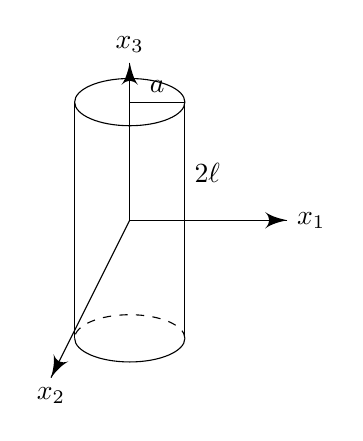
\begin{tikzpicture}
      \draw [->] (0, 0) -- (2, 0) node [right] {$x_1$};
      \draw [->] (0, 0) -- (0, 2) node [above] {$x_3$};
      \draw [->] (0, 0) -- (-1, -2) node [below] {$x_2$};
      \draw (0.7, -1.5) -- (0.7, 1.5) node [pos = 0.7, right] {$2\ell$};
      \draw (-0.7, -1.5) -- (-0.7, 1.5);
      \draw (0, 1.5) circle [x radius=0.7, y radius=0.3];
      \draw [dashed] (0.7, -1.5) arc (0:180:0.7 and 0.3);
      \draw (-0.7, -1.5) arc (180:360:0.7 and 0.3);
      \draw (0, 1.5) -- (0.7, 1.5) node [pos = 0.5, above] {$a$};
    \end{tikzpicture}
  \end{center}
  Use cylindrical polar coordinates:
  \begin{align*}
    x_1 &= r\cos \theta\\
    x_2 &= r\sin \theta\\
    x_3 &= x_3\\
    \d V &= r\;\d r\;\d \theta \;\d x_3
  \end{align*}
  We have
  \begin{align*}
    I_{33} &= \int_V \rho_0 (x_1^2 + x_2^2)\;\d V\\
    &= \rho_0 \int_0^a \int_0^{2\pi} \int_{-\ell}^\ell r^2 (r\;\d r\;\d \theta \;\d x_2)\\
    &= \rho_0 \cdot 2\pi \cdot 2\ell \left[\frac{r^4}{4}\right]_0^a\\
    &= \varepsilon_0 \pi \ell a^4.
  \end{align*}
  Similarly, we have
  \begin{align*}
    I_{11} &= \int_V \rho_0 (x_2^2 + x_3^2)\;\d V\\
    &= \rho_0 \int_0^a \int_0^{2\pi}\int_{-\ell}^\ell (r^2 \sin^2 \theta + x_3^2) r\;\d r\;\d \theta \;\d x_3\\
    &= \rho_0 \int_0^a \int_0^{2\pi} r\left(r^2 \sin^2 \theta\left[x_3\right]_{-\ell}^\ell + \left[\frac{x_3^3}{3}\right]^{\ell}_{-\ell}\right)\;\d \theta\;\d r\\
    &= \rho_0 \int_0^a \int_0^{2\pi} r\left(r^2 \sin^2 \theta 2\ell + \frac{2}{3}\ell^3\right)\;\d \theta\;\d r\\
    &= \rho_0 \left(2\pi a \cdot \frac{2}{3}\ell^3 + 2\ell\int_0^a r^2 \;\d r\int_0^{2\pi}\sin^2 \theta\right)\\
    &= \rho_0 \pi a^2 \ell\left(\frac{a^2}{2} + \frac{2}{3}\ell^2\right)
  \end{align*}
  By symmetry, the result for $I_{22}$ is the same.

  How about the off-diagonal elements?
  \begin{align*}
    I_{13} &= -\int_V \rho_0 x_1 x_3 \;\d V\\
    &= -\rho_0 \int_0^a \int_{-\ell}^\ell \int_0^{2\pi} r^2 \cos \theta x_3 \;\d r\;\d x_3 \;\d \theta\\
    &= 0
  \end{align*}
  Since $\int_0^{2\pi} \;\d \theta \cos \theta = 0$. Similarly, the other off-diagonal elements are all 0. So the non-zero components are
  \begin{align*}
    I_{33} &= \frac{1}{2}Ma^2\\
    I_{11} = I_{22} &= M\left(\frac{a^2}{4} + \frac{\ell^2}{3}\right)
  \end{align*}
  In the particular case where $\ell = \frac{a\sqrt{3}}{2}$, we have $I_{ij} = \frac{1}{2}ma^2 \delta_{ij}$. So in this case,
  \[
    \mathbf{L} = \frac{1}{2}Ma^2 \boldsymbol\omega
  \]
  for rotation about any axis.
\end{eg}

\subsection{Diagonalization of a symmetric second rank tensor}
Recall that using matrix notation,
\[
  T = (T_{ij}),\quad T' = (T_{ij}'),\quad R = (R_{ij}),
\]
and the tensor transformation rule $T'_{ij} = R_{ip}R_{jq}T_{pq}$ becomes
\[
  T' = RTR^T = RTR^{-1}.
\]
If $T$ is symmetric, it can be diagonalized by such an orthogonal transformation. This means that there exists a basis of orthonormal eigenvectors $\mathbf{e}_1, \mathbf{e}_2, \mathbf{e}_3$ for $T$ with real eigenvalues $\lambda_1, \lambda_2, \lambda_3$ respectively. The directions defined by $\mathbf{e}_1, \mathbf{e}_2, \mathbf{e}_3$ are the \emph{principal axes} for $T$, and the tensor is diagonal in Cartesian coordinates along these axes.

This applies to any symmetric rank-2 tensor. For the special case of the inertia tensor, the eigenvalues are called the \emph{principal moments of inertia}.

As exemplified in the previous example, we can often guess the correct principal axes for $I_{ij}$ based on the symmetries of the body. With the axes we chose, $I_{ij}$ was found to be diagonal by direct calculation.

\section{Invariant and isotropic tensors}
\subsection{Definitions and classification results}
\begin{defi}[Invariant and isotropic tensor]
  A tensor $T$ is \emph{invariant} under a particular rotation $R$ if
  \[
    T_{ij\cdots k}' = R_{ip}R_{jq}\cdots R_{kr}T_{pq\cdots r} = T_{ij\cdots k},
  \]
  ie. every component is unchanged under the rotation.

  A tensor $T$ which is invariant under every rotation is \emph{isotropic}, ie. the same in every direction.
\end{defi}

\begin{eg}
  The inertia tensor of a sphere is isotropic by symmetry.

  $\delta_{ij}$ and $\varepsilon_{ijk}$ are also isotropic tensors. This ensures that the component definitions of the scalar and vector products $\mathbf{a}\cdot \mathbf{b} = a_i b_j \delta_{ij}$ and $(\mathbf{a}\times \mathbf{b})_i = \varepsilon_{ijk} a_j b_k$ are independent of the Cartesian coordinate system.
\end{eg}

Isotropic tensors in $\R^3$ can be classified:
\begin{thm}\leavevmode
  \begin{enumerate}
    \item There are no isotropic tensors of rank 1, except the zero tensor.
    \item The most general rank 2 isotropic tensor is $T_{ij} = \alpha \delta_{ij}$ for some scalar $\alpha$.
    \item The most general rank 3 isotropic tensor is $T_{ijk} = \beta \varepsilon_{ijk}$ for some scalar $\beta$.
    \item All isotropic tensors of higher rank are obtained by combining $\delta_{ij}$ and $\varepsilon_{ijk}$ using tensor products, contractions, and linear combinations.
  \end{enumerate}
\end{thm}
We will provide a sketch of the proof:
\begin{proof}
  We analyze conditions for invariance under specific rotations through $\pi$ or $\pi/2$ about coordinate axes.

  \begin{enumerate}
    \item Suppose $T_i$ is rank-1 isotropic. Consider a rotation about $x_3$ through $\pi$:
      \[
        (R_{ij}) =
        \begin{pmatrix}
          -1 & 0 & 0\\
          0 & -1 & 0\\
          0 & 0 & 1
        \end{pmatrix}.
      \]
      We want $T_1 = R_{ip}T_p = R_{11} T_1 = -T_1$. So $T_1 = 0$. Similarly, $T_2 = 0$. By consider a rotation about, say $x_1$, we have $T_3 = 0$.
    \item Suppose $T_{ij}$ is rank-2 isotropic. Consider
      \[
        (R_{ij}) =
        \begin{pmatrix}
          0 & 1 & 0\\
          -1 & 0 & 0\\
          0 & 0 & 1
        \end{pmatrix},
      \]
      which is a rotation through $\pi/2$ about the $x_3$ axis. Then
      \[
        T_{13} = R_{1p}R_{3q} T_{pq} = R_{12}R_{33}T_{23} = T_{23}
      \]
      and
      \[
        T_{23} = R_{2p}R_{3q} T_{pq} = R_{21}R_{33}T_{13} = -T_{13}
      \]
      So $T_{13} = T_{23} = 0$. Similarly, we have $T_{31} = T_{32} = 0$.

      We also have
      \[
        T_{11} = R_{1p} R_{1q} T_{pq} = R_{12} R_{12}T_{22} = T_{22}.
      \]
      So $T_{11} = T_{22}$.

      By picking a rotation about a different axis, we have $T_{21} = T_{12}$ and $T_{22} = T_{33}$.

      Hence $T_{ij} = \alpha \delta_{ij}$.

    \item Suppose that $T_{ijk}$ is rank-3 isotropic. Using the rotation by $\pi$ about the $x_3$ axis, we have
      \[
        T_{133} = R_{1p}R_{3q}R_{3r}T_{pqr} = -T_{133}.
      \]
      So $T_{133} = 0$. We also have
      \[
        T_{111} = R_{1p}R_{1q}R_{1r}T_{pqr} = -T_{111}.
      \]
      So $T_{111} = 0$. We have similar results for $\pi$ rotations about other axes and other choices of indices.

      Then we can show that $T_{ijk} = 0$ unless all $i, j, k$ are distinct.

      Now consider
      \[
        (R_{ij}) =
        \begin{pmatrix}
          0 & 1 & 0\\
          -1 & 0 & 0\\
          0 & 0 & 1
        \end{pmatrix},
      \]
      a rotation about $x_3$ through $\pi/2$. Then
      \[
        T_{123} = R_{1p}R_{2q}R_{3r}T_{pqr} = R_{12}R_{21}R_{33}T_{213} -T_{213}.
      \]
      So $T_{123} = -T_{213}$. Along with similar results for other indices and axes of rotation, we find that $T_{ijk}$ is totally antisymmetric, and $T_{ijk} = \beta \varepsilon_{ijk}$ for some $\beta$.
  \end{enumerate}
\end{proof}
\begin{eg}
  The most general isotropic tensor of rank 4 is
  \[
    T_{ijk\ell} = \alpha \delta_{ij}\delta_{k\ell} + \beta \delta_{ik}\delta_{j\ell} + \gamma \delta_{i\ell}\delta_{jk}
  \]
  for some scalars $\alpha, \beta, \gamma$. There are no other independent combinations. (we might think we can write a rank-4 isotropic tensor in terms of $\varepsilon_{ijk}$, like $\varepsilon_{ijp}\varepsilon_{k\ell p}$, but this is just $\delta_{ik}\delta_{j\ell} - \delta_{i\ell}\delta_{jk}$. It turns out that anything you write with $\varepsilon_{ijk}$ can be written in terms of $\delta_{ij}$ instead)
\end{eg}

\subsection{Application to invariant integrals}
We have the following very useful theorem. It might seem a bit odd and arbitrary at first sight --- if so, read the example below first (after reading the statement of the theorem), and things will make sense!
\begin{thm}
  Let
  \[
    T_{ij\cdots k} = \int_V f(\mathbf{x}) x_i x_j \cdots x_k\;\d V.
  \]
  where $f(\mathbf{x})$ is a scalar function and $V$ is some volume.

  Given a rotation $R_{ij}$, consider an \emph{active} transformation: $\mathbf{x} = x_i \mathbf{e}_i$ is mapped to $\mathbf{x}' = x_i' \mathbf{e}_i$ with $x_i' = R_{ij} x_i$, ie. we map the components but not the basis, and $V$ is mapped to $V'$.

  Suppose that under this active transformation,
  \begin{enumerate}
    \item $f(\mathbf{x}) = f(\mathbf{x}')$,
    \item $V' = V$ (eg. if $V$ is all of space or a sphere).
  \end{enumerate}
  Then $T_{ij\cdots k}$ is invariant under the rotation.
\end{thm}

\begin{proof}
  First note that the Jacobian of the transformation $R$ is $1$, since it is simply the determinant of $R$ ($x_i' = R_{ip}x_p \Rightarrow \frac{\partial x_i'}{\partial x_p} = R_{ip}$), which is by definition 1. So $\d V = \d V'$.

  Then we have
  \begin{align*}
    R_{ip}R_{jq}\cdots R_{kr} T_{pq\cdots r} &= \int_V f(\mathbf{x})x_i' x_j' \cdots x_k' \;\d V\\
    &= \int_V f(\mathbf{x}')x_i' x_j' \cdots x_k'\;\d V&&\text{using (i)}\\
    &= \int_{V'} f(\mathbf{x}') x_i' x_j' \cdots x_k' \;\d V'&&\text{using (ii)}\\
    &= \int_{V} f(\mathbf{x}) x_i x_j \cdots x_k \;\d V&&\text{since $x_i$ and $x_i'$ are dummy}\\
    &= T_{ij\cdots k}
  \end{align*}
\end{proof}

The result is particularly useful if (1) and (2) hold for \emph{any} rotation $R$, in which case $T_{ij\cdots k}$ is isotropic.

\begin{eg}
  Let
  \[
    T_{ij} = \int_V x_i x_j \;\d V,
  \]
  with $V$ being a solid sphere of $|\mathbf{r}| < a$. Our result applies with $f = 1$, which, being a constant, is clearly invariant under rotations. Also the solid sphere is invariant under any rotation. So $T$ must be isotropic. But the only rank 2 isotropic tensor is $\alpha \delta_{ij}$. Hence we must have
  \[
    T_{ij} = \alpha \delta_{ij},
  \]
  and all we have to do is to determine the scalar $\alpha$.

  Taking the trace, we have
  \[
    T_{ii} = 3\alpha = \int_V x_i x_i \;\d V = 4\pi \int_0^a r^2 \cdot r^2\;\d r = \frac{4}{5}\pi a^5.
  \]
  So
  \[
    T_{ij} = \frac{4}{15}\pi a^5 \delta_{ij}.
  \]
  Normally if we are only interested in the $i \not= j$ case, we just claim that $T_{ij} = 0$ by saying ``by symmetry, it is $0$''. But now we can do it (more) rigorously!

  There is a closely related result for the inertia tensor of a solid sphere of constant density $\rho_0$, or of mass $M = \frac{4}{3}\pi a^3 \rho_0$.

  Recall that
  \[
    I_{ij} = \int_V \rho_0 (x_k x_k \delta_{ij} - x_i x_j)\;\d V.
  \]
  We see that $I_{ij}$ is isotropic (since we have just shown that $\int x_i x_j\;\d V$ is isotropic, and $x_kx_k \delta_{ij}$ is also isotropic). Let $I_{ij} = \beta \delta_{ij}$. Then
  \begin{align*}
    I_{ij} &= \int_V \rho_0 (x_k x_k \delta_{ij} - x_ix_j)\;\d V \\
    &= \rho_0\left(\delta_{ij}\int_V x_k x_k\;\d V - \int_V x_ix_j \;\d V\right)\\
    &= \rho_0\left(\delta_{ij}T_{kk} - T_{ij}\right)\\
    &= \rho_0\left(\frac{4}{5}\pi a^5\delta_{ij} - \frac{4}{15}\pi a^5 \delta_{ij}\right)\\
    &= \frac{8}{15}\rho_0 \pi a^5 \delta_{ij}\\
    &= \frac{2}{5}Ma^2 \delta_{ij}.
  \end{align*}
\end{eg}

\end{document}
